\RequirePackage[l2tabu, orthodox]{nag}
\documentclass[preprint,  11pt]{amsart}

\usepackage{mathrsfs}
\usepackage{fullpage}
\usepackage{natbib}
\usepackage[dvipsnames]{xcolor}

\linespread{1.28}

\usepackage{amsfonts}
\usepackage{amssymb}
\usepackage{amsmath}
\usepackage{amsthm}
\usepackage{amsbsy}
%\usepackage{natbib}
\usepackage{amssymb} % Without this \qed does not get filled square
\usepackage{verbatim}
\usepackage{bm} %for some types of bold letters
\usepackage{paralist} %Need to use \inparaenum
%\RequirePackage[dvips]{hyperref}
%\usepackage{lineno}
 \usepackage{color}
 \usepackage{mathrsfs}
 \usepackage{graphicx}
\usepackage{hyperref}
%\hypersetup{
%  colorlinks   = true, %Colours links instead of ugly boxes
%  urlcolor     = blue, %Colour for external hyperlinks
%  linkcolor    = blue, %Colour of internal links
%  citecolor   = red %Colour of citations
%}



% PROBABILITY RELATED
\newcommand{\E}{\mathbf{E}}
\def\P{\mathbf{P}}
\def\Filt{\mathcal F_{\bullet}} %filtration
\def\Var{\mbox{Var}}
\def\sd{\mbox{s.d.}}
\def\convd{\stackrel{d}{\rightarrow}}
\def\convp{\stackrel{P}{\rightarrow}}
\def\convas{\stackrel{a.s.}{\rightarrow}}
\def\convlp{\stackrel{L^{p}}{\rightarrow}}
\def\eqd{\stackrel{d}{=}}
\def\given{\left.\vphantom{\hbox{\Large (}}\right|}
%\def\Given{\left.\vphantom{\hbox{\large (}}\right|}
\def\Given{\ \pmb{\big|} \ }
\newcommand{\as}{$a.s.$}
\newcommand{\dist}{\mbox{\rm dist}}
\newcommand{\Poi}{\mbox{\rm Poi}}
\newcommand{\EE}[1]{\E\l[#1\r]}
\def\CN{CN}
\renewcommand\Re{\operatorname{Re}}
\renewcommand\Im{\operatorname{Im}}
%\renewcommand{\Pr}[1]{\,\mathbb P\,\(\,#1\,\)\,}
\newcommand\gauss{\ensuremath {e^{-x^{2}/2}}}
\DeclareMathOperator\erf{erf}
\newcommand\CRplus{\ensuremath{C[0,\infty)}}
\newcommand\CI{\ensuremath{C[0,1]}}


% COMMON MATHEMATICAL OBJECTS
\newcommand{\mat}[4]{\l[\begin{array}{cc}  #1 & #2 \\ #3 & #4  \end{array} \r]}
\newcommand{\vect}[2]{\l[\begin{array}{cc}  #1 \\ #2  \end{array} \r]}
\def\half{\frac{1}{2}}
\newcommand{\slfrac}[2]{\left.#1\middle/#2\right.}
\def\ccinf{C_c^{\infty}}
\newcommand{\one}{{\mathbf 1}}
\def\I#1{\mathbf{1}_{#1}}
\def\ind{{\mathbf 1}}
\newcommand\der[2]{\frac{d^{#1}}{d  #2^{#1}}}
%\renewcommand\matx[4]{\l[\begin{array}{cc}  #1 & #2 \\ #3 & #4\end{array} \r]}

% COMMON OPERATIONS
\def\summ{\sum\limits}
\def\intt{\int\limits}
\newcommand{\intg}[2]{\intt_{#1}^{#2}}
\def\doublint{\int\!\!\int}
\def\doublintfull{\intt_{-\infty}^{\infty}\!\!\intt_{-\infty}^{\infty}}
\def\prodd{\prod\limits}
\def\limm{\lim\limits}
\def\to{\rightarrow}
\def\tends{\rightarrow}
\def\fr{\frac}
\newcommand{\ontop}{\genfrac{}{}{0cm}{2}}
%\newcommand{\frac}[2]{\genfrac{}{}{}{}{#1}{#2}}
%\newcommand{\tfrac}[2]{\genfrac{}{}{}{1}{#1}{#2}}
%\newcommand{\binom}[2]{\genfrac{(}{)}{0pt}{}{#1}{#2}}
%\def\sgn{\mb{sgn}}
\def\d{\partial}
\def\dz{\frac{\partial }{ \partial z}}
\def\dzbar{\frac{\partial }{ \partial {\bar z}}}
\def\dw{\frac{\partial }{ \partial w}}
\def\dwbar{\frac{\partial }{ \partial {\bar zw}}}
\def\grad{\nabla}
\def\lap{\Delta}
\def\defn{\stackrel{\tiny def}{=}}
\def\di{\mbox{d}}
\newcommand{\diff}[1]{\frac{\partial}{\partial #1}}

% IMPORTANT MATH FUNCTIONS
\def\sgn{{\mb{sgn}}}
\newcommand\Tr{{\mbox{Tr}}}
\newcommand\tr{{\mbox{tr}}}
\def\per{\mb{per}}
\def\haf{\mb{haf}}
%\def\bar{\overline}
\newcommand{\Wi}[1]{:#1:}


% SPACINGS
\def\hsp{\hspace}
\def\mb{\mbox}
\newcommand{\head}[1]{{\noindent{\bfseries #1:}}}
\newcommand{\para}[1]{\vspace{6mm}\noindent{\bfseries #1:}}
\newcommand{\parau}[1]{\vspace{4mm}\noindent{\bfseries \underline{#1}:}}
\newcommand{\parag}[1]{\vspace{5mm}\noindent{\bfseries #1}}
\newcommand{\margin}[1]{\marginpar{\small \color{blue}{#1}}}

% BRACKETS AND BRACES
\def\Mid{\left\vert \right.}
\def\l{\left}
\def\r{\right}
\def\<{\langle}
\def\>{\rangle}

%\def\given{\left.\vphantom{\hbox{\Large (}}\right|}


% SHORTCUTS FOR ENVIRONMENTS
%\newcommand{\align}[1]{\begin{align*}#1\end{align*}}
\newcommand{\ba}{\[\begin{aligned}}
\newcommand{\ea}{\end{aligned}\]}
\newcommand\mnote[1]{} %off
\newcommand{\beq}[1]{\begin{equation}\label{#1}}
\newcommand\eeq{\end{equation}}
%\newcommand\be{\begin{align*}}
%\newcommand\ee{\end{align*}}
\newcommand\ben{\begin{equation}}
\newcommand\een{\end{equation}}
\newcommand\bes{\begin{eqnarray*}}
\newcommand\ees{\end{eqnarray*}}
\newcommand\besn{\begin{eqnarray}}
\newcommand\eesn{\end{eqnarray}}


\def\bthm{\begin{theorem}}
\def\ethm{\end{theorem}}
\def\bdefn{\begin{definition}}
\def\edefn{\end{definition}}
\newcommand{\benu}{\begin{enumerate}}
\newcommand{\beit}{\begin{itemize}}
\def\eenu{\end{enumerate}}
\def\eeit{\end{itemize}}
\def\beds{\begin{description}}
\def\eeds{\end{description}}
\def\bepr{\begin{problem}}
\def\eepr{\end{problem}}


\def\bprf{\begin{proof}}
\def\eprf{\end{proof}}
\def\berk{\begin{remark}}
\def\eerk{\end{remark}}
\def\bex{\begin{exercise}}
\def\eex{\end{exercise}}
\def\beg{\begin{example}}
\def\eeg{\end{example}}

% COMMON PHRASES
\newcommand\bllt{$\blacktriangleright$ \;\;}
\def\suchthat{{\; : \;}}
\renewcommand{\qed}{\hfill\text{$\blacksquare$}}
\newcommand*{\Cdot}{{\scalebox{2}{$\cdot$}}}

% CALLIGRAPHIC FONTS FOR GENERAL PURPOSE
\def\AA{{\mathcal A}}
\def\BB{{\mathcal B}}
\def \CC{{\mathcal C}}
\def\DD{{\mathcal D}}
\def\FF{{\mathcal F}}
\def\GG{{\mathcal G}}
\def\HH{{\mathcal H}}
\def\II{{\mathcal I}}
\def\JJ{{\mathcal J}}
\def \KK{{\mathcal K}}
\def\LL{{\mathbb L}}
\def\MM{{\mathcal M}}
\def\PP{{\mathcal P}}
\def\QQ{{\mathcal Q}}
\def\TT{{\mathcal T}}
\def\UU{{\mathcal U}}
\def\XX{{\mathcal X}}
\def\YY{{\mathcal Y}}
\def\ZZ{{\mathcal Z}}

% SETS OF REALS, INTEGERS, ETC.
\def\C{\mathbb{C}}
\def\D{\mathbb{D}} % unit disk
%\def\H{\mathbb H} % hyperbolic plane
%\renewcommand\H{{\varmathbb{H}}}
\def\N{\mathbb{N}}
\def\R{\mathbb{R}}
\def\Q{\mathbb{Q}}
\def\S{\mathbb{S}} % for sphere
\def\Z{\mathbb{Z}}
\def\Sym{{\mathcal S}} % symmetric group
\def\Uni{{\mathcal U}} % Unitary group


% SPECIALIZED SHORTCUTS
\newcommand{\intc}{\int_0^{2\pi}}
\newcommand{\supp}{\mbox{\textrm supp}}
\newcommand{\Arg}{\mbox{\textrm Arg}}
\newcommand{\Vol}{\mbox{\textrm Vol}}
\newcommand{\Cov}{\mbox{\textrm Cov}}
\newcommand{\sm}{{\raise0.3ex\hbox{$\scriptstyle \setminus$}}}
\newcommand{\agau}{a complex Gaussian analytic function}
\newcommand{\gi}{\,|\,}
\newcommand{\area}{\operatorname{area}}
\newcommand{\wA}{\widetilde{A}}
\newcommand{\zb}{\overline{z}}
\newcommand{\const}{\operatorname{const}}
\newcommand{\ip}[2]{\langle#1,#2\rangle}


% SPECIALIZED FONT USAGE
%\newcommand{\phi}{\varphi}


%  GREEK LETTERS
\def\alp{\alpha}
\def\bet{\beta}
\def\gam{\gamma}
\def\del{\delta}
\def\eps{\epsilon}
\renewcommand\phi{\varphi}
\def\kap{\kappa}
\def\lam{\lambda}
\def\ome{\omega}
\def\sig{{\sigma}}
\def\Sig{{\Sigma}}
\def\ups{\upsilon}
\def\zet{\zeta}
\def\Gam{\Gamma}
\def\Del{\Delta}
\def\Lam{\Lambda}
\def\Ome{\Omega}
%\newcommand\u{\mathbf{u}}
\renewcommand\u{\mathbf{u}}
\newcommand\x{\mathbf{x}}
\newcommand\y{\mathbf{y}}
\renewcommand\v{\mathbf{v}}
\newcommand\w{\mathbf{w}}




% THEOREM ENVIRONMENTS - DON'T REALLY UNDERSTAND ALL DETAILS BELOW
\theoremstyle{plain} %documentation says there are only three styles
                  %{plain},{definition},{remark}
%\theoremstyle{theorem}
    \newtheorem{theorem}{Theorem}
    \newtheorem{lemma}[theorem]{Lemma}
    \newtheorem{proposition}[theorem]{Proposition}
    \newtheorem{corollary}[theorem]{Corollary}
    \newtheorem{claim}[theorem]{Claim}
    \newtheorem{conjecture}[theorem]{Conjecture}


%    \newtheorem{proof}[proof]{Proof}

\theoremstyle{definition} % For roman text in the body
    \newtheorem{definition}[theorem]{Definition}
    \newtheorem{fact}[theorem]{Fact}
    \newtheorem{result}[theorem]{Result}
    \newtheorem{question}[theorem]{Question}
    \newtheorem{algorithm}[theorem]{Algorithm}
    \newtheorem{assumption}[theorem]{Assumption}
    \newtheorem{exercise}[theorem]{Exercise}
    \newtheorem{problem}[theorem]{Problem}
        \newtheorem{remark}[theorem]{Remark}
    \newtheorem{example}[theorem]{Example}

\newtheorem{protoeg}[theorem]{Example}
\newtheorem{protoremark}[theorem]{Remark}
\newtheorem{protodefinition}[theorem]{Definition}
\renewcommand{\theequation}{\arabic{equation}}
\renewcommand{\thetheorem}{\arabic{theorem}}


\def\newblock{\hskip .11em plus .33em minus .07em}


\def\t{{\bf t}}
\def\h{{\bf h}}
\def\omeg{\underline{\ome}}
\def\X{{\bf X}}
\def\Y{{\bf Y}}
%\newcommand{\para}[1]{\vspace{4mm}\noindent{\bf #1:}}
%\newcommand{\parag}[1]{\vspace{4mm}\noindent{\bf #1}}
\def\HH{\mathcal H}
\def\LL{\mathcal L}
\newcommand{\matrices}[4]{\l[\begin{array}{cc} #1 & #2 \\ #3 & #4  \end{array} \r]}
\def\doublintfull{\int\!\!\!\int}
\def\intg{\int\limits}
\def\half{\frac{1}{2}}
\def\sd{\mb{s.d.}}

\def\sig{{\sigma}}
\def\Sig{{\Sigma}}
\def\LL{{\mathbb L}}
\def\DD{{\mathcal D}}
\def\CC{{\mathcal C}}
\def\TT{{\mathcal T}}
\renewcommand\phi{{\varphi}}
\renewcommand{\benu}{\begin{enumerate}\setlength\itemsep{6pt}}
\renewcommand{\beit}{\begin{itemize}\setlength\itemsep{3pt}}
%\renewcommand\{Q}{\mathbf Q}

\renewcommand{\bex}{\indent\begin{exercise}}
\renewcommand\subset{\subseteq}
\def\mod{\left.\vphantom{\hbox{\Large (}}\right|}

\openup 0.4em

\usepackage{palatino}

\hypersetup{
    colorlinks=true, %set true if you want colored links
    linktoc=all,     %set to all if you want both sections and subsections linked
    linkcolor=blue,  %choose some color if you want links to stand out
}
\setcounter{tocdepth}{1}

\begin{document}

\title{Probability and Statistics}
\author{Manjunath Krishnapur}

\maketitle

 \tableofcontents

\newpage

\maketitle

\setcounter{page}{4}



\newpage
\vspace*{\fill}
\begin{center}
\Huge {\bf Probability}
\end{center}
\vspace*{\fill}
\newpage

\section{What is statistics and what is probability?}
Sometimes statistics is described as {\em the art or science of decision making in the face of uncertainty}.  Here are some examples to illustrate what it means.
\beg Recall the apocryphal story of two women who go to King Solomon with a child, each claiming that it is her own daughter. The solution according to the story uses human psychology and is not relevant to recall here. But is this a reasonable question that the king can decide?

Daughters resemble mothers to varying degrees, and one cannot be absolutely sure of guessing correctly.
 On the other hand, by comparing various features of the child with those of the two women, there is certainly a decent chance to guess correctly.

  If we could always get the right answer, or if we could never get it right, the question would not have been interesting. However, here we have uncertainty, but there is a decent chance of getting the right answer. That makes it interesting - for example, we can have a debate between {\em eyeists}  and {\em nosists} as to whether it is better to compare the eyes or the noses in arriving at a decision.
\eeg

\beg The IISc cricket team meets the Basavanagudi cricket club for a match. Unfortunately, the Basavanagudi team forgot to bring a coin to toss. The IISc captain helpfully offers his coin, but can he be trusted? What if he spent the previous night doctoring the coin so that it falls on one side with probability $3/4$ (or some other number)?

Instead of cricket, they could spend their time on the more interesting question of checking if the coin is {\em fair} or {\em biased}. Here is one way. If the coin is fair, in a large number of tosses, common sense suggests that we should get about equal number of heads and tails. So they  toss the coin 100 times. If the number of heads is exactly 50, perhaps they will agree that it is fair. If the number of heads is 90, perhaps they will agree that it is biased. What if the number of heads is 60? Or 35? Where and on what basis to draw the line between fair and biased? Again we are faced with the question of making decision in the face of uncertainty.
\eeg

\beg A psychic claims to have divine visions unavailable to most of us. You are assigned the task of testing her claims. You take a standard deck of cards, shuffle it well and keep it face down on the table. The psychic writes down the list of cards in some order - whatever her vision tells her about how the deck is ordered. Then you count the number of correct guesses. If the number is 1 or 2, perhaps you can dismiss her claims. If it is 45, perhaps you ought to be take her seriously. Again, where to draw the line?

The logic is this. Roughly one may say that {\em surprise} is just the name for our reaction to an event that we {\em \'{a} priori} thought to have low chance of occurring. Thus, we approach the experiment with the belief that the psychic is just guessing at random, and if the results are such that under that random-guess-hypothesis they have very small probability, then we are willing to be surprised, that is willing to discard our preconception and accept that she is a psychic.

How low a probability is surprising? In the context of psychics, let us say, $1/10000$. Once we fix that, we must find a number $m\le 52$ such that by pure guessing, the probability to get more than $m$ correct guesses is less that $1/10000$. Then we tell the psychic that if she gets more than $m$ correct guesses, we accept her claim, and otherwise, reject her claim.  This raises the simple (and you can do it yourself)
\begin{question} For a deck of $52$ cards, find the number $m$ such that
$$
\P(\mb{by random guessing we get more than }m\mb{ correct guesses})<\frac{1}{10000}.
$$
\end{question}
\eeg


\noindent{\bf{Summary:}} There are many situations in real life where one is required to make decisions under uncertainty. A general template for the answer could be to fix a small number that we allow as the probability of error, and deduce thresholds based on it. This brings us to the question of computing probabilities in various situations.



\vspace{4mm}
\noindent{\bf Probability:} Probability theory is a branch of pure mathematics, and forms the theoretical basis of statistics. In itself, probability theory has some basic objects and their relations (like real numbers, addition etc for analysis) and it makes no pretense of saying anything about the real world. Axioms are given and theorems are then deduced about these objects, just as in any other part of mathematics.

But a very important aspect of probability is that it is {\em applicable}. In other words, there are many real-world situations in which it is reasonable to take a model in probability and it turns out to reasonably replicate features of  the real-world situation.

In the example above, to compute the probability one must make the assumption that the deck of cards was completely shuffled. In other words, all possible 52! orders of the 52 cards are assumed to be equally likely. Whether this assumption is reasonable or not depends on how well the card was shuffled, whether the psychic was able to get a peek at the cards, whether some insider is informing the psychic of the cards etc. All these are non-mathematical questions, and must be decided on other basis.

\para{However...} Probability and statistics are very relevant in many situations that do not involve any uncertainty on the face of it. Here are some examples.
\beg {\em Compression of data}. Large files in a computer can be compressed to a .zip format and uncompressed when necessary. How is it possible to compress data like this? To give a very simple analogy, consider a long English word like {\em invertebrate}. If we take a novel and replace every occurrence of this word with ``zqz'', then  it is certainly possible to recover the original novel (since ``zqz'' does not occur anywhere else). But the reduction in size by replacing the 12-letter word by the 3-letter word is not much, since the word {\em invertebrate} does not occur often. Instead, if we replace the 4-letter word ``then'' by ``zqz'', then the total reduction obtained may be much higher, as the word ``then'' occurs quite often.

This suggests the following optimal way to represent words in English. The 26 most frequent words will be represented by single letters. The next $26\times 26$ most frequent words will be represented by two letter words, the next $26\times 26\times 26$ most frequent words by three-letter words, etc. Assuming there are no errors in transcription, this is a good way to reduce the size of any text document! Now, this involves knowing what the frequencies of occurrences of various words in actual texts are. Such statistics of usage of words are therefore clearly relevant (and they could be different for biology textbooks as compared to 19th century novels).
\eeg
\beg Search algorithms such as Google, use many randomized procedures. This cannot be explained right now, but let us give a simple reason to say why introducing randomness is a good idea in many situations. In the game of {\em rock-paper-scissors}, two people simultaneously shout one of the three words, rock, paper or scissors. The rule is that scissors beats paper, paper beats rock and rock beats scissors (if they both call the same word, they must repeat). In a game like this, although there is complete symmetry in the three items, it would be silly to have a fixed strategy. In other words, if you decide to always say rock, thinking that it doesn't matter which you choose, then your opponent can use that knowledge to always choose paper and thus win! In many games where the opponent gets to know your strategy (but not your move), the best strategy would involve  randomly choosing your move.
\eeg


%\newpage
\section{Discrete probability spaces}
\begin{definition} Let $\Omega$ be a finite or countable\footnote{For those unfamiliar with countable sets, it will be explained in some detail later.} set. Let $p:\Ome\to [0,1]$ be a function such that $\sum_{\ome\in \Ome}p_{\ome}=1$. Then $(\Ome,p)$ is called a {\em discrete probability space}. $\Ome$ is called the {\em sample space} and $p_{\ome}$ are called {\em elementary probabilities}.
\begin{itemize}
\item Any subset $A\subseteq \Ome$ is called an {\em event}. For an event $A$ we define its {\em probability} as $\P(A)=\sum_{\ome\in A}p_{\ome}$.
\item Any function $X:\Ome\to \R$ is called a {\em random variable}.  For a random variable we define its {\em expected value} or {\em mean} as $\E[X]=\sum_{\ome \in \Ome}X(\ome)p_{\ome}$.
\end{itemize}
\end{definition}

{\em\underline{ All of probability in one line}}: Take an (interesting) probability space $(\Ome, p)$ and an (interesting) event $A\subseteq \Ome$. Find $\P(A)$.



\vspace{2mm}
This is the mathematical side of the picture. It is easy to make up any number of probability spaces -  simply take a finite set and assign non-negative numbers to each element of the set so that the total is $1$.
\beg $\Ome=\{0,1\}$ and $p_{0}=p_{1}=\frac{1}{2}$. There are only four events here, $\emptyset, \{0\}, \{1\}$ and $\{0,1\}$. Their probabilities are, $0$, $1/2$, $1/2$ and $1$, respectively.
\eeg

\beg\label{eg:onecointoss} $\Ome=\{0,1\}$. Fix a number $0\le p \le 1$ and let $p_{1}=p$ and $p_{0}=1-p$. The sample space is the same as before, but the probability space is different for each value of $p$. Again there are only four events, and their probabilities are $\P\{\emptyset\}=0$, $\P\{0\}=1-p$, $\P\{1\}=p$ and $\P\{0,1\}=1$.
\eeg

\beg\label{eg:ncointosses} Fix a positive integer $n$. Let $$\Ome=\{0,1\}^{n}=\{\omeg\suchthat \omeg=(\ome_{1},\ldots ,\ome_{n})\mb{ with }\ome_{i}=0\mb{ or }1\mb{ for each }i\le n\}.$$
Let $p_{\omeg}=2^{-n}$ for each $\omeg\in \Ome$. Since $\Ome$ has $2^{n}$ elements, it follows that this is a valid assignment of elementary probabilities.

There are $2^{\#\Ome}=2^{2^{n}}$ events. One example is $A_{k}=\{\omeg\suchthat \omeg\in \Ome \mb{ and } \ome_{1}+\ldots +\ome_{n}=k
\}$ where $k$ is some fixed integer. In words, $A_{k}$ consists of those $n$-tuples of zeros and ones that have a total of $k$ many ones. Since there are $\binom{n}{k}$ ways to choose where to place these ones, we see that $\#A_{k}=\binom{n}{k}$. Consequently,
$$
\P\{A_{k}\}=\sum_{\omeg\in A_{k}}p_{\omeg} = \frac{\# A_{k}}{2^{n}}=\begin{cases} \binom{n}{k}2^{-n} &\mb{ if }0\le k\le n, \\ 0 & \mb{ otherwise}. \end{cases}
$$
It will be convenient to adopt the notation that $\binom{a}{b}=0$ if $a,b$ are positive integers and if $b>a$ or if $b<0$. Then we can simply write $\P\{A_{k}\}=\binom{n}{k}2^{-n}$ without having to split the values of $k$ into cases.
\eeg

\beg\label{eg:rballsinmbins} Fix two positive integers $r$ and $m$. Let
$$\Ome=\{\omeg\suchthat \omeg=(\ome_{1},\ldots ,\ome_{r}) \mb{ with }1\le \ome_{i} \le m \mb{ for each }i\le r\}.$$

The cardinality of $\Ome$ is $m^{r}$ (since each co-ordinate $\ome_{i}$ can take one of $m$ values). Hence, if we set $p_{\omeg}=m^{-r}$ for each $\omeg\in \Ome$, we get a valid probability space.

Of course, there are $2^{m^{r}}$ many events, which is quite large even for small numbers like $m=3$ and $r=4$. Some interesting events are $A=\{\omeg \suchthat \ome_{r}=1\}$, $B=\{\omeg\suchthat \ome_{i}\not=1 \mb{ for all }i\}$, $C=\{\omeg\suchthat \ome_{i}\not=\ome_{j} \mb{ if } i\not= j\}$. The reason why these are interesting will be explained later. Because of equal elementary probabilities, the probability of an event $S$ is just $\#S/m^{r}$.
\beit
\item Counting $A$: We have $m$ choices for each of  $\ome_{1},\ldots ,\ome_{r-1}$. There is only one choice for $\ome_{r}$. Hence $\#A=m^{r-1}$. Thus, $\P(A)=\frac{m^{r-1}}{m^{r}} = \frac{1}{m}$.
\item Counting $B$: We have $m-1$ choices for each $\ome_{i}$ (since $\ome_{i}$ cannot be $1$). Hence $\#B=(m-1)^{r}$ and thus $\P(B)=\frac{(m-1)^{r}}{m^{r}}=(1-\frac{1}{m})^{r}$.
\item Counting $C$: We must choose a distinct value for each $\ome_{1},\ldots ,\ome_{r}$. This is impossible if $m<r$. If $m\ge r$, then $\ome_{1}$ can be chosen as any of $m$ values. After $\ome_{1}$ is chosen, there are $(m-1)$ possible values for $\ome_{2}$, and then $(m-2)$ values for $\ome_{3}$ etc., all the way till $\ome_{r}$ which has $(m-r+1)$ choices. Thus, $\#C=m(m-1)\ldots (m-r+1)$. Note that we get the same answer if we choose $\ome_{i}$ in a different order (it would be strange if we did not!).

Thus, $\P(C)=\frac{m(m-1)\ldots (m-r+1)}{m^{r}}$. Note that this formula is also valid for $m<r$ since one of the factors on the right side is zero.
\eeit

\eeg


\subsection{Probability in the real world} In real life, there are often situations where there are several possible outcomes but which one will occur is unpredictable in some way. For example, when we toss a coin, we may get heads or tails. In such cases we use words such as {\em probability or chance}, {\em event or happening}, {\em randomness} etc.  What is the relationship between the intuitive and mathematical meanings of words such as probability or chance?

 In a given physical situation, we choose one out of all possible probability spaces that we think captures best the chance happenings in the situation. The chosen probability space is then called a {\em model} or a {\em probability model} for the given situation. Once the model has been chosen, calculation of probabilities of events therein is a mathematical problem. Whether the model really captures the given situation, or whether the model is inadequate and over-simplified is a non-mathematical question. Nevertheless that is an important question, and can be answered by observing the real life situation and comparing the outcomes with predictions made using the model\footnote{Roughly speaking we may divide the course into two parts according to these two issues. In the probability part of the course, we shall take many such models for granted and learn how to calculate or approximately calculate probabilities. In the statistics part of the course we shall see some methods by which we can arrive at such models, or test the validity of a proposed model.}.

 Now we describe several ``random experiments'' (a non-mathematical term to indicate a ``real-life'' phenomenon that is supposed to involve chance happenings) in which the previously given examples of probability spaces arise. Describing the probability space is the first step in any probability problem.

\begin{example} \para{Physical situation} Toss a coin. Randomness enters because we believe that the coin may turn up head or tail and that it is inherently unpredictable.

\para{The corresponding probability model} Since there are two outcomes, the sample space $\Ome=\{0,1\}$ (where we use $1$ for heads and $2$ for tails) is a clear choice. What about elementary probabilities? Under the equal chance hypothesis, we may take $p_{0}=p_{1}=\frac{1}{2}$. Then we have a probability model for the coin toss.

 If the coin was not fair, we would change the model by keeping $\Ome=\{0,1\}$ as before but letting $p_{1}=p$ and $p_{0}=1-p$ where the parameter  $p\in [0,1]$ is fixed.

Which model is correct? If the coin looks  symmetrical, then the two sides are equally likely to turn up, so the first model where $p_{1}=p_{0}=\half$ is reasonable. However, if the coin looks irregular, then theoretical considerations are usually inadequate to arrive at the value of $p$. Experimenting with the coin (by tossing it a large number of times) is the only way.

There is always an approximation in going from the real-world to a mathematical model. For example, the model above ignores the possibility that the coin can land on its side. If the coin is very thick, then it might be closer to a cylinder which can land in three ways and then we would have to modify the model...
\end{example}

Thus we see that example~\ref{eg:onecointoss} is a good model for a physical coin toss. What physical situations are captured by the probability spaces in example~\ref{eg:ncointosses} and example~\ref{eg:rballsinmbins}?

\para{Example~\ref{eg:ncointosses}} This probability space can be a model for tossing $n$ fair coins. It is clear in what sense, so we omit details for you to fill in.

The same probability space can also be a model for the tossing of the same coin $n$ times in succession. In this, we are implicitly assuming that the coin forgets the outcomes on the previous tosses. While that may seem obvious, it would be violated if our ``coin'' was a hollow lens filled with a semi-solid material like glue (then, depending on which way the coin fell on the first toss, the glue would settle more on the lower side and consequently the coin would be more likely to fall the same way again). This is a coin with memory!

\para{Example~\ref{eg:rballsinmbins}} There are several situations that can be captured by this probability space. We list some.
\beit
\item There are $r$ labelled balls and $m$ labelled bins. One by one, we put the balls into bins ``at random''. Then, by letting $\ome_{i}$ be the bin-number into which the $i^{\mb{\tiny th}}$ ball goes, we can capture the full configuration by the vector $\omeg=(\ome_{1},\ldots ,\ome_{n})$. If each ball is placed completely at random then the probabilities are $m^{-r}$ for each configuration $\omeg$.

In that example, $A$ is the event that the last ball ends up in the first bin, $B$ is the event that the first bin is empty and $C$ is the event that no bin contains more than one ball.
\item If $m=6$, then this may also be the model for throwing a fair die $r$ times. Then $\ome_{i}$ is the outcome on the $i^{\mb{\tiny th}}$ throw. Of course, it also models throwing $r$ different (and distinguishable) fair dice.
\item If $m=2$ and $r=n$, this is same as Example~\ref{eg:ncointosses}, and thus models the tossing of $n$ fair coins (or a fair coin $n$ times).
\item Let $m=365$. Omitting the possibility of leap years, this is a model for choosing $r$ people at random and noting their birthdays (which can be in any of $365$ ``bins''). If we assume that all days are equally likely as a birthday (is this really true?), then the same probability space is a model for this physical situation. In this example, $C$ is the event that no two people have the same birthday.
\eeit


The next example is more involved and interesting.
\beg \para{Real-life situation} Imagine a man-woman pair. Their first child is random, for example, the sex of the child, or the height to which the child will ultimately grow, etc cannot be predicted with certainty. How to make a probability model that captures the situation?

\para{A  possible probability model} Let there be $n$ genes in each human, and each of the genes can take two possible values (Mendel's ``factors''), which we denote as $0$ or $1$. Then, let $\Ome=\{0,1\}^{n}=\{\x=(x_{1},\ldots ,x_{n})\suchthat x_{i}=0 \mb{ or }1\}$. In this sense, each human being can be encoded as a vector in $\{0,1\}^{n}$.

To assign probabilities, one must know the parents. Let the two parents have gene sequences ${\bf a}=(a_{1},\ldots,a_{n})$ and ${\bf b}=(b_{1},\ldots ,b_{n})$. Then the possible offsprings gene sequences are in the set $\Ome_{0}:=\{\x\in \{0,1\}^{n}\suchthat x_{i}=a_{i} \mb{ or }b_{i}, \; \mb{ for each }i\le n\}$. Let $L:=\#\{i\suchthat a_{i}\not=b_{i}\}$.

One possible assignment of probabilities is that each of these offsprings is equally likely. In that case we can capture the situation in the following probability models.
\benu
\item Let $\Ome_{0}$ be the sample space and let $p_{\x}=2^{-L}$ for each $\x \in \Ome_{0}$.
\item Let $\Ome$ be the sample space and let $$p_{\x}=\begin{cases}2^{-L} & \mb{ if }\x\in \Ome_{0}\\ 0 & \mb{ if }\x \not\in \Ome_{0}. \end{cases}$$
\eenu
The second one has the advantage that if we change the parent pair, we don't have to change the sample space, only the elementary probabilities. What are some interesting events? Hypothetically, the susceptibility to a disease $X$ could be determined by the first ten genes, say the person is likely to get the disease if there are at-most four $1$s among the first ten. This would correspond to the event that $A=\{\x\in \Ome_{0}\suchthat x_{0}+\ldots+x_{10}\le 4\}$. (Caution: As far as I know, reading the genetic sequence to infer about the phenotype is still an impractical task in general).


\parag{Reasonable model?} There are many simplifications involved here. Firstly, genes are somewhat ill-defined concepts, better defined are nucleotides in the DNA (and even then there are two copies of each gene). Secondly, there are many ``errors'' in real DNA, even the total number of genes can change, there can be big chunks missing, a whole extra chromosome etc. Thirdly, the assumption that all possible gene-sequences in $\Ome_{0}$ are equally likely is incorrect - if two genes are physically close to each other in a chromosome, then they are likely to both come from the father or both from the mother. Lastly, if our interest originally was to guess the eventual height of the child or its intelligence, then it is not clear that these are determined by the genes alone (environmental factors such as availability of food etc. also matter). Finally, in case of the problem that Solomon faced, the information about genes of the parents was not available, the model as written would be use.
%Then, let $\Ome=to capture the situation is to take $\Ome=\{\mb{Black}, \mb{Brown}, \mb{Blue}, \mb{Green}\}$ (so we are assuming that these are all the possible colours). What about the assignment of elementary probabilities? The genes of the parents determine completely the possible combinations of genes that the child can get, and the chance of inheriting any particular combination of genes.
\eeg

\berk We have discussed at length the reasonability of the model in this example to indicate the enormous effort needed to find a sufficiently  accurate but also reasonably simple probability model for a real-world situation. Henceforth, we shall omit such caveats and simply switch back-and-forth between a real-world situation and a reasonable-looking probability model as if there is no difference between the two. However, thinking about the appropriateness of the chosen models is much encouraged.
\eerk

%\newpage
\section{Examples of discrete probability spaces}
\begin{example} \parag{Toss $n$ coins}. We saw this before, but assumed that the coins are fair. Now we do not.  The sample space is
$$
\Ome=\{0,1\}^{n}=\{\omeg=(\ome_{1},\ldots ,\ome_{n})\suchthat \ome_{i}=0 \mb{ or } 1 \mb{ for each }i\le n\}.
$$
Further we assign $p_{\omeg}=\alp_{\ome_{1}}^{(1)}\ldots \alp_{\ome_{n}}^{(n)}$. Here $\alp_{0}^{(j)}$ and $\alp_{1}^{(j)}$ are supposed to indicate the probabilities that the $j^{\mb{th}}$ coin falls tails up or heads up, respectively. Why did we take the product of $\alp^{(j)}_{\cdot}$s and not some other combination? This is a non-mathematical question about what model is suited for the given real-life example. For now, the only justification is that empirically the above model seems to capture the real life situation accurately.

In particular, if the $n$ coins are identical, we may write $p=\alp_{1}^{(j)}$ (for any $j$) and the elementary probabilities become  $p_{\omeg}=p^{\sum_{i}\ome_{i}}q^{n-\sum_{i}\ome_{i}}$ where $q=1-p$.

Fix $0\le k\le n$ and let $B_{k}=\{\omeg\suchthat \sum_{i=1}^{n}\ome_{i}=k\}$ be the event that we see exactly $k$ heads out of $n$ tosses. Then $\P(B_{k})=\binom{n}{k}p^{k}q^{n-k}$. If $A_{k}$ is the event that there are at least $k$ heads, then
$\P(A_{k})=\summ_{\ell=k}^{n}\binom{n}{\ell}p^{\ell}q^{n-\ell}$.
\end{example}

\begin{example} \parag{Toss a coin $n$ times}. Again
\begin{align*}
\Ome=\{0,1\}^{n}&=\{\omeg=(\ome_{1},\ldots ,\ome_{n})\suchthat \ome_{i}=0 \mb{ or } 1 \mb{ for each }i\le n\}, \\
p_{\omeg}&=p^{\sum_{i}\ome_{i}}q^{n-\sum_{i}\ome_{i}}.
\end{align*}
This is the same probability space that we got for the tossing of $n$ identical looking coins. Implicit is the assumption that once a coin is tossed, for the next toss it is as good as a different coin but with the same $p$. It is possible to imagine a world where coins retain the memory of what happened before (or as explained before, we can make a ``coin'' that remembers previous tosses!), in which case this would not be a good model for the given situation. We don't believe that this is the case for coins in our world, and this can be verified empirically.
\end{example}

\begin{example} \parag{Shuffle a deck of 52 cards}. $\Ome=S_{52}$, the set of all permutations\footnote{We use the notation $[n]$ to denote the set $\{1,2,\ldots ,n\}$. A permutation of $[n]$ is a vector $(i_{1},i_{2},\ldots ,i_{n})$ where $i_{1},\ldots ,i_{n}$ are distinct elements of $[n]$, in other words, they are $1,2,\ldots ,n$ but in some order. Mathematically, we may define a permutation as a bijection $\pi:[n]\to [n]$. Indeed, for a bijection $\pi$, the numbers $\pi(1),\ldots ,\pi(n)$ are just $1,2,\ldots ,n$ in some order.} of $[52]$ and $p_{\pi}=\frac{1}{52!}$ for each $\pi\in S_{52}$. More generally, we can make a model for a deck of $n$ cards, in which case the sample space is $S_n$ and elementary probabilities are $1/n!$ for each $n$.

As an illustration, when $n=3$, the sample space is
\begin{align*}
S_3=\l\{(1,2,3), (1,3,2), (2,3,1), (2,1,3), (3,1,2), (3,2,1) \r\}
\end{align*}
where $(2,3,1)$ denotes the deck where the top card is $2$, the next one is $3$ and the bottom card is $1$. The elementary probabilities are all $1/6$ in this case.
\end{example}

\beg \parag{``Psychic'' guesses a deck of cards}. The sample space is $\Ome=S_{52}\times S_{52}$ and $p_{(\pi,\sig)}=1/(52!)^{2}$ for each pair $(\pi,\sig)$ of permutations. In a pair $(\pi,\sig)$, the permutation $\pi$ denotes the actual order of  cards in the shuffled deck, and $\sig$ denotes the order guessed by the psychic. If the guesses are purely random, then the probabilities are as we have written.

An interesting random variable is the number of correct guesses. This is the function $X:\Ome\to \R$ defined by $X(\pi,\sig)=\sum_{i=1}^{52}\one_{\pi_{i}=\sig_{i}}$. Correspondingly we have the events $A_{k}=\{(\pi,\sig)\suchthat X(\pi,\sig)\ge k\}$.
\eeg

\begin{example} \parag{Toss a coin till a head turns up}. $\Ome=\{1,01,001,0001,\ldots \}\cup\{\bar{0}\}$. Let us write $0^{k}1=0\ldots01$ as a short form for $k$ zeros (tails) followed by $1$ and $\bar{0}$ stands for the sequence of all tails. Let $p\in [0,1]$. Then, we set $p_{0^{k}1}=q^{k}p$ for each $k\in \N$. We also set $p_{\bar{0}}=0$ if $p>0$ and $p_{\bar{0}}=1$ if $p=0$. This is forced on us by the requirement that elementary probabilities add to $1$.

Let $A=\{0^{k}1\suchthat k\ge n\}$ be the event that at least $n$ tails fall before a head turns up. Then $\P(A)=q^{n}p+q^{n+1}p+\ldots =q^{n}$.
\end{example}

\begin{example} \parag{Place $r$ distinguishable balls in $m$ distinguishable urns at random}. We saw this before (the words ``labelled'' and ``distinguishable'' mean the same thing here). The sample space is $\Ome=[m]^{r}=\{\omeg=(\ome_{1},\ldots ,\ome_{r})\suchthat 1\le \ome_{i}\le m\}$ and $p_{\omeg}=m^{-r}$ for every $\omeg\in \Ome$. Here $\ome_{i}$ indicates the urn number into which the $i^{\mb{th}}$ ball goes.
\end{example}

\beg \parag{Birthday ``paradox''} There are $n$ people at a party. What is the chance that two of them have the same birthday?

This can be thought of as a balls in bin problem, where the bins are labelled $1,2,\ldots ,365$ (days of the year), and the balls are labelled $1,2,\ldots ,n$ (people). The sample space can be copied from the previous example with $r=n$ and $m=365$. In doing this, we have omitted the possibility of February 29th, which simplifies our life a little bit. What are the elementary probabilities? Let us assume that all sample points have equal probability\footnote{This assumption is not entirely realistic, for example, Figure~\ref{fig:birthdaysUS1969to1988} shows actual data from a specific geographic location over a specific period of time. Seasonal variation is apparent! In addition there are complications such as the possibility of a pair of twins attending the party.}.
\eeg
\begin{figure}\label{fig:birthdaysUS1969to1988}
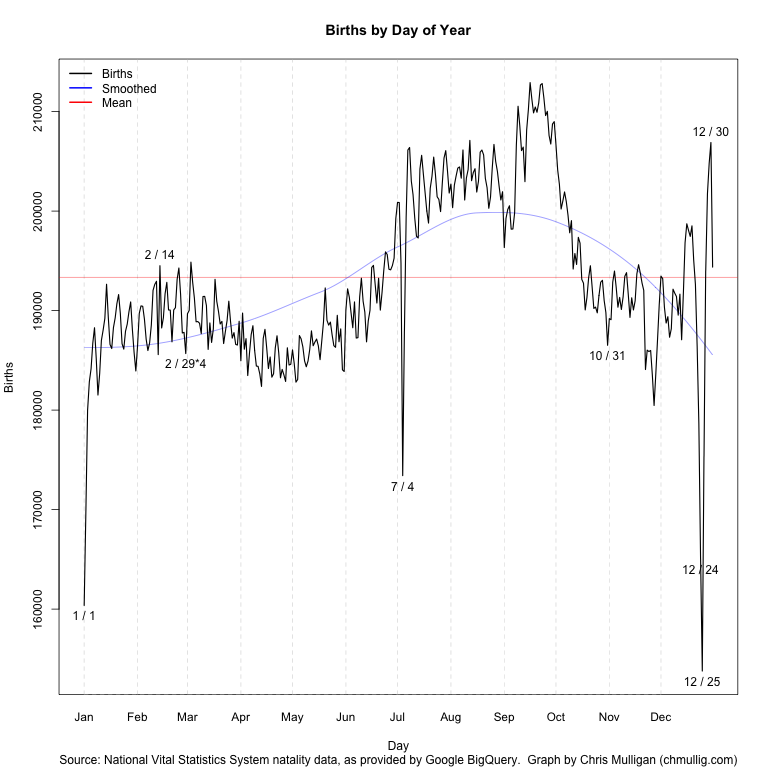
\includegraphics[scale=0.3]{birthdaysUS1969to1988}
%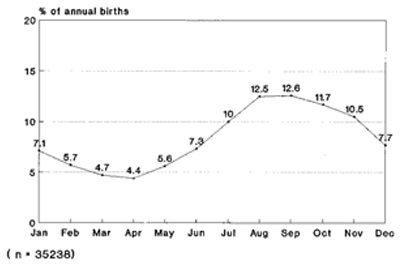
\includegraphics[scale=0.3]{birthdaysHaryana1972to1990}
\caption{Frequencies of birthdays in the United States of America from 1969 to 1988. Data taken from \href{http://andrewgelman.com/2012/06/12/simple-graph-win-the-example-of-birthday-frequencies/}{Andrew Gelman}.}
\end{figure}
The event of interest is that there is at least one bin that has at least two balls. In other words,
\ba
A=\{\omeg=(\ome_1,\ldots ,\ome_n)\suchthat \ome_i=\ome_j \mb{ for some }i<j\}.
\ea
In this case, it is easier to calculate the probability of
\ba
A^c=\{\omeg=(\ome_1,\ldots ,\ome_n)\suchthat \ome_i\not=\ome_j \mb{ for all }i<j\}.
\ea
Indeed, the cardinality of $A^c$ is $m(m-1)\ldots (n-m+1)$ (each person has to be assigned a different birthday), whence
\ba
\P(A)=1-\frac{m(m-1)\ldots (m-n+1)}{m^r}.
\ea
If $n>m$, the probability is obviously zero. The reason this is called a ``paradox'' is that even for $n$ much smaller than $m$, the probability becomes significantly large. For example, for $m=365$, here are the probabilities for a few values of $n$:
\begin{align*}
\begin{array}{c||c|c|c|c|c}
n & 5 & 15 & 25 & 35 & 45 \\ \hline
\P(A) & 0.027 & 0.253 &  0.569 &  0.814 & 0.941
\end{array}
\end{align*}

\begin{example} \parag{Place $r$ indistinguishable balls in $m$ distinguishable urns at random}.
Since the balls are indistinguishable, we can only count the number of balls in each urn. The sample space is
$$
 \Ome=\{(\ell_{1},\ldots ,\ell_{m})\suchthat \ell_{i}\ge 0, \; \ell_{1}+\ldots +\ell_{m}=r\}.
$$
We give two proposals for the elementary probabilities.
\benu
\item Let $p^{\mb{\tiny MB}}_{(\ell_{1},\ldots ,\ell_{m})}=\frac{m!}{\ell_{1}!\ell_{2}!\ldots \ell_{m}!}\frac{1}{m^{r}}$. These are the probabilities that result if we place $r$ labelled balls in $m$ labelled urns, and then erase the labels on the balls.
%Let $\Ome_{\mb{\tiny MB}}=\{(1,1),(1,2),(2,1),(2,2)\}$ and $p_{\ome}=1/4$ for each $\ome\in \Ome_{\mb{\tiny MB}}$. Here $(1,1)$ indicates that the first ball is in the first urn and the second ball also is in the first urn etc. If the balls are labelled, then $\Ome_{\mb{\tiny MB}}$ is the space of all distinguishable configurations. Elementary probabilities are chosen so that all distinguishable configurations are equally likely.
\item Let $p^{\mb{\tiny BE}}_{(\ell_{1},\ldots ,\ell_{m})}=\frac{1}{\binom{m+r-1}{r-1}}$ for each $(\ell_{1},\ldots ,\ell_{m})\in \Ome$. Elementary probabilities are chosen so that all distinguishable configurations are equally likely.
\eenu
That these are legitimate probability spaces depend on two combinatorial facts.
\bex
\benu
\item Let $(\ell_{1},\ldots ,\ell_{m})\in \Ome$. Show that $\#\{\omeg\in [m]^{r} \suchthat \sum_{j=1}^{r}\one_{\ome_{j}=i}=\ell_{i} \mb{ for each }i\in [m]\} = \frac{n!}{\ell_{1}!\ell_{2}!\ldots \ell_{m}!}$. Hence or directly, show that $\summ_{\ome\in \Ome}p_{\ome}^{\tiny MB}=1$.
\item Show that $\# \Ome = \binom{m+r-1}{r-1}$. Hence, $\summ_{\ome\in \Ome}p_{\ome}^{\tiny BE}=1$.
\eenu

\eex

The two models are clearly different. Which one captures reality? We can arbitrarily label the balls for our convenience, and then erase the labels in the end. This clearly yields elementary probabilities $p^{\tiny MB}$. Or to put it another way, pick the balls one by one and assign them randomly to one of the urns. This suggests that $p^{\tiny MB}$ is the ``right one''.

This leaves open the question of whether there is a natural mechanism of assigning balls to urns so that the probabilities $p^{\tiny BE}$ shows up. No such mechanism has been found. But this probability space does occur in the physical world. If $r$ photons (``indistinguishable balls'') are to occupy $m$ energy levels (``urns''), then empirically it has been verified that the correct probability space is the second one!\footnote{The probabilities $p^{\mb{\tiny MB}}$ and $p^{\mb{\tiny BE}}$ are called Maxwell-Boltzmann statistics and Bose-Einstein statistics. There is a third kind, called Fermi-Dirac statistics which is obeyed by electrons. For general $m\ge r$,  the sample space is $\Ome_{\mb{\tiny FD}}=\{(\ell_{1},\ldots ,\ell_{m})\suchthat \ell_{i}=0 \mb{ or }1 \mb{ and }\ell_{1}+\ldots +\ell_{m}=r\}$ with equal probabilities for each element. In words, all distinguishable configurations are equally likely, with the added constraint that at most one electron can occupy each energy level.}
\end{example}




\beg \parag{Sampling with replacement from a population}. Define $\Ome=\{\omeg\in [N]^{k}\suchthat \ome_{i}\in [N] \mb{ for }1\le i\le k\}$ with $p_{\omeg}=1/N^{k}$ for each $\omeg\in \Ome$. Here $[N]$ is the population (so the size of the population is $N$) and the size of the sample is $k$. Often the language used is of a box with $N$ coupons from which $k$ are drawn with replacement.
\eeg

\beg \parag{Sampling without replacement from a population}. Now we take
\begin{align*}
\Ome=\l\{\omeg\in [N]^{k}\suchthat \ome_{i}\mb{ are distinct elements of } [N]\r\}, \\
p_{\omeg}=\frac{1}{N(N-1)\ldots (N-k+1)}  \mb{ for each }\omeg\in \Ome.
\end{align*}

Fix $m<N$ and define the random variable $X(\omeg)=\sum_{i=1}^{k}\one_{\ome_{i}\le m}$. If the population $[N]$ contains a subset, say $[m]$, (could be the subset of people having a certain disease), then $X(\omeg)$ counts the number of people in the sample who have the disease. Using $X$ one can define  events such as $A=\{\omeg\suchthat X(\omeg)=\ell\}$ for some $\ell\le m$. If $\omeg\in A$, then $\ell$ of the $\ome_{i}$ must be in $[m]$ and the rest in $[N]\setminus [m]$. Hence $$\#A=\binom{k}{\ell}m(m-1)\ldots (m-\ell+1)(N-m)(N-m-1)\ldots (N-m-(k-\ell)+1).$$
As the probabilities are equal for all sample points, we get
\begin{align*}
\P(A)&= \frac{\binom{k}{\ell}m(m-1)\ldots (m-\ell+1)(N-m)(N-m-1)\ldots (N-m-(k-\ell)+1)}{N(N-1)\ldots (N-k+1)} \\
 &= \frac{1}{\binom{N}{k}}\binom{m}{\ell}\binom{N-m}{k-\ell}.
\end{align*}
This expression arises whenever the population is subdivided into two parts and we count the number of samples that fall in one of the sub-populations.
\eeg

\begin{example}\parag{Gibbs measures}. Let $\Ome$ be a finite set and let $\HH:\Ome\to \R$ be a function. Fix $\beta\ge 0$. Define $Z_{\beta}=\sum_{\ome}e^{-\beta \HH(\ome)}$ and then set $p_{\ome}=\frac{1}{Z_{\beta}}e^{-\beta \HH(\ome)}$. This is clearly a valid assignment of probabilities.

This is a class of examples from statistical physics. In that context, $\Ome$ is the set of all possible states of a system and $\HH(\ome)$ is the energy of the state $\ome$. In mechanics a system settles down to the state with the lowest possible energy, but if there are thermal fluctuations (meaning the ambient temperature is not absolute zero), then the system may also be found in other states, but higher energies are less and less likely. In the above assignment, for two states $\ome$ and $\ome'$, we see that $p_{\ome}/p_{\ome'}=e^{\beta (\HH(\ome')-\HH(\ome))}$ showing that higher energy states are less probable. When $\beta=0$, we get $p_{\ome}=1/|\Ome|$, the uniform distribution on $\Ome$. In statistical physics, $\beta$ is equated to $1/\kap T$ where $T$ is the temperature and $\kappa$ is Boltzmann's constant.

Different physical systems are defined by choosing $\Ome$ and $\HH$ differently. Hence this provides a rich class of examples which are of great importance in probability.
\end{example}

It may seem that probability is trivial, since the only problem is to find the sum of $p_{\ome}$ for $\ome$ belonging to event of interest. This is far from the case. The following example is an illustration.

\begin{example}\parag{Percolation}. Fix $m,n$ and consider a rectangle in $\Z^{2}$, $R=\{(i,j)\in \Z^{2}\suchthat 0\le i\le n, \ 0\le j\le m\}$. Draw this on the plane along with the grid lines. We see $(m+1)n$ horizontal edges and $(n+1)m$ vertical edges. Let $E$ be the set of $N=(m+1)n+(n+1)m$ edges and let $\Ome$ be the set of all subsets of $E$. Then $|\Ome|=2^{N}$. Let $p_{\ome}=2^{-N}$ for each $\ome \in \Ome$. An interesting event is
\begin{align*}
A=\{\ome \in \Ome\suchthat & \mb{ the subset of edges in }\ome \\
 & \mb{ connect  the top side of }R \mb{ to the bottom side of }R\}.
\end{align*}

This may be thought of as follows. Imagine that each edge is a pipe through which water can flow. However each tube may be blocked or open. $\ome$ is the subset of pipes that are open. Now pour water at the top of the rectangle $R$. Will water trickle down to the bottom? The answer is yes if and only if $\ome$ belongs to $A$.

Finding $\P(A)$ is a very difficult problem. When $n$ is large and $m=2 n$, it is expected that $\P(A)$ converges to a specific number, but proving it is an open problem as of today!\footnote{In a very similar problem on a triangular lattice, it was proved by Stanislav Smirnov (2001) for which he won a fields medal. Proof that computing probabilities is not always trivial!}
\end{example}



We now give two non-examples.
\begin{example}\parag{A non-example - Pick a natural number uniformly at random}. The sample space is clearly $\Ome=\N=\{1,2,3,\ldots\}$. The phrase ``uniformly at random'' suggests that the elementary probabilities should be the same for all elements. That is $p_{i}=p$ for all $i\in \N$ for some $p$. If $p=0$, then $\sum_{i\in \N}p_{i}=0$ whereas if $p>0$, then $\sum_{i\in \N}p_{i}=\infty$. This means that there is no way to assign elementary probabilities so that each number has the same chance to be picked.

This appears obvious, but many folklore puzzles and paradoxes in probability are based on the faulty assumption that it is possible to pick a natural number at random. For example, when asked a question like ``What is the probability that a random integer is odd?'', many people answer $1/2$. We want to emphasize that the probability space has to be defined first, and only then can probabilities of events be calculated. Thus, the question does not make sense to us and we do not have to answer it!\footnote{For those interested, there is one way to make sense of such questions. It is to consider a sequence of probability spaces $\Ome^{(n)}=\{1,2,\ldots ,n\}$ with elementary probabilities $p^{(n)}_{i}=1/n$ for each $i\in \Ome_{n}$. Then, for a subset $A\subseteq \Z$, we consider $\P_{n}(A\cap \Ome_{n})=\#(A\cap [n])/n$. If these probabilities converge to a limit $x$ as $n\to \infty$, then we could say that $A$ has asymptotic probability $x$. In this sense, the set of odd numbers does have  asymptotic probability $1/2$, the set of numbers divisible by $7$ has asymptotic probability $1/7$ and the set of prime numbers has asymptotic probability $0$. However, this notion of asymptotic probability has many shortcomings. Many subsets of natural numbers will not have an asymptotic probability, and even sets which do have asymptotic probability fail to satisfy basic rules of probability that we shall see later. Hence, we shall keep such examples out of our system.}
\end{example}

\begin{example}\parag{Another non-example - Throwing darts}. A dart is thrown at a circular dart board. We assume that the dart does hit the board but were it hits is ``random'' in the same sense in which we say the a coin toss is random. Intuitively this appears to make sense. However our framework is not general enough to incorporate this example. Let us see why.

The dart board can be considered to be the disk $\Ome=\{(x,y)\suchthat x^{2}+y^{2}\le r^{2}\}$ of given radius $r$. This is an uncountable set. We cannot assign elementary probabilities $p_{(x,y)}$ for each $(x,y)\in \Ome$ in any reasonable way. In fact the only reasonable assignment would be to set $p_{(x,y)}=0$ for each $(x,y)$ but then what is $\P(A)$ for a subset $A$? Uncountable sums are not well defined.

We need a branch of mathematics called {\em measure theory} to make proper sense of uncountable probability spaces. This will not be done in this course although we shall later say a bit about the difficulties involved. The same difficulty shows up in the following ``random experiments'' also.
\benu
\item \parag{Draw a number at random from the interval $[0,1]$}. $\Ome=[0,1]$ which is uncountable.
\item \parag{Toss a fair coin infinitely many times}. $\Ome=\{0,1\}^{\N}:=\{\omeg=(\ome_{1},\ome_{2},\ldots )\suchthat \ome_{i}=0 \mb{ or }1\}$. This is again an uncountable set.
\eenu
\end{example}
\berk In one sense, the first non-example is almost irredeemable but  the second non-example can be dealt with, except for technicalities beyond this course. We shall later give a set of working rules to work with such ``continuous probabilities''. Fully satisfactory development will have to wait for a course in measure theory.
\eerk




\section{Basic rules of probability}
So far we have defined the notion of probability space and probability of an event. But most often, we do not calculate probabilities from the definition. This is like in integration, where one defined the integral of a function as a limit of Riemann sums, but that definition is used only to find integrals of $x^{n}$, $\sin(x)$ and a few such functions. Instead, integrals of complicated expressions such as $x\sin(x)+2\cos^{2}(x)\tan(x)$ are calculated by various rules, such as substitution rule, integration by parts etc. In probability we need some similar rules relating probabilities of various combinations of events to the individual probabilities.


\begin{proposition}\label{prop:basicrules} Let $(\Ome,p_{\cdot})$ be a discrete probability space.
\benu
\item For any event $A$, we have $0\le \P(A)\le 1$. Also, $\P(\emptyset)=0$ and $\P(\Ome)=1$.
\item {\em Finite additivity of probability:} If $A_{1},\ldots ,A_{n}$ are pairwise disjoint events, then $\P(A_{1}\cup \ldots \cup A_{n})=\P(A_{1})+\ldots +\P(A_{n})$.
In particular, $\P(A^{c})=1-\P(A)$ for any event $A$.
\item {\em Countable additivity of probability:} If $A_{1},A_{2},\ldots$ is a countable collection of pairwise disjoint events, then $\P(\cup A_{i})=\sum_{i}\P(A_{i})$.
\eenu
\end{proposition}
All of these may seem obvious, and indeed they would be totally obvious if we stuck to finite sample spaces. But the sample space could be countable, and then probability of events may involve infinite sums which need special care in manipulation. Therefore we must give a proof. In writing a proof, and in many future contexts, it is useful to introduce the following notation.

\para{Notation} Let $A\subseteq \Ome$ be an event. Then, we define a function $\one_{A}:\Ome\to \R$, called the {\em indicator function of $A$},  as follows.
$$
\one_{A}(\ome) = \begin{cases}
1 & \mb{ if }\ome\in A,\\
0 & \mb{ if }\ome\not\in A.
\end{cases}
$$
Since a function from $\Ome$ to $\R$ is called a random variable, the indicator of any event is a random variable. All information about the event $A$ is in its indicator function (meaning, if we know the value of $\one_{A}(\ome)$, we know whether or not $\ome$ belongs to $A$). For example, we can write $\P(A)=\sum_{\ome\in \Ome}\one_{A}(\ome)p_{\ome}$.

Now we prove the proposition.
\bprf
\benu
\item By definition of probability space $\P(\Ome)=1$ and $\P(\emptyset)=0$. If $A$ is any event, then $\one_{\emptyset}(\ome)p_{\ome}\le \one_{A}(\ome)p_{\ome}\le \one_{\Ome}(\ome)p_{\ome}$. By Exercise~\ref{ex:linearitymonotonicityofsums}, we get
$$
\sum_{\ome\in \Ome}\one_{\emptyset}(\ome)p_{\ome} \le \sum_{\ome\in \Ome}\one_{A}(\ome)p_{\ome} \le \sum_{\ome\in \Ome}\one_{\Ome}(\ome)p_{\ome}.
$$
As observed earlier, these sums are just $\P(\emptyset)$, $\P(A)$ and $\P(\Ome)$, respectively. Thus, $0\le \P(A)\le 1$.
\item It suffices to prove it for two sets (why?). Let $A,B$ be two events such that $A\cap B=\emptyset$. Let $f(\ome)=p_{\ome}\one_{A}(\ome)$ and $g(\ome)=p_{\ome}\one_{B}(\ome)$ and $h(\ome)=p_{\ome}\one_{A\cup B}(\ome)$. Then, the disjointness of $A$ and $B$ implies that $f(\ome)+g(\ome)=h(\ome)$ for all $\ome\in \Ome$. Thus, by Exercise~\ref{ex:linearitymonotonicityofsums}, we get
$$
\sum_{\ome\in \Ome}f(\ome)+\sum_{\ome\in \Ome}g(\ome) = \sum_{\ome\in \Ome}h(\ome).
$$
But the three sums here are precisely $\P(A)$, $\P(B)$ and $\P(A\cup B)$. Thus, we get $\P(A\cup B)=\P(A)+\P(B)$.
\item This is similar to finite additivity but needs a more involved argument. We leave it as an exercise for the interested reader. \qedhere
\eenu
\eprf
\bex Adapt the proof to prove that for a countable family of events $A_{k}$ in a common probability space (no disjointness assumed), we have
$$
\P(\cup_{k}A_{k})\le \sum_{k}\P(A_{k}).
$$
\eex

\bdefn[Limsup and liminf of sets] If $A_{k}$, $k\ge 1$, is a sequence of subsets of $\Ome$, we define
\begin{equation*}
\limsup A_{k}=\bigcap_{N=1}^{\infty}\bigcup_{k=N}^{\infty}A_{k}, \qquad \mb{ and } \qquad  \liminf A_{k}=\bigcup_{N=1}^{\infty}\bigcap_{k=N}^{\infty}A_{k}.
\end{equation*}
In words, $\limsup A_{k}$ is the set of all $\ome$ that belong to infinitely many of the $A_{k}$s, and $\liminf A_{k}$ is the set of all $\ome$ that belong to all but finitely many of the $A_{k}$s.

Two special cases are of increasing and decreasing sequences of events. This means $A_{1}\subseteq A_{2}\subseteq A_{3}\subseteq \ldots$ and $A_{1}\supseteq A_{2}\supseteq A_{3}\supseteq \ldots$. In these cases, the limsup and liminf are the same (so we refer to it as the limit of the sequence of sets). It is $\cup_{k}A_{k}$ in the case of increasing events and $\cap_{k}A_{k}$ in the case of decreasing events.
\edefn

\bex Events below are all contained in a discrete probability space. Use countable additivity of probability to show that
\benu
\item If $A_{k}$ are increasing events with limit $A$, show that $\P(A)$ is the increasing limit of $\P(A_{k})$.
\item If $A_{k}$ are decreasing events with limit $A$, show that $\P(A)$ is the decreasing limit of $\P(A_{k})$.
%\item If either of the above statements is assumed, show that
\eenu
\eex
Now we re-write the basic rules of probability as follows.

\para{The basic rules of probability}
\benu
\item $\P(\emptyset)=0$, $\P(\Ome)=1$ and $0\le \P(A)\le 1$ for any event $A$.
\item $\P\l(\bigcup\limits_{k}A_{k}\r)\le \summ_{k} \P(A_{k})$ for any countable collection of events $A_{k}$.
\item $\P\l(\bigcup\limits_{k}A_{k}\r)=\summ_{k}\P(A_{k})$ if $A_{k}$ is a countable collection of pairwise disjoint events.
\eenu




%\newpage
\section{Inclusion-exclusion formula}
In general, there is no simple rule for $\P(A\cup B)$ in terms of $\P(A)$ and $\P(B)$. Indeed, consider the probability space $\Ome=\{0,1\}$ with $p_{0}=p_{1}=\half$. If $A=\{0\}$ and $B=\{1\}$, then $\P(A)=\P(B)=\half$ and $\P(A\cup B)=1$. However, if $A=B=\{0\}$, then $\P(A)=\P(B)=\half$ as before, but $\P(A\cup B)=\half$. This shows that $\P(A\cup B)$ cannot be determined from $\P(A)$ and $\P(B)$. Similarly for $\P(A\cap B)$ or other set constructions.

However, it is easy to see that $\P(A\cup B)=\P(A)+\P(B)-\P(A\cap B)$. This formula is not entirely useless, because in special situations we shall later see that the probability of the intersection is easy to compute and hence we may compute the probability of the union. Generalizing this idea to more than two sets, we get the following surprisingly useful formula.
 \begin{proposition}[Inclusion-Exclusion formula]
Let $(\Ome,p)$ be a probability space and let $A_{1},\ldots ,A_{n}$ be events. Then,
$$
\P\l(\bigcup_{i=1}^{n}A_{i}\r) = S_{1}-S_{2}+S_{3}-\ldots +(-1)^{n-1}S_{n}
$$
where
$$
S_{k}=\summ_{1\le i_{1}<i_{2}<\ldots <i_{k}\le n}\P(A_{i_{1}}\cap A_{i_{2}}\cap \ldots \cap A_{i_{k}}).
$$
\end{proposition}
We give two proofs, but the difference  is only superficial. It is a good exercise to reason out why the two arguments are basically the same.
\bprf[First proof] For each $\ome\in \Ome$ we compute its contribution to the two sides. If $\ome\not\in \bigcup_{i=1}^{n}A_{i}$, then $p_{\ome}$ is not counted on either side.  Suppose $\ome\in \bigcup_{i=1}^{n}A_{i}$ so that $p_{\ome}$ is counted once on the left side. We count the number of times $p_{\ome}$ is counted on the right side by splitting into cases depending on the exact number of $A_{i}$s that contain $\ome$.

Suppose $\ome$ belongs to exactly one of the $A_{i}$s. For simplicity let us suppose that $\ome\in A_{1}$ but $\ome\in A_{i}^{c}$ for $2\le i\le n$. Then $p_{\ome}$ is counted once in $S_{1}$ but not counted in $S_{2},\ldots ,S_{n}$.

Suppose $\ome$ belongs to $A_{1}$ and $A_{2}$ but not any other $A_{i}$. Then $p_{\ome}$ is counted twice in $S_{1}$ (once for $\P(A_{1})$ and once for $\P(A_{2})$) and subtracted once in $S_{2}$ (in $\P(A_{1}\cap A_{2})$). Thus, it is effectively counted once on the right side. The same holds if $\ome$ belongs to $A_{i}$ and $A_{j}$ but not any other $A_{k}$s.

If $\ome$ belongs to $A_{1},\ldots ,A_{k}$ but not any other $A_{i}$, then  on the right side, $p_{\ome}$ is added $k$ times in $S_{1}$, subtracted $\binom{k}{2}$ times in $S_{2}$, added $\binom{k}{3}$ times in $S_{k}$ and so on. Thus $p_{\ome}$ is effectively counted
$$
\binom{k}{1}-\binom{k}{2}+\binom{k}{3}-\ldots +(-1)^{k-1}\binom{k}{k}
$$
times. By the Binomial formula, this is just the expansion of  $1-(1-1)^{k}$ which is $1$.
\eprf


\bprf[Second proof] Use the definition to write both sides of the statement. Let $A=\cup_{i=1}^{n}A_{i}$.
$$
\mb{LHS}= \summ_{\ome\in A}p_{\ome} = \summ_{\ome\in \Ome}\one_{A}(\ome)p_{\ome}.
$$
Now we compute the right side. For any $i_{1}<i_{2}<\ldots <i_{k}$, we write
$$
\P\l(A_{i_{1}}\cap \ldots \cap A_{i_{k}}\r) =\summ_{\ome\in \Ome}p_{\ome}\one_{A_{i_{1}}\cap \ldots \cap A_{i_{k}}}(\ome)= \summ_{\ome\in \Ome}p_{\ome}\prodd_{\ell=1}^{k}\one_{A_{i_{\ell}}}(\ome).
$$
Hence, the right hand side is given by adding over $i_{1}<\ldots <i_{k}$, multiplying by $(-1)^{k-1}$ and then summing over $k$ from $1$ to $n$.
\bes
\mb{RHS} &=& \summ_{k=1}^{n}(-1)^{k-1}\summ_{1\le i_{1}<\ldots <i_{k}\le n} \; \summ_{\ome\in \Ome} \;p_{\ome}\prodd_{\ell=1}^{k}\one_{A_{i_{\ell}}}(\ome) \\
&=& \summ_{\ome \in \Ome}\summ_{k=1}^{n}(-1)^{k-1}\summ_{1\le i_{1}<\ldots <i_{k}\le n} p_{\ome}\prodd_{\ell=1}^{k}\one_{A_{i_{\ell}}}(\ome) \\
&=& -\summ_{\ome \in \Ome}p_{\ome}\summ_{k=1}^{n}\summ_{1\le i_{1}<\ldots <i_{k}\le n}\prodd_{\ell=1}^{k}(-\one_{A_{i_{\ell}}}(\ome)) \\
&=& -\summ_{\ome \in \Ome}p_{\ome} \l(\prodd_{j=1}^{n}(1-\one_{A_{j}}(\ome)) \; - \; 1\r) \\
&=& \summ_{\ome \in \Ome}p_{\ome}\one_{A}(\ome).
\ees
because the quantity $\prodd_{j=1}^{n}(1-\one_{A_{j}}(\ome))$ equals $-1$ if $\ome$ belongs to at least one of the $A_{i}$s, and is zero otherwise. Thus the claim follows.
\eprf


As we remarked earlier,  it turns out that in many settings it is possible to compute the probabilities of intersections. We give an example now.
\beg \label{eg:matchingnumerisnearlypoisson} Let $\Ome=S_{52}\times S_{52}$ with $p_{\ome}=\frac{1}{(52!)^{2}}$ for all $\ome \in \Ome$. Consider the event $A=\{(\pi,\sig)\suchthat \pi(i)\not=\sig(i) \ \forall i\}$. Informally, we imagine two shuffled decks of cards kept side by side (or perhaps one shuffled deck and another permutation denoting a  ``psychic's predictions'' for the order in which the cards occur). Then $A$ is the event that there are no matches (or correct guesses).

Let $A_{i}=\{(\pi,\sig)\suchthat \pi(i)=\sig(i)\}$ so that $A^{c}=A_{1}\cup \ldots \cup A_{52}$. It is easy to see that $\P(A_{i_{1}}\cap A_{i_{2}}\ldots \cap A_{i_{k}})=\frac{1}{52(52-1)\ldots (52-k+1)}$ for any $i_{1}<i_{2}<\ldots <i_{k}$ (why?). Therefore, by the inclusion-exclusion formula, we get
\begin{align*}
\P(A^{c}) &=  \binom{52}{1}\frac{1}{52}-\binom{52}{2}\frac{1}{(52)(51)} +  \ldots + (-1)^{51} \binom{52}{52}\frac{1}{(52)(51)\ldots (1)}\\
&= 1-\frac{1}{2!}+\frac{1}{3!}-\frac{1}{4!}+\ldots -\frac{1}{52!} \\
&\approx 1-\frac{1}{e} \approx 0.6321
\end{align*}
by the expansion $e^{-1}=1-\frac{1}{2!}+\frac{1}{3!}-\ldots $. Hence $\P(A)\approx e^{-1}\approx 0.3679$.
\eeg
\beg\label{eg:probofemptyurn2} Place $n$ distinguishable balls in $r$ distinguishable urns at random. Let $A$ be the event that some urn is empty. The probability space is $\Ome=\{\omeg=(\ome_{1},\ldots,\ome_{n})\suchthat 1\le \ome_{i}\le r\}$ with $p_{\omeg}=r^{-n}$. Let $A_{\ell}=\{\omeg\suchthat \ome_{i}\not=\ell\}$ for $\ell=1,2\ldots ,r$. Then, $A=A_{1}\cup \ldots \cup A_{r-1}$ (as $A_{r}$ is empty, we could include it or not, makes no difference).

It is easy to see that $\P(A_{i_{1}}\cap \ldots \cap A_{i_{k}})=(r-k)^{n}r^{-n}=(1-\frac{k}{r})^{n}$. We could use the inclusion-exclusion formula to write the expression
$$
\P(A)=r\l(1-\frac{1}{r}\r)^{n}-\binom{r}{2}\l(1-\frac{2}{r}\r)^{n}+\ldots +(-1)^{r-2}\binom{r}{r-1}\l(1-\frac{r-1}{r}\r)^{n}.
$$
The last term is zero (since all urns cannot be empty). I don't know if this expression can be simplified any more.
\eeg

We mention two useful formulas that can be proved on lines similar to the inclusion-exclusion principle. If we say ``at least one of the events $A_{1}, A_{2},\ldots ,A_{n}$ occurs'', we are talking about the union, $A_{1}\cup A_{2}\cup \ldots \cup A_{n}$. What about ``at least $m$ of the events $A_{1}, A_{2},\ldots ,A_{n}$ occur'', how to express it with set operations. It is not hard to see that this set is precisely
$$
B_{m}=\bigcup_{ 1\le i_{1}<i_{2}<\ldots <i_{m}\le n} (A_{i_{1}}\cap A_{i_{2}}\cap \ldots \cap A_{i_{m}}).
$$
The event that ``exactly $m$ of the events $A_{1}, A_{2},\ldots ,A_{n}$ occur'' can be written as
$$
C_{m}=B_{m}\setminus B_{m+1} = \bigcup_{\stackrel{S\subseteq [n]}{|S|=m}} \; \l(\bigcap_{i\in S}A_{i}\r)\bigcap \l( \bigcap_{i\not\in S}A_{i}^{c}\r).
$$
\bex Let $A_{1},\ldots ,A_{n}$ be events in a probability space $(\Ome,p)$ and let $m\le n$. Let $B_{m}$ and $C_{m}$ be as above. Show that
\begin{align*}
\P(B_{m}) &= \sum_{k=m}^{n}(-1)^{k-m}\binom{k-1}{k-m}S_{k} \\
&= S_{m}-\binom{m}{1}S_{m+1}+\binom{m+1}{2}S_{m+2}-\binom{m+2}{3}S_{m+3}+\ldots  \\
\P(C_{m}) &= \sum_{k=m}^{n}(-1)^{k-m}\binom{k}{m}S_{k} \\
&= S_{m}-\binom{m+1}{1}S_{m+1}+\binom{m+2}{2}S_{m+2}-\binom{m+3}{3}S_{m+3}+\ldots  \\
\end{align*}
\eex

\bex Return to the setting of exercise~\ref{eg:matchingnumerisnearlypoisson} but with $n$ cards in a deck, so that $\Ome=S_{n}\times S_{n}$ and $p_{(\pi,\sig)}=\frac{1}{(n!)^{2}}$. Let $A_{m}$ be the event that there are exactly $m$ matches between the two decks.
\benu
\item For fixed $m\ge 0$, show that $\P(A_{m})\to e^{-1}\frac{1}{m!}$ as $n\to \infty$.
\item Assume that the approximations above are valid for $n=52$ and $m\le 10$. Find the probability that there are at least $10$ matches.
\eenu

\eex


{\color{Sepia}
\small
\subsection{Mobius function} Suppose $f:\N\mapsto \R$ is a given function and $g:\N\mapsto \R$ is defined by $g(n)=\sum_{k=1}^n f(k)$. Then, we can recover the function $f$ from the function $g$ by setting $f(n)=g(n)-g(n-1)$.

Now let $\mathcal P_n$ denote the collection of all subsets of $\{1,2,\ldots ,n\}$. Given $f:\mathcal P_n\mapsto \R$, create a new function $g$ by $g(A)=\sum_{B:B\subseteq A} f(B)$. How to recover $f$ from $g$? It is easy to see that it should be possible to do. Indeed, first we can get $f(\emptyset)=g(\emptyset)$. Then we can recover the value at singleton sets by $f(\{i\})=g(\{i\})-f(\emptyset)$, and so on. With a little work, one arrives at the answer $f(A)=\sum_{B:B\subseteq A}(-1)^{|A|-|B|}g(B)$ (check!).

Now let $f:\N\mapsto \R$ be a function and define $g(n)=\sum_{d:d| n}f(d)$. That is, sum over all divisors of $n$ (include $1$ and $n$, of course). How to recover $f$ from $g$? Again, it is kind of clear that we can first recover $f(1)=g(1)$, then recover $f(p)$ for prime numbers $p$ by $f(p)=g(p)-f(1)$, then recover $f(p_1p_2)$ for two primes, etc. With some work, one finds that $f(n)=\sum_{d: d| n}\mu(n/d) g(d)$, where $\mu(m)$ is defined to be $(-1)^r$ if $m$ is a product of $r$ distinct prime numbers and defined to be $0$ if $m$ is divisible by the square of some prime number.

Do you see anything common in these situations? Do you see that the second example was used in the proof of the inclusion-exclusion formula for probabilities? In all these situations, there is a ``partial order'' - the usual ordering of integers, or the inclusion order of sets, or the divisibility order of natural numbers. Given $f$ and defining $g(x)=\sum_{y:y\le x}f(y)$, we recover $f$ from $g$ by a formula of the form $f(x)=\sum_{y:y\le x}M(x,y)g(y)$ where $M$ is a function that is associated to the partially ordered set. For example, in the above three examples: \begin{inparaenum}[(a)] \item $M(n,m)=1$ if $m=n-1$ and $0$ otherwise, \item $M(A,b)=(-1)^{|A|-|B|}$ if $B\subseteq A$ and $0$ otherwise, \item $M(n,d)=\mu(n/d)$ in the third example. \end{inparaenum}

\normalsize
}


%%%\newpage
\section{Bonferroni's inequalities}
Inclusion-exclusion formula is nice when we can calculate the probabilities of intersections of the events under consideration. Things are not always this nice, and sometimes that may be very difficult. Even if we could find them, summing them with signs according to the inclusion-exclusion formula may be difficult as the example~\ref{eg:probofemptyurn2} demonstrates. The {\em idea} behind the inclusion-exclusion formula can however be often used to compute {\em approximate values of probabilities}, which is very valuable in most applications. That is what we do next.


We know that $\P(A_{1}\cup \ldots \cup A_{n})\le \P(A_{1})+\ldots +\P(A_{n})$ for any events $A_{1},\ldots ,A_{n}$. This is an extremely useful inequality, often called the {\em union bound}. Its usefulness is in the fact that there is no assumption made about the events $A_{i}$s (such as whether they are disjoint or not). The following inequalities generalize the union bound, and gives both upper and lower bounds for the probability of the union of a bunch of events.

\begin{lemma}[Bonferroni's inequalities]\label{lem:Bonferroni's inequalities} Let $A_{1},\ldots, A_{n}$ be events in a probability space $(\Ome,p)$ and let $A=A_{1}\cup \ldots \cup A_{n}$. Then, $S_1-S_2\le \P(A)\le S_1$. More generally,
\begin{align*}
\P(A) &\le S_1-S_2+\dots +S_m \;\;\; \mb{ if $m$ is odd}, \\
\P(A) &\le S_1-S_2+\dots -S_m \;\;\; \mb{ if $m$ is even}
\end{align*}
\end{lemma}
\bprf We shall write out the proof for the cases $m=1$ and $m=2$. When $m=1$, the inequality is just the union bound
$$
 \P(A)\le \P(A_{1})+\ldots +\P(A_{n})
$$
which we know. When $m=2$, the inequality to be proved is
$$
\P(A)\ge \sum_{k}\P(A_{k})-\sum_{k<\ell}\P(A_{k}\cap A_{\ell})
$$
To see this, fix $\ome\in \Ome$ and count the contribution of $p_{\ome}$ to both sides. Like in the proof of the inclusion-exclusion formula, for $\ome \not\in A_{1}\cup\ldots \cup A_{n}$, the contribution to both sides is zero. On the other hand, if $\ome$ belongs to exactly $r$ of the sets for some $r\ge 1$, then it is counted once on the left side and $r-\binom{r}{2}$ times on the right side. Not that $r-\binom{r}{2} = \frac{1}{2}r(3-r)$ which is always non-positive (one if $r=1$, zero if $r=2$ and non-positive if $r\ge 3$). Hence we get $\mb{LHS}\ge \mb{RHS}$.

Similarly, one can prove the other inequalities in the series. We leave it as an exercise. The key point is that $r-\binom{r}{2}+\ldots +(-1)^{k-1}\binom{r}{k}$ is non-negative if $k$ is odd and non-positive if $k$ is even (prove this). Here as always $\binom{x}{y}$ is interpreted as zero if $y>x$.
\eprf
Here is an application of these inequalities.
\beg Return to Example~\ref{eg:probofemptyurn2}. We obtained an exact expression for the answer, but that is rather complicated. For example, what is the probability of having at least one empty urn when $n=40$ balls are placed at random in $r=10$ urns? It would be complicated to sum the series. Instead, we could use Bonferroni's inequalities to get the following bounds.
$$
 r\l(1-\frac{1}{r}\r)^{n}-\binom{r}{2}\l(1-\frac{2}{r}\r)^{n}\le \P(A) \le r\l(1-\frac{1}{r}\r)^{n}.
$$
If we take $n=40$ and $r=10$, the bounds we get are $0.1418\le \P(A)\le 0.1478$. Thus, we get a pretty decent approximation to the probability. By experimenting with other numbers you can check that the approximations are good when $n$ is large compared to $r$ but not otherwise. Can you reason why?
\eeg




\section{Independence - a first look}
We remarked in the context of inclusion-exclusion formulas that often the probabilities of intersections of events is easy to find, and then we can use them to find probabilities of unions etc. In many contexts, this is related to one of the most important notions in probability.

\bdefn Let $A,B$ be events in a common probability space. We say that $A$ and $B$ are {\em independent} is $\P(A\cap B)=\P(A)\P(B)$.
\edefn
\beg Toss a fair coin $n$ times. Then $\Ome=\{\omeg\suchthat \omeg=(\ome_{1},\ldots ,\ome_{n}), \; \ome_{i}\mb{ is }0\mb{ or }1\}$ and $p_{\omeg}=2^{-n}$ for each $\omeg$. Let $A=\{\omeg\suchthat \ome_{1}=0\}$ and let $B=\{\omeg\suchthat \ome_{2}=0\}$. Then, from the definition of probabilities, we can see that $\P(A)=1/2$, $\P(B)=1/2$ (because the elementary probabilities are equal, and both the sets $A$ and $B$ contain exactly $2^{n-1}$ elements). Further, $A\cap B=\{\omeg\suchthat \ome_{1}=1, \ome_{2}=0\}$ has $2^{n-2}$ elements, whence $\P(A\cap B)=1/4$. Thus, $\P(A\cap B)=\P(A)\P(B)$ and hence $A$ and $B$ are independent.
\eeg
If two events are independent, then the probability of their intersection can be found from the individual probabilities. How do we check if two events are independent? By checking if the probability of the event is equal to the product of the individual probabilities! It seems totally circular and useless! There are many reasons why it is not an empty notion as we shall see.

Firstly, in physical situationsdependence is related to a basic intuition we have about whether two events are related or not. For example, suppose you are thinking of betting Rs.1000 on a particular horse in a race. If you get the news that your cousin is getting married, it will perhaps not affect the amount you plan to bet. However, if you get the news that one of the other horses has been injected with undetectable drugs, it might affect the bet you want to place. In other words, certain events (like marriage of a cousin) have no bearing on the probability of the event of interest (the event that our horse wins) while other events (like the injection of drugs) do have an impact. This intuition is often put into the very definition of probability space that we have.

For example, in the above example of tossing a fair coin $n$ times, it is our intuition that a coin does not remember how it fell previous times, and that chance of its falling head in any toss is just $1/2$, irrespective of how many heads or tails occured before\footnote{It may be better to attribute this to experience rather than intuition. There have been reasonable people in history who believed that if a coin shows heads in ten tosses in a row, then on the next toss it is more likely to show tails (to `compensate' for the overabundance of heads)! Clearly this is also someone's intuition, and different from ours. Only experiment can decide which is correct, and any number of experiments with real coins show that our intuition is correct, and coins have no memory.} And this intuition was used in defining the elementary probabilities as $2^{-n}$ each. Since we started with the intuitive notion of independence, and put that into the definition of the probability space, it is quite expected that the event that the first toss is a head should be independent of the event that the second toss is a tail. That is the calculation shown in above.

But how is independence useful mathematically if the conditions to check independence are the very conclusions we want?! The answer to this lies in the following fact (to be explained later). When certain events are independent, then many other collections of events that can be made out of them also turn out to be independent. For example, if $A,B,C,D$ are independent (we have not yet defined what this means!), then $A\cup B$ and $C\cup D$ are also independent. Thus, starting from independence of certain events, we get independence of many other events. For example, any event depending on the first four tosses is independent of eny event depending on the next five tosses.


\section{Conditional probability and independence}
\bdefn Let $A,B$ be two events in the same probability space.
\benu
\item If $\P(B)\not=0$, we define the {\em conditional probability of $A$ given $B$} as $$\P\l(A\given B\r):=\frac{\P(A\cap B)}{\P(B)}.$$
\item We say that $A$ and $B$ are {\em independent} if $\P(A\cap B)=\P(A)\P(B)$. If $\P(B)\not=0$, then $A$ and $B$ are independent if and only if $\P(A\Given B)=\P(A)$ (and similarly with the roles of $A$ and $B$ reversed). If $\P(B)=0$, then $A$ and $B$ are necessarily independent since $\P(A\cap B)$ must also be $0$.
\eenu
\edefn
What do these notions mean intuitively? In real life, we keep updating probabilities based on information that we get. For example, when playing cards, the chance that a randomly chosen card is an ace is $1/13$, but having drawn a card, the probability for the next card may not be the same - if the first card was seen to be an ace, then the chance of the second being an ace falls to $3/51$. This updated probability is called a conditional probability. Independence of two events $A$ and $B$ means that knowing whether or not $A$ occured does not change the chance of occurrence of $B$. In other words, the conditional probability of $A$ given $B$ is the same as the unconditional (original) probability of $A$.

\beg Let $\Ome=\{(i,j)\suchthat 1\le i,j\le 6\}$ with $p_{(i,j)}=\frac{1}{36}$. This is the probability space corresponding to a throw of two fair dice. Let $A=\{(i,j)\suchthat i\mb{ is odd}\}$ and $B=\{(i,j)\suchthat j \mb{ is }1\mb{ or }6\}$ and $C=\{(i,j)\suchthat i+j=4\}$. Then $A\cap B=\{(i,j)\suchthat i=1,3,\mb{ or }5, \mb{ and }j=1\mb{ or }6\}$. Then, it is easy to see that
$$
\P(A\cap B)=\frac{6}{36}=\frac{1}{6}, \;\; \P(A)=\frac{18}{36}=\frac{1}{2}, \;\; \P(B)=\frac{12}{36}=\frac{1}{3}.
$$
In this case, $\P(A\cap B)=\P(A)\P(B)$ and hence $A$ and $B$ are independent. On the other hand,
$$
\P(A\cap C)=\P\{(1,3),(2,2)\}=\frac{1}{18}, \;\; \P(C)=\P\{(1,3),(2,2),(3,1)\}=\frac{1}{12}.
$$
Thus, $\P(A\cap C)\not=\P(A)\P(C)$ and hence $A$ and $C$ are not independent.

This agrees with the intuitive understanding of independence, since $A$ is an event that depends only on the first toss and $B$ is an event that depends only on the second toss. Therefore, $A$ and $B$ ought to be independent. However, $C$ depends on both tosses, and hence cannot be expected to be independent of $A$. Indeed, it is easy to see that $\P(C \Given A)=\frac{1}{9}$.
\eeg

\beg Let $\Ome=S_{52}$ with $p_{\pi}=\frac{1}{52!}$. Define the events
$$
A=\{\pi\suchthat \pi_{1}\in \{10,20,30,40\}\}, \qquad A=\{\pi\suchthat \pi_{2}\in \{10,20,30,40\}\}.
$$
Then both $\P(A)=\P(B)=\frac{1}{13}$. However, $\P(B\Given A)=\frac{3}{51}$. One can also see that $\P(B \Given A^{c})=\frac{4}{51}$.

In words, $A$ (respectively $B$) could be the event that the first (respectively second) card is an ace. Then $\P(B)=4/52$ to start with. When we see the first card, we update the probability. If the first card was not an ace, we update it to $\P(B\Given A^{c})$ and if the first card was an ace, we update it to  $\P(B\Given A)$.
\eeg


\para{Caution} Independence should not be confused with disjointness! If $A$ and $B$ are disjoint, $\P(A\cap B)=0$ and hence $A$ and $B$ can be independent if and only if one of $\P(A)$ or $\P(B)$ equals $0$. Intuitively, if $A$ and $B$ are disjoint, then knowing that $A$ occurred gives us a lot of information about $B$ (that it did not occur!), so independence is not to be expected.

\bex If $A$ and $B$ are independent, show that the following pairs of events are also independent.
\benu
\item $A$ and $B^{c}$.
\item $A^{c}$ and $B$.
\item $A^{c}$ and $B^{c}$.
\eenu
\eex


\para{Total probability rule and Bayes' rule} Let $A_{1},\ldots ,A_{n}$ be pairwise disjoint and mutually exhaustive events in a probability space. Assume $\P(A_{i})>0$ for all $i$. This means that $A_{i}\cap A_{j}=\emptyset$ for any $i\not= j$ and $A_{1}\cup A_{2}\cup \ldots \cup A_{n}=\Ome$. We also refer to such a collection of events as a partition of the sample space.

 Let $B$ be any other event.
\benu
\item (Total probability rule). $\P(B)=\P(A_{1})\P(B\Given A_{1})+\ldots +\P(A_{n})\P(B\Given A_{n})$.
\item (Bayes' rule).  Assume that $\P(B)>0$. Then, for each $k=1,2,\ldots ,n$, we have
$$\P(A_{k}\Given B)=\frac{\P(A_{k})\P(B\Given A_{k})}{\P(A_{1})\P(B\Given A_{1})+\ldots +\P(A_{n})\P(B\Given A_{n})}.$$
\eenu
\bprf The proof is merely by following the definition.
\benu
\item The right hand side is equal to
$$
\P(A_{1})\frac{\P(B\cap A_{1})}{\P(A_{1})}+\ldots +\P(A_{n})\frac{\P(B\cap A_{n})}{\P(A_{n})}=\P(B\cap A_{1})+\ldots +\P(B\cap A_{n})
$$
which is equal to $\P(B)$ since $A_{i}$ are pairwise disjoint and exhaustive.
\item Without loss of generality take $k=1$. Note that $\P(A_{1}\cap B)=\P(A_{1})\P(B\cap A_{1})$. Hence
\begin{align*}
\P(A_{1}\Given B) &= \frac{\P(A_{1}\cap B)}{\P(B)} \\
 &= \frac{\P(A_{1})\P(B\Given A_{1})}{\P(A_{1})\P(B\Given A_{1})+\ldots +\P(A_{n})\P(B\Given A_{n})}
\end{align*}
where we used the total probability rule to get the denominator. \qedhere
\eenu
\eprf
\bex Suppose $A_{i}$ are events such that $\P(A_{1}\cap \ldots \cap A_{n})>0$. Then show that $$\P(A_{1}\cap \ldots \cap A_{n})=\P(A_{1})\P(A_{2}\Given A_{1})\P(A_{3}\Given A_{1}\cap A_{2})\ldots \P(A_{n}\Given A_{1}\cap \ldots \cap A_{n-1}).$$
\eex

\beg Consider a rare disease $X$ that affects one in a million people. A medical test is used to test for the presence of the disease. The test is 99\% accurate in the sense that if a person has no disease, the chance that the test shows positive is 1\% and if the person has disease, the chance that the test shows negative is also 1\%.

Suppose a person is tested for the disease and the test result is positive. What is the chance that the person has the disease $X$?

Let $A$ be the event that the person has the disease $X$. Let $B$ be the event that the test shows positive. The given data may be summarized as follows.
\benu
\item $\P(A)=10^{-6}$. Of course $\P(A^{c})=1-10^{-6}$.
\item $\P(B \Given A)=0.99$ and $\P(B\Given A^{c})=0.01$.
\eenu
What we want to find is $\P(A\Given B)$. By Bayes' rule (the relevant partition is $A_{1}=A$ and $A_{2}=A^{c}$),
$$
\P(A\Given B) = \frac{\P(B\Given A)\P(A)}{\P(B\Given A)\P(A)+\P(B\Given A^{c})\P(A^{c})} = \frac{0.99 \times 10^{-6}}{0.99\times 10^{-6}+0.01\times (1-10^{-6})} = 0.000099.
$$
The test is quite an accurate one, but the person tested positive has a really low chance of actually having the disease! Of course, one should observe that the chance of having disease is now approximately $10^{-4}$ which is considerably higher than $10^{-6}$.
\begin{figure}
\includegraphics[scale=1.2]{bayesparadox.pdf}
\caption{A population of healthy (blue) and diseased (red) individuals. Filled circle indicates those who tested positive and hollow circles indicate those who tested negative. The majority of those who tested positive are in fact healthy.}
\end{figure}


A calculation-free understanding of this surprising looking phenomenon can be achieved as follows: Let everyone in the population undergo the test. If there are $10^{9}$ people in the population, then there are only $10^{3}$ people with the disease. The number of true positives is approximately $10^{3}\times 0.99\approx 10^{3}$ while the number of false positives is $(10^{9}-10^{3})\times 0.01\approx 10^{7}$. In other words, among all positives, the false positives are way more numerous than true positives.
\eeg
The surprise here comes from not taking into account the relative sizes of the sub-populations with and without the disease. Here is another manifestation of exactly the same fallacious reasoning.

\para{Question} A person $X$ is introverted,  very systematic in thinking and somewhat absent-minded. You are told that he is a doctor or a mathematician. What would be your guess - doctor or mathematician?

As we saw in class, most people answer ``mathematician''. Even accepting the stereotype that a mathematician is more likely to have all these qualities than a doctor, this answer ignores the fact that there are perhaps a hundred times more doctors in the world than mathematicians! In fact, the situation is identical to the one in the example above, and the mistake is in confusing $\P(A\big| B)$ and $\P(B\big| A)$.

\para{Medical diagnosis} Several different physiological problems can give rise to the same symptoms in a person. When a patient goes to a doctor and tells his/her symptoms, the doctor tries to guess the underlying disease that is causing the symptoms. This is Bayes rule at work (or ought to be at work). Even though one may not be to write down all the probabilities, there is a lesson from the previous examples, which is that a priori chances of different diseases must be taken into account. In other words, suppose a rare but serious lung problem $P$ always causes some symptom $X$ to show. Suppose that common  cold  $Q$ (rather common) also causes the symptom $X$ in $1\%$ of the cases.

If you are a doctor and you encounter a patient with symptom $X$, what would be your first guess - that is is caused by $P$ or by $Q$? Is such reasoning really used by doctors? It has been observed from various experiments that people do not naturally/intuitively do the right reasoning in such cases - they tend to overestimate the chance of the cause being the rare disease $P$.

\section{Independence of three or more events}
\bdefn Events $A_{1},\ldots ,A_{n}$ in a common probability space are said to be independent if
$
\P\l(A_{i_{1}}\cap A_{i_{2}}\cap \ldots \cap A_{i_{m}}\r)=\P(A_{i_{1}})\P(A_{i_{2}})\ldots \P(A_{i_{m}})$ for every choice of $m\le n$ and every choice of $1\le i_{1}<i_{2}<\ldots <i_{m}\le n$.
\edefn
 The independence of $n$ events requires us to check $2^{n}$ equations (that many choices of $i_{1},i_{2},\ldots$). Should it not suffice to check that each pair of $A_{i}$ and $A_{j}$ are independent? The following example shows that this is not the case!
\beg Let $\Ome=\{0,1\}^{n}$ with $p_{\omeg}=2^{-n}$ for each $\omeg\in \Ome$. Define the events $A=\{\omeg\suchthat \ome_{1}=0\}$, $A=\{\omeg\suchthat \ome_{2}=0\}$ and $C=\{\omeg\suchthat \ome_{1}+\ome_{2}=0 \mb{ or }2\}$. In words, we toss a fair coin $n$ times and $A$ denotes the event that the first toss is a tail, $B$ denotes the event that the second toss is a tail and $C$ denotes the event that out of the first two tosses are both heads or both tails. Then $\P(A)=\P(B)=\P(C)=\frac{1}{4}$. Further,
\ba
\P(A\cap B)=\frac{1}{4}, \; \P(B\cap C)=\frac{1}{4}, \; P(A\cap C)=\frac{1}{4}, \; \P(A\cap B\cap C)=\frac{1}{4}.
\ea
Thus,  $A,B,C$ are independent {\em pairwise}, but not independent by our definition because $\P(A\cap B\cap C)\not= \frac{1}{8}=\P(A)\P(B)\P(C)$.

Intuitively this is right. Knowing $A$ does not given any information about $C$ (similarly with $A$ and $B$ or $B$ and $C$), but knowing $A$ and $B$ tells us completely whether or not $C$ occurred! Thus is is right that the definition should not declare them to be independent.
\eeg

\bex Let $A_{1},\ldots ,A_{n}$ be events in a common probability space. Then, $A_{1}, A_{2},\ldots ,A_{n}$ are independent if and only if the following equalities hold: For each $i$, define $B_{i}$ as $A_{i}$ and $A_{i}^{c}$. Then
\ba
\P(B_{1}\cap B_{2}\cap \ldots \cap B_{n})=\P(B_{1})\P(B_{2})\ldots \P(B_{n}).
\ea
\eex
\para{Note} This should hold for any possible choice of $B_{i}$s. In other words, the system of $2^{n}$ equalities in the definition of independence may be replaced by this new set of $2^{n}$ equalities. The latter system has the advantage that it immediately tells us that if $A_{1},\ldots ,A_{n}$ are independent, then $A_{1},A_{2}^{c}, A_{3},\ldots $ (for each $i$ choose $A_{i}$ or its complement) are independent.

\section{Subtleties of conditional probability}
Conditional probabilities are quite subtle. Apart from the common mistake of confusing $\P(A\Given B)$ for $\P(B\Given A)$, there are other points one sometimes overlooks. In fact, most of the paradoxical sounding puzzles in probability are based on confusing aspects of conditional probability. Let us see one.

\begin{question} A man says ``I have two children, and one of them is a boy''. What is the chance that the other one is a girl?
\end{question}
There are four possibilities $BB, BG,GB,GG$, of which $GG$ has been eliminated. Of the remaining three, two are favourable, hence the chance is $2/3$ that the other child is a girl. This is a possible solution. If you accept this as reasonable, here is another question.
\begin{question} A man says ``I have two children, and one of them is a boy born on a Monday''. What is the chance that the other one is a girl?
\end{question}
Does the addition of the information about the boy change the probability? One opinion is that it should not. The other is to follow the same solution pattern as before. Write down all the $2\times2\times7\times7$ possibilities: $BBss$ (boy, boy, Sunday, Sunday), $BBsm$ (boy, boy, Sunday, Monday), etc. The given information that one is a boy who was born on Sunday eliminates many possibilities and what remain are $27$ possibilities $BGm*$, $GB*m$, $BBm*$, $BB*m$ where $*$ is any day of the week. Take care to not double count $BBmm$ to see that there are $27$ possibilities. Of these, $14$ are favourable (i.e., the other child is a girl), hence we conclude that the probability is $14/27$.

Is the correct answer $14/27$ as calculated here or is it $2/3$? Since the  information of the day of birth of the boy is irrelevant, why should we change our earlier answer of $2/3$?

Both answers can be correct, depending on the interpretation of what the experiment is. The  main reason for all the confusion leading to multiple interpretations is avoided if one realizes this: {\em To compute conditional probabilities,  it is not enough to know what the person said, but also what else he could have said}. Not realizing  this point is the main source of confusion in many  popular puzzles in probability.  We leave you to understand this statement in the context of the problem, but explain it in more general terms.

\para{What are we conditioning on?} In talking about conditional probability, we should really think of a {\em measurement}. To start, we have a discrete probability space $(\Ome,p)$ which defines probabilities of various events. A measurement is a function $T:\Ome\mapsto \R$.  Let us say that the measurement can take three values, $0,1,2$. Let $A_i=\{\ome \suchthat T(\ome)=i\}$, for $i=1,2,3$. Then $A_1,A_2,A_3$ are pairwise disjoint and their union is $\Ome$. As a result of the measurement, we get to know whether  $\ome$ belongs to $A_1$ or to $A_2$ or to $A_3$. But we would not know which of these it belongs to.  Based on what the measurement actually shows, we update our probabilities. For example, if it shows $T(\ome)=2$, we update our probabilities of events to $Q(A)=\P(A\Given A_2)$.

The problem with puzzles like the one above is that they don't specify what is being measured. Depending on the interpretation, different answers are possible. For example, if a person says ``I have two children, one of whom is a girl'', it is giving the result of a measurement without saying what was being measured. Did the person check the sex of the eldest child and report ``girl'' as the measurement? Did he check whether or not he has a girl child and then report ``Yes'' as the measurement?

One lesson from this is this. We should not think of $\P(\cdot \Given A)$ alone, but of both $\P(\cdot\Given A)$ and $\P(\cdot \Given A^c)$. We make a measurement which corners $\ome$ into  $A$ or into $A^c$, and we have to be ready to deploy $\P(\cdot \Given A)$ or $\P(\cdot \Given A^c)$, depending on the outcome of that measurement.






\section{Discrete probability distributions}
Let $(\Ome,p)$ be a probability space and $X:\Ome\to \R$ be a random variable. We define two objects associated to $X$.

\parag{Probability mass function (pmf)}. The range of $X$ is a countable subset of $\R$, denote it by $\mb{Range}(X)=\{t_{1},t_{2},\ldots\}$. Then, define $f_{X}:\R\to [0,1]$ as the function
$$
f_{X}(t)=\begin{cases}
\P\{\ome \suchthat X(\ome)=t\} & \mb{ if }t\in \mb{Range}(X). \\
0 & \mb{ if }t\not\in \mb{Range}(X).
\end{cases}
$$
One obvious property is that $\sum_{t\in \R}f_{X}(t)=1$. Conversely, any non-negative function $f$ that is non-zero on a countable set $S$ and such that $\sum_{t\in \R} f(t)=1$ is a pmf of some random variable.

\parag{Cumulative distribution function (CDF)}. Define $F_{X}:\R\to [0,1]$ by
$$F_{X}(t)=\P\{\ome\suchthat X(\ome)\le t\}.$$

\beg Let $\Ome=\{(i,j)\suchthat 1\le i,j\le 6\}$ with $p_{(i,j)}=\frac{1}{36}$ for all $(i,j)\in \Ome$. Let $X:\Ome \to \R$ be the random variable defined by $X(i,j)=i+j$. Then, $\mb{Range}(X)=\{2,3,\ldots ,12\}$. The pmf  of $X$ is given by
 \small
\begin{align*}
\begin{array}{c||c|c|c|c|c|c|c|c|c|c|c}
k & 2 & 3 & 4 & 5 & 6 & 7 & 8 & 9 & 10 & 11 & 12  \\ \hline
f_X(k) & 1/36 & 2/36 & 3/36 & 4/36 & 5/36 & 6/36 &  5/36 & 4/36 & 3/36 & 2/36 & 1/36
\end{array}
\end{align*}
\normalsize
and the CDF is given by \small
\begin{align*}
\begin{array}{c||c|c|c|c|c|c|c|c|c|c|c|c|c}
t & <2 & [2,3) & [3,4) & [4,5) & [5,6) & [6,7) & [7,8) & [8,9) & [9,10) & [10,11) & [11,12) & \ge 12  \\ \hline
F_X(k) & 0 &1/36 & 3/36 & 6/36 & 10/36 & 15/36 & 21/36 &  26/36 & 30/36 & 33/36 & 35/36 & 1
\end{array}
\end{align*}
\normalsize
\eeg
%  \begin{figure}[tb]
%    \centering
%    \includegraphics[scale=0.5]{pdfofbinomial.jpg}
%    \includegraphics[scale=0.25]{cdfbinomial.jpg}
%    \label{fig:pdfandcdfofbinomial}
%    \caption{The probability mass function and the cumulative distribution function of Binomial distribution with parameters $n=10$ and $p=0.3$}
%    \end{figure}
%A picture of the pmf and CDF for a Binomial distribution are shown in Figure~\ref{fig:pdfandcdfofbinomial}.


\para{Basic properties of a CDF} The following observations are easy to make.
\benu
\item $F$ is an increasing function on $\R$.
\item $\limm_{t\to +\infty}F(t)=1$ and $\limm_{t\to -\infty}F(t)=0$.
\item $F$ is right continuous, that is, $\limm_{h\searrow 0}F(t+h)=F(t)$ for all $t\in \R$.
\item $F$ increases only in jumps. This means that if $F$ has no jump discontinuities (an increasing function has no other kind of discontinuity anyway) in an interval $[a,b]$, then $F(a)=F(b)$.
\eenu
Since $F(t)$ is the probability of a certain event, these statements can be proved using the basic rules of probability that we saw earlier.

\bprf Let $t<s$. Define two events, $A=\{\ome \suchthat X(\ome)\le t\}$ and $B=\{\ome\suchthat X(\ome)\le s\}$. Clearly $A\subseteq B$ and hence $F(t)=\P(A)\le \P(B)=F(s)$. This proves the first property.

To prove the second property, let $A_{n}=\{\ome \suchthat X(\ome)\le n\}$ for $n\ge 1$. Then, $A_{n}$ are increasing in $n$ and $\bigcup_{n=1}^{\infty}A_{n}=\Ome$. Hence, $F(n)=\P(A_{n})\rightarrow \P(\Ome)=1$ as $n\to \infty$. Since $F$ is increasing, it follows that $\lim_{t\to +\infty}F(t)=1$. Similarly one can prove that $\lim_{t\to -\infty}F(t)=0$.

Right continuity of $F$ is also proved the same way, by considering the events $B_{n}=\{\ome \suchthat X(\ome)\le t+\frac{1}{n}\}$. We omit details.
\eprf
\berk
It is easy to see that one can recover the pmf from the CDF and vice versa. For example, given the pmf $f$, we can write the CDF as $F(t)=\sum_{u:u\le t}f(u)$. Conversely, given the CDF, by looking at the locations of the jumps and the sizes of the jumps, we can recover the pmf.
\eerk

The point is that probabilistic questions about $X$ can be answered by knowing its CDF $F_{X}$. Therefore, in a sense, the probability space becomes irrelevant. For example, the expected value of a random variable can be computed using its CDF only. Hence, we shall often make statements like ``$X$ is a random variable with pmf $f$'' or ``$X$ is a random variable with CDF $F$'', without bothering to indicate the probability space.

Some distributions (i.e., CDF or the associated pmf) occur frequently enough to merit a name.

\beg Let $f$ and $F$ be the pmf, CDF pair
$$
f(t)=\begin{cases}p & \mb{ if }t=1, \\ q & \mb{ if }t=0, \end{cases} \qquad F_{X}(t)=\begin{cases} 1 &\mb{ if } t\ge 1, \\ q & \mb{ if }t\in [0,1), \\ 0 & \mb{ if }t< 0. \end{cases}
$$
A random variable $X$ having this pmf (or equivalently the CDF) is said to have {\em Bernoulli distribution} with parameter $p$ and  write $X\sim \mb{Ber}(p)$. For example, if $\Ome=\{1,2,\ldots ,10\}$ with $p_{i}=1/10$, and $X(\ome)=\one_{\ome\le 3}$, then $X\sim \mb{Ber}(0.3)$. Any random variable taking only the values $0$ and $1$, has Bernoulli distribution.
\eeg

\beg  Fix $n\ge 1$ and $p\in [0,1]$. The pmf defined by $f(k)=\binom{n}{k}p^{k}q^{n-k}$ for $0\le k\le n$ is called the {\em Binomial  distribution} with parameters $n$ and $p$ and is denoted Bin($n,p$). The CDF is as usual defined by $F(t)=\sum_{u:\u\le t}f(u)$, but it does not have any particularly nice expression.
\begin{figure}
\includegraphics[scale=0.9]{binomial20halfpmfand400datapts.pdf}
\caption{Bin($20,\frac12$) pmf on the left. On the right, we have the histogram of 400 samples from this distribution}
\end{figure}



For example, if $\Ome=\{0,1\}^{n}$ with $p_{\omeg}=p^{\sum_{i}\ome_{i}}q^{n-\sum_{i}\ome_{i}}$, and $X(\omeg)=\ome_{1}+\ldots +\ome_{n}$, then $X\sim \mb{Bin}(n,p)$. In words, the number of heads in $n$ tosses of a $p$-coin has $\mb{Bin}(n,p)$ distribution.
\eeg

\beg Fix $p\in (0,1]$ and let $f(k)=q^{k-1}p$ for $k\in \N_{+}$. This is called the {\em Geometric  distribution} with parameter $p$ and is denoted Geo($p$). The CDF is
$$
F(t) = \begin{cases}
0 & \mb{ if } t<1, \\
1-q^{k} & \mb{ if } k\le t<k+1, \mb{ for some }k\ge 1.
\end{cases}
$$
For example, the number of tosses of a $p$-coin till the first head turns up, is a random variable with $\mb{Geo}(p)$ distribution.
\eeg

\beg Fix $\lam>0$ and define the pmf $f(k)=e^{-\lambda}\frac{\lam^{k}}{k!}$. This is called the {\em Poisson  distribution} with parameter $\lam$ and is denoted Pois($\lam$).
\begin{figure}
\includegraphics[scale=1.2]{poisson2andhalfpmfbarchartanddata100}
\caption{Pois($2.5$) pmf on the left. On the right, we have the histogram of 100 samples from this distribution}
\end{figure}
In the problem of a psychic (randomly) guessing the cards in a deck, we have seen that the number of matches (correct guesses) had an {\em approximately} Pois($1$) distribution.
\eeg

\beg Fix positive integers $b,w$ and $m\le b+w$. Define the pmf  $f(k)=\frac{\binom{b}{k}\binom{w}{m-k}}{\binom{b+w}{m}}$ where the binomial coefficient $\binom{x}{y}$ is interpreted to be zero if $y>x$ (thus $f(k)>0$ only for $\max\{m-w,0\}\le k\le b$). This is called the {\em Hypergeometric distribution} with parameters $b,w,m$ and we shall denote it by  Hypergeo($b,w,m$).

Consider a population with $b$ men and $w$ women. The number of men in a random sample (without replacement) of size $m$, is a random variable with the Hypergeo($b,w,m$) distribution.
\eeg

\parag{Computing expectations from the pmf} Let $X$ be a random variable on $(\Ome,p)$ with pmf $f$. Then we claim that
$$
\E[X] = \sum_{t\in \R}tf(t).
$$
Indeed, let $\mb{Range}(X)=\{x_{1},x_{2},\ldots\}$. Let $A_{k}=\{\ome\suchthat X(\ome)=x_{k}\}$. By definition of pmf we have $\P(A_{k})=f(x_{k})$. Further, $A_{k}$ are pairwise disjoint and exhaustive. Hence
$$
\E[X] = \sum_{\ome\in \Ome}X(\ome)p_{\ome} = \sum_{k}\sum_{\ome\in A_{k}}X(\ome)p_{\ome} = \sum_{k}x_{k}\P(A_{k})=\sum_{k}x_{k}f(x_{k}).
$$
Similarly, $\E[X^{2}]=\sum_{k}x_{k}^{2}f(x_{k})$. More generally, if $h:\R\to \R$ is any function, then the random variable $h(X)$ has expectation $\E[h(X)]=\sum_{k}h(x_{k})f(x_{k})$. Although this sounds trivial, there is a very useful point here. To calculate $\E[X^{2}]$ we do not have to compute the pmf of $X^{2}$ first, which can be done but would be more complicated. Instead, in the above formulas, $\E[h(X)]$ has been computed directly in terms of the pmf of $X$.
\bex Find $\E[X]$ and $\E[X^{2}]$ in each case.
\benu
\item $X\sim \mb{Bin}(n,p)$.
\item $X\sim \mb{Geo}(p)$.
\item $X\sim \mb{Pois}(\lam)$.
\item $X\sim \mb{Hypergeo}(b,w,m)$.
\eenu
\eex

\section{General probability distributions}
We take the first three of the four properties of CDF proved in the previous section as the {\em definition} of a CDF or distribution function, in general.
\bdefn A (cumulative) distribution function (or CDF for short) is any function $F:\R\to [0,1]$ be a non-decreasing, right continuous function such that $F(t)\to 0$ as $t\to -\infty$ and $F(t)\to 1$ as $t\to +\infty$.
\edefn
If $(\Ome,p)$ is a discrete probability space and $X:\Ome\mapsto \R$ is any random variable, then the function $F(t)=\P\{\ome\suchthat X(\ome)\le t\}$ is a CDF, as discussed in the previous section. However, there are distribution functions that do not arise in this manner.
\beg\label{eg:uniformcf} Let
\ba
F(t)=\begin{cases} 0 & \mb{ if } t\le 0, \\ t &\mb{ if }0<t<1, \\ 1 &\mb{ if }t\ge 1. \end{cases}
\ea
Then it is easy to see that $F$ is a distribution function. However, it has no jumps and hence it does not arise as the CDF of any random variable on a discrete probability space.
\eeg
There are two ways to rectify this issue.
\benu
\item The first way is to learn the notion of uncountable probability spaces, which poses many subtleties. It requires a semester or so of real analysis and measure theory. But after that one can define random variables on uncountable probability spaces and the above example will turn out to be the CDF of some random variable on some (uncountable) probability space.
\item Just regard CDFs such as in the above example as reasonable approximations to CDFs of some discrete random variables. For example, if $\Ome=\{\ome_{0},\ome_{1},\ldots ,\ome_{N}\}$ and $p(\ome_{k})=1/(N+1)$ for all $0\le k\le N$, and $X:\Ome\mapsto \R$ is defined by $X(\ome_{k})=k/n$, then it is easy to check that the CDF of $X$ is the function $G$ given by
\ba
G(t)=\begin{cases} 0 & \mb{ if } t\le 0, \\ \frac{k}{N+1} &\mb{ if }\frac{k-1}{N}\le t<\frac{k}{N}\mb{ for some }k=1,2,\ldots ,N \\ 1 &\mb{ if }t\ge 1. \end{cases}
\ea
Now, if $N$ is very large, then the function $G$ looks approximately like the function $F$. Just as it is convenient to regard water as a continuous medium in some problems (although water is made up of molecules and is discrete at small scales), it is convenient to use the continuous function $F$ as a reasonable approximation to the step function $G$.
\eenu
We shall take the second option out. Whenever we write continuous distribution functions such as in the above example, at the back of our mind we have a discrete random variable (taking a large number of closely placed values) whose CDF is approximated by our distribution function. The advantage of using continuous objects instead of discrete ones is that the powerful tools of Calculus become available to us.



%%%\newpage
{\color{Sepia} \small
\section{Uncountable probability spaces - conceptual difficulties}
The following two ``random experiments'' are easy to imagine, but difficult to fit into the framework of probability spaces\footnote{This section should be omitted by everyone other than those who are keen to know what we meant by the conceptual difficulties of uncountable probability spaces}.
\benu
\item Toss a $p$-coin infinitely many times: Clearly the sample space is $\Ome=\{0,1\}^{\N}$. But what is $p_{\omeg}$ for any $\omeg\in \Ome$? The only reasonable answer is $p_{\omeg}=0$ for all $\ome$. But then how to define $\P(A)$ for any $A$?   For example, if $A=\{\omeg\suchthat \ome_{1}=0,\ome_{2}=0,\ome_{3}=1\}$, then everyone agrees that $\P(A)$ ``ought to be'' $q^{2}p$, but how does that come about? The basic problem is that $\Ome$ is uncountable, and probabilities of events are not got by summing probabilities of singletons.
\item Draw a number at random from $[0,1]$: Again, it is clear that $\Ome=[0,1]$, but it also seems reasonable that $p_{x}=0$ for all $x$. Again, $\Ome$ is uncountable, and probabilities of events are not got by summing probabilities of singletons. It is ``clear'' that if $A=[0.1,0.4]$, then $\P(A)$ ``ought to be'' $0.3$, but it gets confusing when one tries to derive this from something more basic!
\eenu

\para{The resolution} Let $\Ome$ be uncountable. There is a class of {\em basic subsets} (usually not singletons) of $\Ome$ for which we take the probabilities as given. We also take the rules of probability, namely, countable additivity, as axioms. Then we use the rules to compute the probabilities of more complex events (subsets of $\Ome$) by expressing those events in terms of the basic sets using countable intersections, unions and complements and applying the rules of probability.

\beg In the example of infinite sequence of tosses, $\Ome=\{0,1\}^{\N}$. Any set of the form $A=\{\omeg\suchthat \ome_{1}=\eps_{1},\ldots ,\ome_{k}=\eps_{k}\}$ where $k\ge 1$ and $\eps_{i}\in \{0,1\}$ will be called a basic set and its probability is \underline{defined} to be $\P(A)=\prod_{j=1}^{k}p^{\eps_{j}}q^{1-\eps_{j}}$ where we assume that $p>0$. Now consider a more complex event, for example, $B=\{\omeg \suchthat \ome_{k}=1\mb{ for some }k\}$. We can write $B=A_{1}\cup A_{2}\cup A_{3}\cup\ldots$ where $A_{k}=\{\omeg\suchthat \ome_{1}=0,\ldots ,\ome_{k-1}=0,\ome_{k}=1\}$. Since $A_{k}$ are pairwise disjoint, the rules of probability demand that $\P(B)$ should be $\sum_{k}\P(A_{k})=\sum_{k}q^{k-1}p$ which is in fact equal to $1$.
\eeg
\beg In the example of drawing a number at random from $[0,1]$, $\Ome=[0,1]$. Any interval $(a,b)$ with $0\le a<b\le 1$ is called a basic set and its probability is defined as $\P(a,b)=b-a$. Now consider a non-basic event $B=[a,b]$. We can write $B=A_{1}\cup A_{2}\cup A_{3}\ldots$ where $A_{k}=(a+(1/k),b-(1/k))$. Then $A_{k}$ is an increasing sequence of events and the rules of probability say that $\P(B)$ must be equal to $\lim_{k\to \infty}\P(A_{k})=\lim_{k\to \infty}(b-a-(2/k)) = b-a$. Another example could be $C=[0.1,0.2)\cup(0.3,0.7]$. Similarly argue that $\P(\{x\})=0$ for any $x\in [0,1]$. A more interesting one is $D=\mathbb Q \cap [0,1]$. Since it is a countable union of singletons, it must have zero probability! Even more interesting is the $1/3$-Cantor set. Although uncountable, it has zero probability!
\eeg

\para{Consistency} Is this truly a solution to the question of uncountable spaces? Are we assured of never running into inconsistencies? Not always.
\beg Let $\Ome=[0,1]$ and let intervals $(a,b)$ be open sets with their probabilities defined as $\P(a,b)=\sqrt{b-a}$. This quickly leads to problems. For example, $\P(0,1)=1$ by definition. But $(0,1)=(0,0.5)\cup(0.5,1)\cup \{1/2\}$ from which the rules of probability would imply that $\P(0,1)$ must be at least $\P(0,1/2)+\P(1/2,1)=\frac{1}{\sqrt{2}}+\frac{1}{\sqrt{2}}=\sqrt{2}$ which is greater than $1$. Inconsistency!
\eeg

\bex Show that we run into inconsistencies if we define $\P(a,b)=(b-a)^{2}$ for $0\le a<b\le 1$.
\eex

Thus, one cannot arbitrarily assign probabilities to basic events. However, if we use the notion of distribution function to assign probabilities to intervals, then no inconsistencies arise.
\bthm\label{thm:consistencyofmeasures} Let $\Ome=\R$ and let intervals of the form $(a,b]$ with $a<b$ be called basic sets. Let $F$ be any distribution function. {\em Define} the probabilities of basic sets as $\P\{(a,b]\}=F(b)-F(a)$. Then, applying the rules of probability to compute probabilities of more complex sets (got by taking countable intersections, unions and complements) will never lead to inconsistency.
\ethm
Let $F$ be any CDF. Then, the above consistency theorem really asserts that there exists (a possibly uncountable) probability space and a random variable such that $F(t)=\P\{X\le t\}$ for all $t$. We say that $X$ has distribution $F$. However, it takes a lot of technicalities to define what uncountable probability spaces look like and what random variables mean in this more general setting, we shall never define them.

The job of a probabilist consists in taking a CDF $F$ (then the probabilities of intervals are already given to us as $F(b)-F(a)$ etc.) and find probabilities of more general subsets of $\R$. Here are the working rules.  Instead we can use the following simple working rules to answer questions about the distribution of a random variable.
\benu
\item For an $a<b$, we set $\P\{a<X\le b\}:=F(b)-F(a)$.
\item If $I_{j}=(a_{j},b_{j}]$ are countably many pairwise disjoint intervals, and $I=\bigcup_{j}I_{j}$, then we define $\P\{X\in I\}:=\sum_{j}F(b_{j})-F(a_{j})$.
\item For a general set $A\subseteq \R$, here is a general scheme: Find countably many pairwise disjoint intervals $I_{j}=(a_{j},b_{j}]$ such that $A\subseteq \cup_{j}I_{j}$. Then we define $\P\{X\in A\}$ as the infimum (over all such coverings by intervals) of the quantity $\sum_{j}F(b_{j})-F(a_{j})$.
\eenu

{\em\underline{ All of probability in another line}}: Take an (interesting) random variable $X$ with a given CDF $F$ and an (interesting) set $A\subseteq \R$. Find $\P\{X\in A\}$.


\medskip
There are loose threads here but they can be safely ignored for  this course. We just remark about them for those who are curious to know.

\berk The above method starts from a CDF $F$ and defines $\P\{X\in A\}$ for all subsets $A\subseteq \R$. However, for most choices of $F$,  the countable additivity property turns out to be  violated! However, the sets which do violate them rarely arise in practice and hence we ignore them for the present.
\eerk

 \bex Let $X$ be  a random variable with distribution $F$. Use the working rules to find the following probabilities.
 \benu
 \item Write $\P\{a<X<b\}$, $\P\{a\le X<b\}$, $\P\{a\le X\le b\}$ in terms of $F$.
 \item Show that $\P\{X=a\}=F(a)-F(a-)$. In particular, this probability is zero unless $F$ has a jump at $a$.
 \eenu
 \eex

 We now illustrate how to calculate the probabilities of rather non-trivial sets in a special case. It is not always possible to get an explicit answer as here.
\beg Let $F$ be the CDF defined in example~\ref{eg:uniformcf}. We calculate $\P\{X\in A\}$ for two sets $A$.

\parag{1}. $A=\Q\cap [0,1]$.  Since $A$ is countable, we may write $A=\cup_{n}\{r_{n}\}$ and hence $A\subseteq \cup_{n}I_{n}$ where $I_{n}=(r_{n},r_{n}+\delta2^{-n}]$ for any fixed $\del>0$. Hence $\P\{X\in A\}\le \sum_{n}F(r_{n}+\del 2^{-n})-F(r_{n}) \le 2\del$. Since this is true for every $\del>0$, we must have $\P\{X\in A\}=0$. (We stuck to the letter of the recipe described earlier. It would have been simpler to say that any countable set is a countable union of singletons, and by the countable additivity of probability, must have probability zero. Here we used the fact that singletons have zero probability since $F$ is continuous).
\eeg

\parag{2}. $A=\mb{Cantor's set}$\footnote{To define the Cantor set, recall that any  $x\in [0,1]$ may be written in ternary expansion as $x=0.u_{1}u_{2}\ldots :=\sum_{n=1}^{\infty}u_{n}3^{-n}$ where $u_{n}\in \{0,1,2\}$. This expansion is unique except if $x$ is a rational number of the form $p/3^{m}$ for some integers $p,m$ (these are called triadic rationals). For triadic rationals, there are two possible ternary expansions, a terminating one and a non-terminating one (for example, $x=1/3$ can be written as $0.100\ldots$ or as $0.0222\ldots$). For definiteness, for triadic rationals we shall always take the non-terminating ternary expansion. With this preparation, the Cantor set is defined as the set of all $x$ which do not have the digit $1$ in their ternary expansion.} How to find $\P\{X\in A\}$? Let $A_{n}$ be the set of all $x\in [0,1]$ which do not have $1$ in the first $n$ digits of their ternary expansion. Then $A\subseteq A_{n}$. Further, it is not hard to see that $A_{n}=I_{1}\cup I_{2}\cup \ldots \cup I_{2^{n}}$ where each of the intervals $I_{j}$ has length equal to $3^{-n}$. Therefore, $\P\{X\in A\}\le \P\{X\in A_{n}\}= 2^{n}3^{-n}$ which goes to $0$ as $n\to \infty$. Hence, $\P\{X\in A\}=0$.

\normalsize }
%%%\newpage
\section{Examples of continuous distributions}
Cumulative distributions will also be referred to as simply distribution functions or distributions. We start by giving two large classes of CDFs. There are CDFs that do not belong to either of these classes, but for practical purposes they may be ignored (for now).
\benu
\item (CDFs with pmf). Let $f$ be a pmf, i.e., let $t_{1},t_{2},\ldots$ be a countable subset of reals and let $f(t_{i})$ be non-negative numbers such that $\sum_{i}f(t_{i})=1$. Then,  define $F:\R\to \R$ by
$$
 F(t) := \sum_{i: t_{i}\le t}f(t_{i}).
$$
Then, $F$ is a CDF. Indeed, we have seen that it is the CDF of a discrete random variable. A special feature of this CDF is that it increases only in jumps (in more precise language, if $F$ is continuous on an interval $[s,t]$, then $F(s)=F(t)$).
\item (CDFs with pdf). Let $f:\R\to\R_{+}$ be a  function (convenient to assume that it is a piece-wise continuous function) such that $\int_{-\infty}^{+\infty}f(u)du=1$. Such a function is called a {\em probability density function} or pdf for short.  Then,  define $F:\R\to \R$ by
\ba
F(t) :=\int_{-\infty}^{t}f(u) du.
\ea
Again, $F$ is a CDF. Indeed, it is clear that $F$ has the increasing property (if $t>s$, then $F(t)-F(s)=\int_{s}^{t}f(u)du$ which is non-negative because $f(u)$ is non-negative for all $u$), and its limits at $\pm \infty$ are as they should be (why?). As for right-continuity, $F$ is in-fact continuous. Actually $F$ is differentiable except at points where $f$ is discontinuous and $F'(t)=f(t)$.
\eenu

\berk We understand the pmf. For example if $X$ has pmf $f$, then $f(t_{i})$ is just the probability that $X$ takes the value $t_{i}$. How to interpret the pdf? If $X$ has pdf $f$, then as we already remarked, the CDF is continuous and hence $\P\{X=t\}=0$. Therefore $f(t)$ cannot be interpreted as $\P\{X=t\}$ (in fact, pdf can take values greater than $1$, so it cannot be a probability!).

To interpret $f(a)$, take a small positive number $\del$ and look at
$$
F(a+\del)-F(a)  = \intt_{a}^{a+\del}f(u) du \approx \del f(a).
$$
 In other words, $f(a)$ measures the chance of the random variable taking values near $a$. Higher the pdf, greater the chance of taking values near that point.
\eerk


Among distributions with pmf, we have seen the Binomial, Poisson, Geometric and Hypergeometric families of distributions. Now we give many important examples of distributions (CDFs) with densities.


\beg \para{Uniform distribution on the interval $[a,b]$}, denoted Unif($[a,b]$) where $a<b$ is the distribution with density and distribution given by
$$
\mb{PDF:}\; f(t) = \begin{cases}\frac{1}{b-a} & \mb{if } t\in(a,b) \\ 0 & \mb{otherwise} \end{cases}\qquad
\mb{CDF:}\; F(t) = \begin{cases}0 & \mb{if } t\le a \\ \frac{t-a}{b-a} & \mb{if }t\in (a,b) \\ 1 & \mb{if }t\ge b.\end{cases}
$$

\eeg

\beg \para{Exponential distribution with parameter $\lambda$}, denoted Exp($\lam$) where $\lam>0$ is the distribution with density and distribution given by
$$
\mb{PDF:}\; f(t) = \begin{cases}\lam e^{-\lam t}& \mb{if } t>0 \\ 0 & \mb{otherwise} \end{cases}\qquad
\mb{CDF:}\; F(t) = \begin{cases}0 & \mb{if } t\le 0 \\ 1-e^{-\lam t} & \mb{if }t>0.\end{cases}
$$
\eeg
\begin{figure}
\includegraphics[scale=1]{exponentialpdfandcdf123}
\caption{Exponential densities and CDFs with $\lam=1,2,3$ (which is which?)}
\end{figure}

\beg \para{Normal distribution with parameters $\mu,\sig^{2}$}, denoted N($\mu,\sig^{2}$) where $\mu\in \R$ and $\sig^{2}>0$ is the distribution with density and distribution given by
$$
\mb{PDF:}\; \varphi_{\mu,\sig^{2}}(t) = \frac{1}{\sqrt{2\pi}}e^{-\frac{1}{2\sig^{2}}(t-\mu)^{2}}\qquad
\mb{CDF:}\; \Phi_{\mu,\sig^{2}}(t) = \intt_{-\infty}^{t}\phi_{\mu,\sig^{2}}(u)du.
$$
There is no closed form expression for the CDF. It is standard notation to write $\varphi$ and $\Phi$ to denote the normal density and CDF when $\mu=0$ and $\sig^{2}=1$. N($0,1$) is called the standard normal distribution. By a change of variable one can check that $\Phi_{\mu,\sig^{2}}(t)=\Phi(\frac{t-\mu}{\sig})$.

We said that the normal CDF has no simple expression, but is it even clear that it is a CDF?! In other words, is the proposed density a true pdf? Clearly $\varphi(t)=\frac{1}{\sqrt{2\pi}}e^{-t^{2}/2}$ is non-negative. We need to check that its integral is $1$.
\begin{figure}
\includegraphics[scale=1.3]{normalpdfandcdf12half}
\caption{Normal densities and CDFs with $\mu=0$ and $\sig^2=1,2,\frac12$ (which is which?)}
\end{figure}

\begin{lemma} Fix $\mu\in \R$ and $\sig>0$ and let $\phi(t)=\frac{1}{\sqrt{2\pi}}e^{-\frac{1}{2\sig^{2}}(t-\mu)^{2}}$. Then, $\intt_{-\infty}^{\infty}\phi(t) dt =1$.
\end{lemma}

\bprf It suffices to check the case $\mu=0$ and $\sig^{2}=1$ (why?).   To find its integral is quite non-trivial. Let $I=\int_{-\infty}^{\infty} \phi(t)dt$. We introduce the two-variable function $h(t,s):=\phi(t)\phi(s)=(2\pi)^{-1}e^{-(t^{2}+s^{2})/2}$. On the one hand,
$$
\int_{-\infty}^{\infty}\int_{-\infty}^{\infty}h(t,s)dtds = \l(\int_{-\infty}^{+\infty}\phi(t)dt\r) \l(\int_{-\infty}^{+\infty}\phi(s)ds\r)=I^{2}.
$$
On the other hand, using polar co-ordinates $t=r\cos\theta$, $s=r\sin \theta$, we see that
$$
\int_{-\infty}^{\infty}\int_{-\infty}^{\infty}h(t,s)dtds =\int_{0}^{\infty}\int_{0}^{2\pi}(2\pi)^{-1}e^{-r^{2}/2}rd\theta dr = \int_{0}^{\infty}re^{-r^{2}/2}dr =1
$$
since $\frac{d}{dr}e^{-r^{2}/2}=-re^{-r^{2}/2}$. Thus $I^{2}=1$ and hence $I=1$.
\eprf
\eeg
\beg \para{Gamma distribution with shape parameter $\nu$ and scaler parameter $\lam$}, where $\nu>0$ and $\lam>0$, denoted Gamma($\nu,\lam$) is the distribution with density and distribution given by -
$$
\mb{PDF:}\; f(t) = \begin{cases}\frac{1}{\Gam(\nu)}\lam^{\nu} t^{\nu-1}e^{-\lam t}& \mb{if } t>0 \\ 0 & \mb{otherwise} \end{cases}\qquad
\mb{CDF:}\; F(t) = \begin{cases}0 & \mb{if } t\le 0 \\ \int_{0}^{t}f(u)du & \mb{if }t>0.\end{cases}
$$
Here $\Gamma(\nu):=\int_{0}^{\infty}t^{\nu-1}e^{-t}dt$. Firstly, $f$ is a density, that is, that it integrates to $1$. To see this, make the change of variable $\lam t=u$ to see that
$$
\int_{0}^{\infty}\lam^{\nu}e^{-\lam t}t^{\nu-1}dt = \int_{0}^{\infty}e^{-u}u^{\nu-1}d\nu = \Gam(\nu).
$$
Thus, $\int_{0}^{\infty} f(t)dt=1$.
\begin{figure}
\includegraphics[scale=1]{gammapdfandcdf123}
\caption{Gamma densities and CDFs with $\lambda=1$ and $\nu=1,2,3$ (which is which?)}
\end{figure}

When $\nu=1$, we get back the exponential distribution. Thus, the Gamma family subsumes the exponential distributions.   For positive integer values of $\nu$, one can actually write an expression for the CDF of Gamma($\nu,\lam$)  as (this is a homework problem)
$$
F_{\nu,\lam}(t)=1-e^{-\lam t}\summ_{k=0}^{\nu-1}\frac{(\lam t)^{k}}{k!}.
$$
Once the expression is given, it is easy to check it by induction (and integration by parts). A curious observation is that the right hand side is exactly $\P(N\ge \nu)$ where $N\sim \mb{Pois}(\lam t)$. This is in fact indicating a deep connection between Poisson distribution and the Gamma distributions. The function $\Gam(\nu)$, also known as Euler's Gamma function, is an interesting and important  one and occurs all over mathematics.
\footnote{\noindent{\bf The Gamma function:} The function $\Gam:(0,\infty)\to \R$ defined by $\Gam(\nu)=\int_{0}^{\infty}e^{-t}t^{\nu-1}dt$ is a very important function that often occurs in mathematics and physics. There is no simpler expression for it, although one can find it explicitly for special values of $\nu$. One of its most important properties is that $\Gamma(\nu+1)=\nu\Gamma(\nu)$. To see this, consider
$$
\Gam(\nu+1)=\int_{0}^{\infty}e^{-t}t^{\nu}dt = -e^{-t}t^{\nu}\given_{0}^{\infty}+\nu\int_{0}^{\infty}e^{-t}t^{\nu-1}dt = \nu \Gam(\nu).
$$
Starting with  $\Gam(1)=1$ (direct computation) and using the above relationship repeatedly one sees that $\Gam(\nu)=(\nu-1)!$ for positive integer values of $\nu$. Thus, the Gamma function interpolates the factorial function (which is defined only for positive integers).  Can we compute it for any other $\nu$? The answer is yes, but only for special values of $\nu$. For example,
\ba
\Gam(1/2)= \int_{0}^{\infty}x^{-1/2}e^{-x}dx = \sqrt{2}\int_{0}^{\infty}e^{-y^{2}/2}dy
\ea
by substituting $x=y^{2}/2$. The last integral was computed above in the context of the normal distribution and equal to $\sqrt{\pi/2}$. Hence we get $\Gam(1/2)=\sqrt{\pi}$. From this, using again the relation $\Gam(\nu+1)=\nu\Gam(\nu)$, we can compute $\Gam(3/2)=\frac{1}{2}\sqrt{\pi}$, $\Gam(5/2)=\frac{3}{4}\sqrt{\pi}$, etc. Yet another useful fact about the Gamma function is its asymptotics as $\nu\to\infty$.

{\bf Stirling's approximation:} $\frac{\Gam(\nu+1)}{\nu^{\nu+\frac{1}{2}}e^{-\nu}\sqrt{2\pi}}\to 1$ as $\nu\to \infty$.

\para{A small digression} It was Euler's  idea to observe that $n!=\int_{0}^{\infty}x^{n}e^{-x}dx$ and that on the right side $n$ could be replaced by  any real number greater than $-1$. But this was his second approach to defining the Gamma function. His first approach was as follows. Fix a positive integer $n$. Then for any $\ell\ge 1$ (also a positive integer), we may write
\ba
n!=\frac{(n+\ell)!}{(n+1)(n+2)\ldots (n+\ell)} = \frac{\ell!(\ell+1)\ldots (\ell+n)}{(n+1)\ldots (n+\ell)} = \frac{\ell! \ \ell^{n}}{(n+1)\ldots (n+\ell)}\cdot\frac{(\ell+1)\ldots (\ell+n)}{\ell^{n}}
\ea
The second factor approaches $1$ as $\ell\to \infty$. Hence,
\ba
n!=\lim_{\ell\to \infty}\frac{\ell! \ \ell^{n}}{(n+1)\ldots (n+\ell)}.
\ea
Euler then showed (by a rather simple argument that we skip) that the limit on the right exists if we replace $n$ by any complex number other than $\{-1,-2,-3,\ldots \}$ (negative integers are a problem as they make the denominator zero). Thus, he extended the factorial function to all complex numbers except negative integers! It is a fun exercise to check that this agrees with the definition by the integral given earlier. In other words, for $\nu>-1$, we have
\ba
\lim_{\ell\to \infty}\frac{\ell! \ \ell^{\nu}}{(\nu+1)\ldots (\nu+\ell)}=\int_{0}^{\infty}x^{\nu}e^{-x}dx.
\ea
}
\eeg

\beg \para{Beta distributions} Let $\alp,\bet>0$. The Beta distribution with parameters $\alp,\bet$, denoted Beta($\alp,\bet$), is the distribution with density and distribution given by -
\ba
\mb{PDF:}\; f(t) = \begin{cases}\frac{1}{B(\alp,\bet)}t^{\alp-1}(1-t)^{\bet-1}& \mb{if } t\in(0,1) \\ 0 & \mb{otherwise} \end{cases}\qquad
\mb{CDF:}\; F(t) = \begin{cases}0 & \mb{if } t\le 0 \\ \int_{0}^{t}f(u)du & \mb{if }t\in(0,1) \\
0 &\mb{if }t\ge 1.\end{cases}
\ea
Here $B(\alp,\bet):=\int_{0}^{1}t^{\alp-1}(1-t)^{\bet-1}dt$. Again, for special values of $\alp,\bet$ (eg., positive integers), one can find the value of $B(\alp,\bet)$, but in general there is no simple expression. However, it can be expressed in terms of the Gamma function!
\begin{proposition} For any $\alp,\bet>0$, we have $B(\alp,\bet)=\frac{\Gam(\alp)\Gam(\bet)}{\Gam(\alp+\bet)}$.
\end{proposition}
\bprf For $\bet=1$ we see that $B(\alp,1)=\int_{0}^{1}t^{\alp-1}=\frac{1}{\alp}$ which is also equal to $\frac{\Gam(\alp)\Gam(1)}{\Gam(\alp+1)}$ as required. Similarly (or by the symmetry relation $B(\alp,\bet)=B(\bet,\alp)$), we see that $B(1,\bet)$ also has the desired expression.

Now for any other {\em positive integer} value of $\alp$ and real $\bet>0$ we can integrate by parts and get
\begin{align*}
B(\alp,\bet)&=\int_{0}^{1}t^{\alp-1}(1-t)^{\bet-1}dt \\
&= -\frac{1}{\bet}t^{\alp-1}(1-t)^{\bet}\given_{0}^{1} + \frac{\alp-1}{\bet}\int_{0}^{1}t^{\alp-2}(1-t)^{\bet}dt \\
&= \frac{\alp-1}{\bet}B(\alp-1,\bet+1).
\end{align*}
Note that the first term vanishes because $\alp> 1$ and $\bet>0$. When $\alp$ is an integer, we repeat this for $\alp$ times and get
$$
B(\alp,\bet)=\frac{(\alp-1)(\alp-2)\ldots 1}{\bet(\bet+1)\ldots (\bet+\alp-2)}B(1,\bet+\alp-1).
$$
But we already checked that $B(1,\bet+\alp-1)=\frac{\Gam(1)\Gam(\alp+\bet-1)}{\Gam(\alp+\bet)}$ from which we get
$$
B(\alp,\bet) = \frac{(\alp-1)(\alp-2)\ldots 1}{\bet(\bet+1)\ldots (\bet+\alp-2)}\frac{\Gam(1)\Gam(\alp+\bet-1)}{\Gam(\alp+\bet)} =\frac{\Gam(\alp)\Gam(\bet)}{\Gam(\alp+\bet)}
$$
by the recursion property of the Gamma function. Thus we have proved the proposition when $\alp$ is a positive integer. By symmetry the same is true when $\beta$ is a positive integer (and $\alp$ can take any value). We do not bother to prove the proposition for general $\alp,\bet>0$ here.
\eprf
\eeg
\beg \para{The standard Cauchy distribution}  is the distribution with density and distribution given by
$$
\mb{PDF:}\; f(t) = \frac{1}{\pi(1+t^{2})}\qquad
\mb{CDF:}\; F(t) = \frac{1}{2}+\frac{1}{\pi}\tan^{-1}t.
$$
One can also make a parametric family of Cauchy distributions with parameters $\lambda>0$ and $a\in \R$ denoted Cauchy($a,\lam$) and having density and CDF
$$
f(t)=\frac{\lam}{\pi(\lam^{2}+(t-a)^{2})}\qquad F(t)=\frac{1}{2}+\frac{1}{\pi}\tan^{-1}\l(\frac{t-a}{\lam}\r).
$$
\eeg

\berk Does every CDF come from a pdf? Not necessarily. For example any CDF that is not continuous (for example, CDFs of discrete distributions such as Binomial, Poisson, Geometric etc.). In fact even continuous CDFs may not have densities (there is a good example manufactured out of the $1/3$-Cantor set, but that would take us out of the topic now). However, suppose $F$ is a {\em continuous} CDF and suppose $F$ is differentiable except at finitely many points and that the derivative is a continuous function. Then $f(t):=F'(t)$ defines a pdf which by the fundamental theorm of Calculus satisfies $F(t)=\int_{-\infty}^{t}f(u)du$.
\eerk

%\newpage
\section{Simulation}
As we have emphasized, probability is applicable to many situations in the real world. As such one may conduct experiments to verify the extent to which theorems are actually valid. For this we need to be able to draw numbers at random from any given distribution.

For example, take the case of Bernoulli($1/2$) distribution. One experiment that can give this is that of physically tossing a coin. This is not entirely satisfactory for several reasons. Firstly, are real coins fair? Secondly, what if we change slightly and want to generate from Ber($0.45$)? In this section, we describe how to draw random numbers from various distributions on a computer. We do not fully answer this question. Instead what we shall show is

\noindent{\em If one can generate random numbers from Unif($[0,1]$) distribution, then one can draw random numbers from any other distribution.
 More precisely, suppose $U$ is a random variable with Unif($[0,1])$ distribution. We want to simulate random numbers from a given distribution $F$. Then, we shall find a function $\psi:[0,1]\to \R$ so that the random variable $X:=\psi(U)$ has the given distribution $F$.}



The question of how to draw random numbers from Unif($[0,1]$) distribution is a very difficult one and we shall just make a few superficial remarks about that.

\para{Drawing random numbers from a discrete pmf} First start with an example.

\beg Suppose we want to draw random numbers from Ber($0.4$) distribution. Let $\psi:[0,1]\to \R$ be defined as $\psi(t)=\one_{t\le 0.4}$. Let $X=\psi(U)$, i.e., $X=1$ if $U\le 0.4$ and $X=0$ otherwise. Then
$$
\P\{X=1\}=\P\{U\le 0.4\}=0.4, \qquad \P\{X=0\} = \P\{U>0.4\}=0.6.
$$
Thus, $X$ has Ber($0.4$) distribution.
\eeg
It is clear how to generalize this.

\para{General rule} Suppose we are given a pmf $f$
$$
\l(\begin{array}{cccc} t_{1} & t_{2} & t_{3} & \ldots \\ f(t_{1}) & f(t_{2}) & f(t_{3}) & \ldots \end{array} \r).
$$
Then, define $\psi:[0,1]\to \R$ as
$$
\psi(u) = \begin{cases} t_{1} & \mb{ if }u\in [0,f(t_{1})] \\
t_{2} & \mb{ if }u\in (f(t_{1}),f(t_{1})+f(t_{2})] \\
t_{3} & \mb{ if }u\in (f(t_{1})+f(t_{2}),f(t_{1})+f(t_{2})+f(t_{3})] \\
\vdots & \vdots \end{cases}.
$$
Then define $X=f(U)$. Clearly $X$ takes the values $t_{1},t_{2},\ldots$ and
$$
\P\{X=t_{k}\} = \P\l\{\sum_{j=1}^{k-1}f(t_{j})<U\le \sum_{j=1}^{k}f(t_{j})\r\} = f(t_{k}).
$$
Thus $X$ has pmf $f$.

\bex Draw 100 random numbers from each of the following distributions and draw the histograms. Compare with the pmf.
\benu
\item Bin($n,p$) for $n=10,20,40$ and $p=0.5, 0.3, 0.9$.
\item Geo($p$) for $p=0.9,0.5,0.3$.
\item Pois($\lam$) with $\lam=1,4,10$.
\item Hypergeo($N_{1},N_{2},m$) with $N_{1}=100,N_{2}=50,m=20$, $N_{1}=1000,N_{2}=1000,m=40$.
\eenu
\eex


\para{Drawing random numbers from a pdf} Clearly the procedure used for generating from a pmf is inapplicable here. First start with two  examples. As before $U$ is a Unif($[0,1]$) random variable.
\beg Suppose we want to draw from the Unif($[3,7]$) distribution. Set $X=4U+3$. Clearly
$$
\P\{X\le t\} = \P\{U\le \frac{t-3}{4}\} =\begin{cases}
0 & \mb{ if }t<0 \\
(t-3)/4 & \mb{ if }3\le t \le 7 \\
1 & \mb{ if }t>7
\end{cases}.
$$
This is precisely the CDF of Unif($[3,7]$) distribution.
\eeg
\beg Here let us do the opposite, just take some function of a uniform variable and see what CDF we get. Let $\psi(t)=t^{3}$ and let $X=\phi(U)=U^{3}$. Then,
$$
F(t):=\P\{X\le t\} = \P\{U\le t^{1/3}\} =\begin{cases}
0 & \mb{ if }t<0 \\
t^{1/3} & \mb{ if }0\le t \le 1 \\
1 & \mb{ if }t>1
\end{cases}.
$$
Differentiating the CDF, we get the density
$$
f(t)=F'(t) = \begin{cases}
\frac{1}{3}t^{-2/3} & \mb{ if }0<t<1 \\
0 & \mb{ otherwise}.
\end{cases}
$$
The derivative does not exist at $0$ and $1$, but as remarked earlier, it does not matter if we change the value of the density at finitely many points (as the integral over any interval will remain the same). Anyway, we notice that the density is that of Beta($1/3,1$). Hence $X\sim \mb{Beta}(1/3,1)$.
\eeg
This gives us the idea that to generate random number from a CDF $F$, we should find a function $\psi:[0,1]\to \R$ such that $X:=\psi(U)$ has the distribution $F$. How to find the distribution of $X$?

\begin{lemma} Let $\psi:(0,1)\to \R$ be a  strictly increasing function with $a=\psi(0+)$ and $b=\psi(1-)$. Let $X=\psi(U)$. Then $X$ has CDF
$$
F(t)=\begin{cases} 0 & \mb{ if }t\le a \\ \psi^{-1}(t) & \mb{ if }a<t<b \\ 1 & \mb{ if }t\ge b. \end{cases}
$$
If is $\psi$  also differentiable and the derivative does not vanish anywhere (or vanishes at finitely many points only), then $X$ has pdf
$$
f(t)=\begin{cases} \l(\psi^{-1}\r)'(t) & \mb{ if }a<t<b\\ 0 & \mb{ if }t\not\in (a,b). \end{cases}
$$
\end{lemma}
\bprf Since $\psi$ is strictly increasing, $\psi(u)\le t$ if and only if $u\le \psi^{-1}(t)$. Hence,
$$
F(t)=\P\{X\le t\} = \P\{U\le \psi^{-1}(t)\} = \begin{cases} 0 & \mb{ if }t\le a \\ \psi^{-1}(t) & \mb{ if }a<t<b \\ 1 & \mb{ if }t\ge b. \end{cases}
$$
If $\psi$ is differentiable at and $\psi(u)\not=0$, then $\psi^{-1}$ is differentiable at $t=\psi(u)$ (and indeed, $(\psi^{-1})'(t)=\frac{1}{\psi'(u)}$). Thus we get the formula for the density.
\eprf

From this lemma, we immediately get the following rule for generating random numbers from a density.

\para{How to simulate from a CDF} Let $F$ be a CDF that is strictly increasing on an interval $[A,B]$ where $F(A)=0$ and $F(B)=1$ (it is allowed to take $A=-\infty$ and/or $B=+\infty$). Then define $\psi:(0,1)\to (A,B)$ as $\psi(u)=F^{-1}(u)$. Let $U\sim \mb{Unif}([0,1])$ and let $X=\psi(U)$. Then $X$ has CDF equal to $F$.

This follows from the lemma because $\psi$ is define as the inverse of $F$ and hence $F$ (restricted to $(A,B)$) is the inverse of $\psi$. Further, as the inverse of a strictly increasing function, the function $\psi$  is also strictly increasing.

\beg Consider the Exponential distribution with parameter $\lam$ whose CDF is
$$
F(t)=\begin{cases} 0 & \mb{ if }t\le 0 \\ 1-e^{-\lam t} \mb{ if }t>0 \end{cases}
$$ Take $A=0$ and $B=+\infty$. Then $F$ is increasing on $(0,\infty)$ and its inverse is the function $\psi(u)=-\frac{1}{\lam}\log(1-u)$. Thus to simulate a random number from Exp($\lam$) distribution, we set $X=-\frac{1}{\lam}\log(1-U)$.
\eeg

When the CDF is not explicitly available as a function we can still adopt the above procedure but only numerically. Consider an example.
\beg Suppose $F=\Phi$, the CDF of $N(0,1)$ distribution. Then we do not have an explicit form for either $\Phi$ or for its inverse $\Phi^{-1}$. With a computer we can do the following. Pick a large number of closely placed points, for example divide the interval $[-5,5]$ into $1000$ equal intervals of length $0.01$ each. Let the endpoints of these intervals be labelled $t_{0}<t_{1}<\ldots <t_{1000}$. For each $i$, calculate $\Phi(t_{i})=\int_{-\infty}^{t_{i}}\frac{1}{\sqrt{2\pi}}e^{-x^{2}/2}dx$ using numerical methods for integration, say the numerical value obtained is $w_{i}$. This is done only once and create the table of values
$$
\begin{array}{cccccc}
t_{0} & t_{1} & t_{2} & \ldots & \ldots & t_{1000} \\
w_{0} & w_{1} & w_{2} & \ldots & \ldots & w_{1000}
\end{array}.
$$
Now draw a uniform random number $U$. Look up the table and find the value of $i$ for which $w_{i}<U<w_{i+1}$. Then set $X=t_{i}$. If it so happens that $U<w_{0}$, set $X=t_{0}=-5$ and if $U>w_{1000}$ set $X=t_{1000}=5$. But since $\Phi(-5)<0.00001$ and $\Phi(5)>0.99999$, it is highly unlikely that the last two cases will occur. The random variable $X$ has a distribution close to $N(0,1)$.
\eeg

\bex Give an explicit method to draw random numbers from the following densities.
\benu
\item Cauchy distribution with density $\frac{1}{\pi(1+x^{2})}$.
\item Beta($\frac{1}{2},\frac{1}{2}$) density $\frac{1}{\pi}\frac{1}{\sqrt{x(1-x)}}$ on $[0,1]$ (and zero elsewhere).
\item Pareto($\alp$) distribution which by definition has the density $$f(t)=\begin{cases} \alp t^{-\alp-1} & \mb{ if }t\ge 1, \\ 0 & \mb{ if }t<1. \end{cases}$$
\eenu
\eex


We have described a general principle. When we do more computations with random variables and understand the relationships between different distributions, better tricks can be found.  For example, we shall see later that we can generate two $N(0,1)$ random numbers as follows: Pick two uniform random numbers $U,V$ and set $X=\sqrt{-2\log(1-U)}\cos(2\pi V)$ and $Y=\sqrt{-2\log(1-U)}\sin(2\pi V)$. Then it turns out that $X$ and $Y$ have exactly $N(0,1)$ distribution! As another example, suppose we need to generate from Gamma($3,1$) distribution, we can first generate three uniforms $U_{1},U_{2},U_{3}$ and set $\xi_{i}=-\log(1-U_{i})$ (so $\xi_{i}$ have exponential distribution) and then define $X=\xi_{1}+\xi_{2}+\xi_{3}$. It turns out that $X$ has Gamma($3,1$) distribution!


\berk We have conveniently skipped the question of how to draw random numbers from uniform distribution in the first place. This is a difficult topic and various results, proved and unproved, are used in generating such numbers. For example,
\eerk

%\newpage
\section{Joint distributions}
In many situations we study several random variables at once. In such a case, knowing the individual distributions is not sufficient to answer all relevant questions. This is like saying that knowing $\P(A)$ and $\P(B)$ is insufficient to calculate $\P(A\cap B)$ or $\P(A\cup B)$ etc.

\bdefn[Joint distribution] Let $X_{1},X_{2},\ldots ,X_{m}$ be random variables on the same probability space. We call $\X=(X_{1},\ldots ,X_{m})$ a {\em random vector}, as it is just a vector of random variables. The CDF of $\X$, also called the joint CDF of $X_{1},\ldots,X_{m}$ is the function $F:\R^{m}\to \R$ defined as
$$
F(t_{1},\ldots ,t_{m})=\P\{X_{1}\le t_{1},\ldots ,X_{m}\le t_{m}\} = \P\l\{\bigcap_{i=1}^{m}\{X_{i}\le t_{i}\} \r\}.
$$.
\edefn
\beg Consider two events $A$ and $B$ in the probability space and let $X=\one_{A}$ and $Y=\one_{B}$ be their indicator random variables. Their joint CDF is given by
$$
F(s,t)=\begin{cases}
0 & \mb{ if }s< 0 \mb{ or }t< 0 \\
\P(A^{c}\cap B^{c}) & \mb{ if }s\ge 0, \ t<1\mb{ or }t\ge 0, \ s<1 \\
\P(A) & \mb{ if }0\le s<1\mb{ and }t\ge 1 \\
\P(B) & \mb{ if }0\le t<1\mb{ and }s\ge 1 \\
\P(A\cap B) & \mb{ if } s\ge1, t\ge 1
\end{cases}
$$
\eeg

\para{Properties of joint CDFs} The following properties of the joint CDF $F:\R^{m}\to [0,1]$ are analogous to those of the 1-dimensional CDF and the proofs are similar.
\benu
\item $F$ is increasing in each co-ordinate. That is, if $s_{1}\le t_{1},\ldots ,s_{m}\le t_{m}$, then $F(s_{1},\ldots,s_{m})\le F(t_{1},\ldots ,t_{m})$.
\item $\lim F(t_{1},\ldots,t_{m})=0$ if $\max\{t_{1},\ldots ,t_{m}\}\to -\infty$ (i.e., one of the $t_{i}$ goes to $-\infty$).
\item $\lim F(t_{1},\ldots,t_{m})=1$ if $\min\{t_{1},\ldots ,t_{m}\}\to +\infty$ (i.e., all of the $t_{i}$ goes to $+\infty$).
\item $F$ is right continuous in each co-ordinate. That is $F(t_{1}+h_{1},\ldots ,t_{m}+h_{m})\to F(t_{1},\ldots ,t_{m})$ as $h_{i}\to 0+$.
\eenu
Conversely any function having these four properties is the joint CDF of some random variables.

From the joint CDF, it is easy to recover the individual CDFs. Indeed, if $F:\R^{m}\to \R$ is the CDF of $\X=(X_{1},\ldots ,X_{m})$, then the CDF of $X_{1}$ is given by $F_{1}(t):=F(t,+\infty,\ldots,+\infty):=\lim F(t,s_{2},\ldots,s_{m})$ as $s_{i}\to +\infty$ for each $i=2,\ldots ,m$. This is true because if $A_{n}:=\{X_{1}\le t\}\cap\{X_{2}\le n\}\cap \ldots \cap\{X_{m}\le n\}$, then as $n\to \infty$, the events $A_{n}$ increase to the event $A=\{X_{1}\le t\}$. Hence $\P(A_{n})\to \P(A)$. But $\P(A_{n})=F(t,n,n,\ldots,n)$ and $\P(A)=F_{1}(t)$. Thus we see that $F_{1}(t):=F(t,+\infty,\ldots,+\infty)$.

 More generally, we can recover the joint CDF of any subset of $X_{1},\ldots ,X_{n}$, for example, the joint CDF of $X_{1},\ldots ,X_{k}$ is just $F(t_{1},\ldots ,t_{k},+\infty,\ldots ,+\infty)$.

\para{Joint pmf and pdf} Just like in the case of one random variable, we can consider the following two classes of random variables.
\benu
\item Distributions with a pmf. These are CDFs for which there exist points $\t_{1},\t_{2},\ldots $ in $\R^{m}$ and non-negative numbers $w_{i}$ such that $\sum_{i}w_{i}=1$ (often we write $f(t_{i})$ in place of $w_{i}$) and such that for every $\t\in \R^{m}$ we have
$$ F(\t)=\sum_{i\suchthat \t_{i}\le \t} w_{i} $$
where ${\bf s}\le \t$ means that each co-ordinate of $s$ is less than or equal to the corresponding co-ordinate of $\t$.
\item Distributions with a pdf. These are CDFs for which there is a non-negative function (may assume piecewise continuous for convenience) $f:\R^{m}\to \R_{+}$ such that for every $\t\in \R^{m}$ we have
$$ F(\t)=\intt_{-\infty}^{t_{1}}\!\ldots \intt_{-\infty}^{t_{m}} f(u_{1},\ldots ,u_{m})du_{1}\ldots du_{m}. $$
\eenu
We give two examples, one of each kind.
\beg (Multinomial distribution). Fix parameters $r,m$ (two  positive integers) and $p_{1},\ldots ,p_{m}$ (positive numbers that add to $1$). The {\em multinomial pmf} with these parameters is given by
$$
f(k_{1},\ldots ,k_{m-1})=\frac{r!}{k_{1}!k_{2}!\ldots k_{m-1}!(r-\sum_{i=1}^{m-1}k_{i})!} p_{1}^{k_{1}}\ldots p_{m-1}^{k_{m-1}}p_{m}^{r-\sum_{i=1}^{m-1}k_{i}},
$$
if $k_{i}\ge 0$ are integers such that $k_{1}+\ldots +k_{m-1}\le r$. One situation where this distribution arises is when $r$ balls are randomly placed in $m$ bins, with each ball going into the $j$th bin with probability $p_{j}$, and we look at the random vector $(X_{1},\ldots ,X_{m-1})$ where $X_{k}$ is the number of balls that fell into the $k$th bin. This random vector has the multinomial pmf\footnote{In some books, the distribution of $(X_{1},\ldots ,X_{m})$ is called the multinomial distribution. This has the pmf $$g(k_{1},\ldots ,k_{m})\frac{r!}{k_{1}!k_{2}!\ldots k_{m-1}!k_{m}!} p_{1}^{k_{1}}\ldots p_{m-1}^{k_{m-1}}p_{m}^{k_{m}}$$ where $k_{i}$ are non-negative integers such that $k_{1}+\ldots +k_{m}=r$. We have chosen our convention so that the binomial distribution is a special case of the multinomial\dots }

In this case, the marginal distribution of $X_{k}$ is $\mb{Bin}(r,p_{k})$. More generally, $(X_{1},\ldots ,X_{\ell})$ has multinomial distribution with parameters $r,\ell,p_{1},\ldots ,p_{\ell},p_{0}$ where $p_{0}=1-(p_{1}+\ldots +p_{\ell})$. This is easy to prove, but even easier to see from the balls in bins interpretation (just think of the last $n-\ell$ bins as one).
\eeg

\beg (Bivariate normal distribution). This is the density on $\R^{2}$ given by
$$
f(x,y)=\frac{\sqrt{ab-c^{2}}}{2\pi}e^{-\frac{1}{2}\l[a(x-\mu)^{2}+b(y-\nu)^{2}+2c(x-\mu)(y-\nu) \r]},
$$
where $\mu,\nu,a,b,c$ are real parameters. We shall impose the conditions that $a>0$, $b>0$ and $ab-c^{2}>0$ (otherwise the above does not give a density, as we shall see).

The first thing is to check that this is indeed a density. We recall the one-dimensional Gaussian integral
\begin{equation}\label{eq:onedimgaussian}
\intt_{-\infty}^{+\infty}e^{-\frac{\tau}{2}(x-a)^{2}}dx = \sqrt{2\pi}\frac{1}{\sqrt{\tau}} \mb{ for any }\tau>0 \mb{ and any }a\in \R.
\end{equation}
We shall take $\mu=\nu=0$ (how do you compute the integral  if they are not?). Then, the exponent in the density has the form
$$
ax^{2}+by^{2}+2cxy = b\l(y+\frac{c}{b}\r)^{2}+\l(a-\frac{c^{2}}{b}\r)x^{2}.
$$
Therefore,
\begin{align*}
\intt_{-\infty}^{\infty}e^{-\frac{1}{2}\l[ax^{2}+by^{2}+2cxy \r]} dy &= e^{-\frac{1}{2}(a-\frac{c^{2}}{b})x^{2}} \intt_{-\infty}^{\infty}e^{-\frac{b}{2}(y+\frac{c}{b})^{2}} \\
&= e^{-\frac{1}{2}(a-\frac{c^{2}}{b})x^{2}}\frac{\sqrt{2\pi}}{\sqrt{b}}
\end{align*}
by \eqref{eq:onedimgaussian} but ony if $b>0$. Now we integrate over $x$ and use \eqref{eq:onedimgaussian} again (and the fact that $a-\frac{c^{2}}{b}>0$) to get
\begin{align*}
\intt_{-\infty}^{\infty}\intt_{-\infty}^{\infty}e^{-\frac{1}{2}\l[a(x-\mu)^{2}+b(y-\nu)^{2}+2c(x-\mu)(y-\nu) \r]}dydx &= \frac{\sqrt{2\pi}}{\sqrt{b}} \intt_{-\infty}^{\infty} e^{-\frac{1}{2}(a-\frac{c^{2}}{b})x^{2}}dx \\
&= \frac{\sqrt{2\pi}}{\sqrt{b}} \frac{\sqrt{2\pi}}{\sqrt{a-\frac{c^{2}}{b}}} = \frac{2\pi}{ab-c^{2}}.
\end{align*}
This completes the proof that $f(x,y)$ is indeed a density. Note that $b>0$ and $ab-c^{2}>0$ also implies that $a>0$.
\eeg
%\beg (Multivariate normal distribution). Let $\mu$ be an $m\times 1$ vector and let $\Sigma$ be an $m\times m$ positive definite matrix. Then, define
%$$
%f(\x) = \frac{1}{(2\pi)^{m/2}\sqrt{\det(\Sigma)}} \exp\l\{ -\frac{1}{2}(\x-\mu)^{t}\Sigma^{-1}(\x-\mu)\r\}.
%$$
%This is a density on $\R^{m}$ and is called the Multivariate normal density with mean vector $\mu$ and covariance matrix $\Sigma$. This can be seen from the multivariate change of variables formula (introduced later). Further, it is a fact that the marginal distribution of $X_{k}$ if $N(\mu_{k},\sigma_{k,k})$.
%\eeg

%\para{More on the bivariate normal distribution} Let us explain the special case of bivariate normal distribution in greater detail.

%\para{The univariate normal} Let $g:\R\to \R_{+}$ be defined as $g(x)=e^{-x^{2}/2\tau}$. Then, $
%\int_{-\infty}^{+\infty}g(x)dx$ is finite if and only if $\tau>0$ and in that case the integral is equal to $\sqrt{2\pi \tau}$. Thus, writing $\tau=\sig^{2}$ for some $\sig>0$ we can define the probability density  $f(x)=\frac{1}{\sig\sqrt{2\pi}}e^{-x^{2}/2\sig^{2}}$. We can further take any $\mu\in \R$ and define a density $\phi(x):=\frac{1}{\sig\sqrt{2\pi}}e^{-(x-\mu)^{2}/2\sig^{2}}$ (the integral will not change as is easily seen by substituting $u=x-\mu$). This is what we called the normal density with parameters $\mu$ and $\sig^{2}$. We thus get the following formula which will be frequently used below.
%$$
%\intt_{-\infty}^{+\infty}e^{-\frac{\tau}{2}(x-a)^{2}}dx = \sqrt{2\pi}\frac{1}{\sqrt{\tau}} \mb{ for any }\tau>0 \mb{ and any }a\in \R.
%$$

%\para{The isotropic bivariate normal density} Define $g:\R^{2}\to \R_{+}$ by $g(x,y)=\frac{1}{2\pi}e^{-(x^{2}+y^{2})/2}$. It is easy to see that
%$$
%\intt_{-\infty}^{+\infty}\!\!\!\intt_{-\infty}^{+\infty} \frac{1}{2\pi}e^{-(x^{2}+y^{2})/2}dy dx = \frac{1}{\sqrt{2\pi}}\intt_{-\infty}^{+\infty}e^{-x^{2}/2}\l(\frac{1}{\sqrt{2\pi}}\intt_{-\infty}^{+\infty} e^{-y^{2}/2}dy \r)dx  = \frac{1}{\sqrt{2\pi}}\intt_{-\infty}^{+\infty}e^{-x^{2}/2} dx =1.
%$$
%All we used in each step was the single variable Gaussian integral $\int_{-\infty}^{+\infty} e^{-x^{2}/2\tau}dx=\sqrt{2\pi}\sqrt{\tau}$. Thus, $g(x,y)$ is a density in $\R^{2}$.

%\para{An anisotropic bivariate Gaussian} Fix $a,b\in \R$ and consider the function $g(x,y)=e^{-(ax^{2}+by^{2})/2}$. Then
%$$
%\intt_{-\infty}^{+\infty}\!\!\!\intt_{-\infty}^{+\infty}g(x,y) dydx =  \intt_{-\infty}^{+\infty}e^{-ax^{2}/2}\l(\intt_{-\infty}^{+\infty} e^{-by^{2}/2}dy \r)dx  = \sqrt{\frac{2\pi}{b}}\intt_{-\infty}^{+\infty}e^{-ax^{2}/2} dx =\frac{2\pi}{\sqrt{ab}}.
%$$
%Observe that for the validity of these integrals we must have $b>0$ and $a>0$. Thus, $\frac{\sqrt{ab}}{2\pi}e^{-(ax^{2}+by^{2})/2}$ is a density in $\R^{2}$ for any strictly positive numbers $a,b$.

%\para{The general bivariate Gaussian density} Now we let $g(x,y)=e^{-(ax^{2}+by^{2}+2cxy)/2}$ where $a,b,c\in \R$. Again we want to figure out when it is possible to normalize this to a density and how.
%\begin{align*}
%\intt_{-\infty}^{+\infty}\!\!\!\intt_{-\infty}^{+\infty}g(x,y) dydx &= \intt_{-\infty}^{+\infty} e^{-ax^{2}/2}\l(\intt_{-\infty}^{+\infty} e^{-\frac{by^{2}+2cxy}{2}}dy \r)dx.
%\end{align*}
%To compute the inner integral we complete squares and write $by^{2}+2cxy = b(y+\frac{cx}{b})^{2}-\frac{x^{2}c^{2}}{b}$. Therefore
%$$
%\intt_{-\infty}^{+\infty} e^{-\frac{by^{2}+2cxy}{2}}dy = e^{\frac{x^{2}c^{2}}{2b}}\intt_{-\infty}^{+\infty} e^{-\frac{1}{2}b(y+\frac{cx}{b})^{2}}dy = e^{\frac{x^{2}c^{2}}{2b}}\sqrt{\frac{2\pi}{b}}
%$$
%provided $b>0$ (the integral is infinite if $b<0$). Consequently, we get
% \begin{align*}
%\intt_{-\infty}^{+\infty}\!\!\!\intt_{-\infty}^{+\infty}g(x,y) dydx &= \intt_{-\infty}^{+\infty} e^{-\frac{a}{2}x^{2}}e^{\frac{c^{2}}{2b}x^{2}} = \intt_{-\infty}^{+\infty} e^{-\frac{1}{2}(a-\frac{c^{2}}{b})x^{2}}dx = \frac{\sqrt{2\pi}}{\sqrt{a-\frac{c^{2}}{b}}}
%\end{align*}
%provided $a-\frac{c^{2}}{b}>0$. Thus,
%$$
%\intt_{-\infty}^{+\infty}\!\!\!\intt_{-\infty}^{+\infty}g(x,y) dydx = \frac{2\pi}{\sqrt{b}\sqrt{a-\frac{c^{2}}{b}}} = \frac{2\pi}{\sqrt{ab-c^{2}}}
%$$
%if $b>0$ and $a-\frac{c^{2}}{b}>0$. These two conditions can be re-written as the three conditions $a>0,b>0,ab-c^{2}>0$. Under these conditions,
%$$
%f(x,y)=\frac{\sqrt{ab-c^{2}}}{2\pi}e^{-\frac{1}{2}(ax^{2}+by^{2}+2cxy)}
%$$
%is a density in $\R^{2}$.

\para{Matrix form of writing the density} Let $\Sigma^{-1}=\l[\begin{array}{cc} a & c \\ c & b \end{array}\r]$. Then, $\det(\Sigma)=\frac{1}{\det(\Sigma^{-1})}=\frac{1}{ab-c^{2}}$. Hence, we may re-write the density above as (let $\u$ be the column vector with co-ordinates $x,y$)
$$
f(x,y) = \frac{1}{2\pi \sqrt{\det(\Sigma)}} e^{-\frac{1}{2}\u^{t}\Sigma^{-1}\u }.
$$
This is precisely in the form in which we wrote for general $n$ in the example earlier. The conditions $a>0,b>0,ab-c^{2}>0$ translate precisely to what is called positive-definiteness. One way to say it is that $\Sigma$ is a symmetric matrix and all its eigenvalues are strictly positive.

\para{Final form} We can now introduce an extra pair of parameters $\mu_{1},\mu_{2}$ and define a density
$$
f(x,y) = \frac{1}{2\pi \sqrt{\det(\Sigma)}} e^{-\frac{1}{2}(\u-\mu)^{t}\Sigma^{-1}(\u-\mu) }.
$$
where $\mu$ is a column vector with co-ordinates $\mu_{1},\mu_{2}$. This is the full bi-variate normal density.

\beg (A class of examples). Let $f_{1},f_{2},\ldots ,f_{m}$ be one-variable densities. In other words, $f_{i}:\R\to \R_{+}$ and $\int_{-\infty}^{\infty}f_{i}(x)dx=1$. Then, we can make a multivariate density as follows. Define $f:\R^{m}\to \R_{+}^{m}$ by $f(x_{1},\ldots ,x_{m})=f_{1}(x_{1})\ldots f_{m}(x_{m})$. Then $f$ is a density.

If $X_{i}$ are random variables on a common probability space and the joint density of $(X_{1},\ldots ,X_{m})$  if $f(x_{1},\ldots ,x_{m})$, then we say that $X_{i}$ are {\em independent random variables}. It is easy to see that the marginal density of $X_{i}$ if $f_{i}$. It is also the case that the joint CDF factors as $F_{X}(x_{1},\ldots ,x_{m})=F_{X_{1}}(x_{1})\ldots F_{X_{m}}(x_{m})$.
\eeg
\section{Change of variable formula}
Let $\X=(X_{1},\ldots ,X_{m})$ be a random vector with density $f(t_{1},\ldots ,t_{m})$. Let $T:\R^{m}\to \R^{m}$ be a one-one function which is continuously differentiable (many exceptions can be made as remarked later).

Let $\Y=T(\X)$. In co-ordinates we may write $\Y=(Y_{1},\ldots ,Y_{m})$ and $Y_{1}=T_{1}(X_{1},\ldots ,X_{m})$\dots $Y_{m}=T_{m}(X_{1},\ldots ,X_{m})$ where $T_{i}:\R^{m}\to \R$ are the components of $T$.

\para{Question} What is the joint density of $Y_{1},\ldots ,Y_{m}$?

\para{The change of variable formula} In the setting described above,  the joint density of $Y_{1},\ldots ,Y_{m}$ is given by
$$
g({\bf y})=f\l(T^{-1}{\bf y}\r)\Given J[T^{-1}]({\bf y})\Given
$$
where $J[T^{-1}]({\bf y})$ is the Jacobian determinant of the function $T^{-1}$ at the point ${\bf y}=(y_{1},\ldots ,y_{m})$.

\para{Justification} We shall not prove this formula, but give a imprecise but convincing justification that can be made into a proof. There are two factors on the right.  The first one, $f(T^{-1}{\bf y})$ is easy to understand - if $\Y$ is to be close to ${\bf y}$, then $\X$ must be close to $T^{-1}{\bf y}$. The second factor involving the Jacobian determinant comes from the volume change. Let us explain with analogy with mass density which is a more familiar quantity.

Consider a solid cube with non-uniform density. If you rotate it, the density at any point now is the same as the original density, but at a different point (the one which came to the current position). Instead of rotating, suppose we uniformly expand the cube so that the center stays where it is and the side of the cube becomes twice what it is. What happens to the density at the center? It goes down by a factor of $8$. This is simply because of volume change - the same mass spreads over a larger volume. More generally, we can have non-uniform expansion, we may cool some parts of the cube, heat some parts and to varying degrees. What happens to the density? At each point, the density changes by a factor given by the Jacobian determinant.

Now for a slightly more mathematical justification. We use the language for two variables ($m=2$) but the same reasoning works for any $m$. Fix twp point $\x=(x_{1},x_{2})$ and $\y=(y_{1},y_{2})$ such that $\y=T(\x)$ (and hence $\x=T^{-1}(\y)$). The density of $\Y$ at $\y$ is given by
\begin{align*}
g(\y)&\approx \frac{1}{\mb{area}(\mathcal N)}\P\{\Y\in \mathcal N\}
%f(\x)&\approx \frac{1}{\mb{area}(\mathcal N)}\P\{\X\in \mathcal N\}
\end{align*}
where $\mathcal N$ is a small neighbourhood of the point $\y$ (for example a disk of small radius $\delta$ centered at $\y$). By the one-one nature of $T$ and the relationship $\Y=T(\X)$, we see that $$\P\{\Y\in \mathcal N\}=\P\{\X\in T^{-1}(\mathcal N)\}$$ where $T^{-1}(\mathcal N)$ is the image of $\mathcal N$ after mapping by $T^{-1}$.  Now, $T^{-1}(\mathcal N)$ is a small neighbourhood of $\x$ (if $\mathcal N$ is a disk, then $T^{-1}(\mathcal N)$ would be an approximate ellipse) and hence, by the same interpretation of density we see that
\begin{align*}
\P\{\X\in T^{-1}(\mathcal N)\}&\approx \mb{area}(T^{-1}(\mathcal N))f(\x)
%f(\x)&\approx \frac{1}{\mb{area}(\mathcal N)}\P\{\X\in \mathcal N\}
\end{align*}
Putting the three displayed equations together, we arrive at the formula
$$
g(\y)\approx f(\x)\frac{\mb{area}(T^{-1}(\mathcal N))}{\mb{area}(\mathcal N)}
$$
Thus the problem boils down to how areas change under transformations. A linear map $S(\y)=A\y$ where $A$ is a $2\times 2$ matrix changes area of any region by a factor of $|\det(A)|$, i.e., $\mb{area}(S(\mathcal R))=|\det(A)|\mb{area}(\mathcal R)$.

The differentiability of $T$ means that in a small neighbourhood of $\y$, the mapping $T^{-1}$ looks like a linear map, $T^{-1}(\y+\mathbf h)\approx \x+DT^{-1}(\y)\h$. Therefore, the areas of small neighbourhoods of $\y$ change by a factor equal to $|\det(DT^{-1}(\y))|$ which is the Jacobian determinant. In other words, $\mb{area}(T^{-1}(\mathcal N))\approx |JT^{-1}(\y)|\mb{area}(\mathcal N)$. Consequently $g(\y)=f(T^{-1}\y)|JT^{-1}(\y)|$.


\para{Enlarging the applicability of the change of variable formula} The change of variable formula is applicable in greater generality than we stated above.
\benu
\item Firstly, $T$ does not have to be defined on all of $\R^{m}$. It is sufficient if it is defined on the range of $\X$ (i.e., if $f(t_{1},\ldots ,t_{m})=0$ for $(t_{1},\ldots ,t_{m})=\R^{m}\setminus A$, then it is enough if $T$ is defined on $A$.
\item Even within the range of $\X$, we can allow $T$ to be undefined, but $\X$ must have zero probability to fall in the set where it is undefined. For example, it can happen at finitely many points, or on a line (if $m\ge 2$) or on a plane (if $m\ge 3$) etc.
\item Similarly, the differentiability of $T$ is required only on a subset outside of which $\X$ has probability $0$ of falling.
\item One-one property of $T$ is important, but there are  special cases which can be dealt with by a slight modification. For example, if  $T(x)=x^{2}$ or $T(x_{1},x_{2})=(x_{1}^{2},x_{2}^{2})$ where we can split the space into parts on each of which $T$ is one-one.

\eenu


\beg Let $X_{1},X_{2}$ be independent Exp($\lam$) random variables. Let $T(x_{1},x_{2})=(x_{1}+x_{2},\frac{x_{1}}{x_{1}+x_{2}})$. This is well-defined on $\R_{+}^{2}$ (and note that $\P\{(X_{1},X_{2})\in \R_{+}^{2}\}=1$) and its range is $\R_{+}\times (0,1)$. The inverse function is $T^{-1}(y_{1},y_{2})=(y_{1}y_{2},y_{1}(1-y_{2}))$. Its Jacobian determinant is
$$
J[T^{-1}](y_{1},y_{2})=\det\l[\begin{array}{cc}y_{2} & y_{1}\\ 1-y_{2} & -y_{1} \end{array}\r]=-y_{1}.
$$
$(X_{1},X_{2})$ has density $f(x_{1},x_{2})=\lam^{2}e^{-\lam(x_{1}+x_{2})}$ for $x_{1},x_{2}>0$ (henceforth it will be a convention that the density is zero except where we specify it).
Hence, the random variables $Y_{1}=X_{1}+X_{2}$ and $Y_{2}=\frac{X_{1}}{X_{1}+X_{2}}$ have joint density
$$
g(y_{1},y_{2})=f(y_{1}y_{2},y_{1}(1-y_{2}))|J[T^{-1}](y_{1},y_{2})| = \lam^{2}e^{-\lam(y_{1}y_{2}+y_{1}(1-y_{2}))}y_{1}=\lam^{2}y_{1}e^{-\lam y_{1}}
$$
for $y_{1}>0$ and $y_{2}\in (0,1)$.

In particular, we see that $Y_{1}=X_{1}+X_{2}$ has density $h_{1}(t)=\int_{0}^{1}\lam^{2}te^{-\lam t}ds = \lam^{2}te^{-\lam t}$ (for $t>0$)  which means that $Y_{1}\sim \mb{Gamma}(2,\lam)$. Similarly, $Y_{2}=\frac{X_{1}}{X_{1}+X_{2}}$ has density $h_{2}(s)=\int_{0}^{\infty} \lam^{2}t e^{-\lam t}dt =1$ (for $s\in (0,1)$) which means that $Y_{2}$ has $\mb{Unif}(0,1)$ distribution. In fact, $Y_{1}$ and $Y_{2}$ are also independent since $g(u,v)=h_{1}(u)h_{2}(v)$.
\eeg

\bex Let $X_{1}\sim \mb{Gamma}(\nu_{1},\lam)$ and $X_{2}\sim \mb{Gamma}(\nu_{2},\lam)$ (note that the shape parameter is the same) and assume that they are independent. Find the joint distribution of $X_{1}+X_{2}$ and $\frac{X_{1}}{X_{1}+X_{2}}$.
\eex

\beg Suppose we are given that $X_{1}$ and $X_{2}$ are independent and each has $\mb{Exp}(\lam)$ distribution. What is the distribution of the random variable $X_{1}+X_{2}$?

The change of variable formula works for transformations from $\R^{m}$ to $\R^{m}$ whereas here we have two random variables $X_{1},X_{2}$ and our interest is in one random variable $X_{1}+X_{2}$. To use the change of variable formula, we must introduce an {\em auxiliary} variable. For example, we take $Y_{1}=X_{1}+X_{2}$ and $Y_{2}=X_{1}/(X_{1}+X_{2})$. Then as in the first example, we find the joint density of $(Y_{1},Y_{2})$ using the change of variable formula and then integrate out the second variable to get the density of $Y_{1}$.

Let us emphasize the point that if our interest is only in $Y_{1}$, then we have a lot of freedom in choosing the auxiliary variable. The only condition is that from $Y_{1}$ and $Y_{2}$ we should be able to recover $X_{1}$ and $X_{2}$. Let us repeat the same using $Y_{1}=X_{1}+X_{2}$ and $Y_{2}=X_{2}$. Then, $T(x_{1},x_{2})=(x_{1}+x_{2},x_{2})$ maps $\R_{+}^{2}$ onto $Q:=\{(y_{1},y_{2})\suchthat y_{1}>y_{2}>0\}$ in a one-one manner. The inverse function is $T^{-1}(y_{1},y_{2})=(y_{1}-y_{2},y_{2})$. It is easy to see that $JT^{-1}(y_{1},y_{2})=1$ (check!). Hence,  by the change of variable formula, the density of $(Y_{1},Y_{2})$ is given by
\begin{align*}
g(y_{1},y_{2}) &= f(y_{1}-y_{2},y_{2})\cdot 1 \\
&= \lam^{2}e^{-\lam(y_{1}-y_{2})}e^{-\lam y_{2}} \hsp{2mm}(\mb{if }y_{1}>y_{2}>0) \\
&= \lam^{2}e^{-\lam y_{1}}\one_{y_{1}>y_{2}>0}.
\end{align*}
To get the density of $Y_{1}$, we integrate out the second variable. The density of $Y_{1}$ is
\begin{align*}
h(u) &= \intt_{-\infty}^{\infty}\lam^{2}e^{-\lam y_{1}}\one_{y_{1}>y_{2}>0} dy_{2} \\
&= \lam^{2}e^{-\lam y_{1}}\intt_{0}^{y_{1}}dy_{2} \\
&= \lam^{2}y_{1}e^{-\lam y_{1}}
\end{align*}
which agrees with what we found before.
\eeg

\beg Suppose $R\sim \mb{Exp}(\lam)$ and $\Theta\sim \mb{Unif}(0,2\pi)$ and the two are independent. Define $X=\sqrt{R}\cos(\Theta)$ and $Y=\sqrt{R}\sin(\Theta)$. We want to find the distribution of $(X,Y)$. For this, we first write the joint density of $(R,\Theta)$ which is given by
$$
f(r,\theta)=\frac{1}{2\pi}\lam e^{-\lam r} \hsp{2mm}\mb{ for }r>0,\theta\in (0,2\pi).
$$
Define the transformation $T:\R_{+}\times (0,2\pi)\to \R^{2}$ by $T(r,\theta)=(\sqrt{r}\cos\theta,\sqrt{r}\sin \theta)$. The image of $T$ consists of all $(x,y)\in \R^{2}$ with $y\not=0$. The inverse is $T^{-1}(x,y)=(x^{2}+y^{2},\arctan(y/x))$ where $\arctan(y/x)$ is defined so as to take values in $(0,\pi)$ when $y>0$ and to take values in $(\pi,2\pi)$ when $y<0$. Thus
$$
JT^{-1}(x,y) = \det\l[\begin{array}{cc} 2x & 2y \\ \frac{-y}{x^{2}+y^{2}} & \frac{x}{x^{2}+y^{2}}  \end{array} \r].
$$
Therefore, $(X,Y)$ has joint density
$$
g(x,y) = 2f(x^{2}+y^{2},\arctan(y/x)) = \frac{\lam}{\pi} e^{-\lam(x^{2}+y^{2})}.
$$
This is for $(x,y)\in \R^{2}$ with $y\not=0$, but as we have remarked earlier, the value of a pdf in $\R^{2}$ on a line does not matter, we may define $g(x,y)$ as above for all $(x,y)$ (main point is that the CDF does not change). Since $g(x,y)$ separates into a function of $x$ and a function of $y$, $X,Y$ are independent $N(0,\frac{1}{2\lam})$.
\eeg
\berk Relationships between random variables derived by the change of variable formulas can be used for simulation too. For instance, the CDF of $N(0,1)$ is not explicit and hence simulating from that distribution is difficult (must resort to numerical methods). However, we can easily simulate it as follows. Simulate an $\mb{Exp}(1/2)$ random variable $R$ (easy, as the distribution function can be inverted) and simulate an independent $\mb{Unif}(0,2\pi)$ random variable $\Theta$. Then set $X=\sqrt{R}\cos(\Theta)$ and $Y=\sqrt{R}\sin(\Theta)$. These are two independent $N(0,1)$ random numbers. Here it should be noted that the random numbers in $(0,1)$ given by a random number generator are supposed to be independent uniform random numbers (otherwise, it is not acceptable as a random number generator).
\eerk


\section{Independence and conditioning of random variables}
\bdefn Let $\X=(X_{1},\ldots ,X_{m})$ be a random vector (this means that $X_{i}$ are random variables on a common probability space). We say that $X_{i}$ are {\em independent} if $F_{\X}(t_{1},\ldots ,t_{m})=F_{1}(t_{1})\ldots F_{m}(t_{m})$ for all $t_{1},\ldots ,t_{m}$.
\edefn
\berk Recalling the definition of independence of events, the equality $F_{\X}(t_{1},\ldots ,t_{m})=F_{1}(t_{1})\ldots F_{m}(t_{m})$ is just saying that the events $\{X_{1}\le t_{1}\}, \ldots \{X_{m}\le t_{m}\}$ are independent. More generally, it is true that $X_{1},\ldots ,X_{m}$ are independent if and only if $\{X_{1}\in A_{1}\},\ldots ,\{X_{m}\in A_{m}\}$ are independent events for any $A_{1},\ldots, A_{m}\subseteq \R$.
\eerk

\berk In case $X_{1},\ldots ,X_{m}$ have a joint pmf or a joint pdf (which we denote by $f(t_{1},\ldots ,t_{m})$), the condition for independence is equivalent to
$$
f(t_{1},\ldots ,t_{m})=f_{1}(t_{1})f_{2}(t_{2})\ldots f_{m}(t_{m})
$$
where $f_{i}$ is the marginal density (or pmf)  of $X_{i}$. This fact can be derived from the definition easily. For example, in the case of densities, observe that
\begin{align*}
f(t_{1},\ldots ,t_{m}) &= \frac{\partial^{m}}{\partial t_{1}\ldots \partial t_{m}}F(t_{1},\ldots,t_{m}) \hsp{4mm}(\mb{true for any joint density})\\
 &= \frac{\partial^{m}}{\partial t_{1}\ldots \partial t_{m}}F_{1}(t_{1})\ldots F_{m}(t_{m}) \hsp{4mm}(\mb{by independence}) \\
 &= F_{1}'(t_{1})\ldots F_{m}'(t_{m}) \\
 &=f_{1}(t_{1})\ldots f_{m}(t_{m}).
\end{align*}
\eerk
When we turn it around, this gives us a quicker way to check independence.

\para{Fact} Let $X_{1},\ldots ,X_{m}$ be random variables with joint pdf $f(t_{1},\ldots ,t_{m})$. Suppose we can write this pdf as $f(t_{1},\ldots ,t_{m})=cg_{1}(t_{1})g_{2}(t_{2})\ldots g_{m}(t_{m})$ where $c$ is a constant and $g_{i}$ are some functions of one-variable. Then,  $X_{1},\ldots ,X_{m}$ are independent. Further, the marginal density of $X_{k}$ is $c_{k}g_{k}(t)$ where $c_{k}=\frac{1}{\int_{-\infty}^{+\infty}g_{k}(s)ds}$. An analogous statement holds when $X_{1},\ldots ,X_{m}$ have a joint pmf instead of pdf.



\beg Let $\Ome=\{0,1\}^{n}$ with $p_{\omeg}=p^{\sum \ome_{k}}q^{n-\sum \ome_{k}}$. Define $X_{k}:\Ome\to \R$ by $X_{k}(\omeg)=\ome_{k}$. In words, we are considering the probability space corresponding to $n$ tosses of a fair coin and $X_{k}$ is the result of the $k$th toss. We claim that $X_{1},\ldots ,X_{n}$ are independent. Indeed, the joint pmf of $X_{1},\ldots ,X_{n}$ is
$$
f(t_{1},\ldots ,t_{n})=p^{\sum t_{k}}q^{n-\sum t_{k}} \hsp{3mm} \mb{ where }t_{i}=0\mb{ or }1 \mb{ for each }i\le n.
$$
Clearly $f(t_{1},\ldots ,t_{m})=g(t_{1})g(t_{2})\ldots g(t_{n})$ where $g(s)=p^{s}q^{1-s}$ for $s=0\mb{ or }1$ (this is just a terse way of saying that $g(s)=p$ if $s=1$ and $g(s)=q$ if $s=0$). Hence $X_{1},\ldots ,X_{n}$ are independent and $X_{k}$ has pmf $g$ (i.e., $X_{k}\sim \mb{Ber}(p)$).
\eeg

\beg Let $(X,Y)$ have the bivariate normal density
$$
f(x,y)=\frac{\sqrt{ab-c^{2}}}{\sqrt{2\pi}}e^{-\frac{1}{2}(a(x-\mu_{1})^{2}+b(y-\mu_{2})^{2}+2c(x-\mu_{1})(y-\mu_{2}))}.
$$
If $c=0$, we observe that
$$
f(x,y) = C_{0} e^{-\frac{a(x-\mu_{1})^{2}}{2}}e^{-\frac{b(y-\mu_{2})^{2}}{2}} \qquad (C_{0}\mb{ is a constant, exact value unimportant})
$$
from which we deduce that $X$ and $Y$ are independent and $X\sim N(\mu_{1},\frac{1}{a})$ while $Y\sim N(\mu_{2},\frac{1}{b})$.

Can you argue that if $c\not=0$, then $X$ and $Y$ are not independent?
\eeg


\beg Let $(X,Y)$ be a random vector with density $f(x,y)=\frac{1}{\pi}\one_{x^{2}+y^{2}\le 1}$ (i.e., it equals $1$ if $x^{2}+y^{2}\le 1$ and equals  $0$ otherwise). This corresponds to picking a point at random from the disk of radius $1$ centered at $(0,0)$. We claim that $X$ and $Y$ are not independent. A quick way to see this is that if $I=[0.8,1]$, then $\P\{(X,Y)\in [0.8,1]\times [0.8,1]\}=0$ whereas $\P\{(X,Y)\in [0.8,1]\}\P\{(X,Y)\in [0.8,1]\}\not= 0$ (If $X,Y$ were independent, we must have had $\P\{(X,Y)\in [a,b]\times [c,d]\}=\P\{X\in [a,b]\}\P\{Y\in [c,d]\}$ for any $a<b$ and $c<d$).
\eeg

A very useful (and intuitively acceptable!) fact about independence is as follows.

\para{Fact} Suppose $X_{1},\ldots ,X_{n}$ are independent random variables. Let $k_{1}<k_{2}<\ldots <k_{m}=n$. Let $Y_{1}=h_{1}(X_{1},\ldots ,X_{k_{1}})$, $Y_{2}=h_{2}(X_{k_{1}+{1}},\ldots ,X_{k_{2}}), \ldots Y_{m}=h_{m}(X_{k_{m-1}},\ldots ,X_{k_{m}})$. Then, $Y_{1},\ldots ,Y_{m}$ are also independent.


\berk In the previous section we defined independence of events and now we have defined independence of random variables. How are they related? We leave it to you to check that events $A_{1},\ldots ,A_{n}$ are independent (according the definition of the previous section) if and only if the random variables $\one_{A_{1}},\ldots ,\one_{A_{m}}$ are independent (according the definition of this section)
\eerk


{\color{Sepia}
\para{Conditioning on random variables}\footnote{This part was not covered in class and may be safely omitted .}
Let $X_{1},\ldots ,X_{k+\ell}$ be random variables on a common probability space. Let $f(t_{1},\ldots ,t_{k+\ell})$ be the pmf of $(X_{1},\ldots ,X_{k+\ell})$ and let $g(t_{1},\ldots ,t_{\ell})$ be the pmf of $(X_{k+1},\ldots ,X_{k+\ell})$ (of course we can compute $g$ from $f$ by summing over the first $k$ indices). Then, for any $s_{1},\ldots ,s_{\ell}$ such that $\P\{X_{k+1}=s_{1},\ldots X_{m}=s_{\ell}\}>0$, we can define
\ben\label{eq:conditionalpmf}
h_{s_{1},\ldots ,s_{\ell}}(t_{1},\ldots,t_{k})=\P\{X_{1}= t_{1},\ldots ,X_{k}= t_{k}\given X_{k+1}=s_{1},\ldots X_{m}=s_{\ell}\}=\frac{f(t_{1},\ldots ,t_{k},s_{1},\ldots ,s_{\ell})}{g(s_{1},\ldots ,s_{\ell})}.
\een
It is easy to see that $h_{s_{1},\ldots,s_{\ell}}(\cdot)$ is a pmf on $\R^{k}$. It is called the conditional pmf of $(X_{1},\ldots ,X_{k})$ given that $X_{k+1}=s_{1},\ldots X_{m}=s_{\ell}$.

Its interpretation is as follows. Originally we had random observables $X_{1},\ldots ,X_{k}$ which had a certain joint pmf. Then we observe the values of the random variables $X_{k+1},\ldots ,X_{k+\ell}$, say they turn out to be $s_{1},\ldots ,s_{\ell}$, respectively. Then we update the distribution (or pmf) of $X_{1},\ldots ,X_{k}$ according to the above recipe. The conditional pmf is the new function $h_{s_{1},\ldots,s_{\ell}}(\cdot)$.

\bex Let $(X_{1},\ldots ,X_{n-1})$ be a random vector with multinomial distribution with parameters $r,n,p_{1},\ldots ,p_{n}$. Let $k<n-1$. Given that $X_{k+1}=s_{1},\ldots ,X_{n-1}=s_{n-k+1}$, show that the conditional distribution of $(X_{1},\ldots ,X_{k})$ is multinomial with parameters $r',n'$, $q_{1},\ldots ,q_{k+1}$ where $r'=r-(s_{1}+\ldots +s_{n-k+1})$, $n'=k+1$, $q_{j}=p_{j}/(p_{1}+\ldots +p_{k}+p_{n})$ for $j\le k$ and $q_{k+1}=p_{n}/(p_{1}+\ldots +p_{k}+p_{n})$.

This looks complicated, but is utterly obvious if you think in terms of assigning $r$ balls into $n$ urns by putting each ball into the urns with probabilities $p_{1},\ldots ,p_{n}$ and letting $X_{j}$ denote the number of balls that end up in the $j^{\mb{\tiny th}}$ urn.
\eex

\parag{Conditional densities} Now suppose $X_{1},\ldots ,X_{k+\ell}$ have joint density $f(t_{1},\ldots ,t_{k+\ell})$ and let $g(s_{1},\ldots ,s_{\ell})$ by the density of $(X_{k+1},\ldots ,X_{k+\ell})$. Then, we define the conditional density of $(X_{1},\ldots ,X_{k})$ given $X_{k+1}=s_{1},\ldots ,X_{k+\ell}=s_{\ell}$ as
\ben\label{eq:conditionalpdf}
h_{s_{1},\ldots ,s_{\ell}}(t_{1},\ldots,t_{k})=\frac{f(t_{1},\ldots ,t_{k},s_{1},\ldots ,s_{\ell})}{g(s_{1},\ldots ,s_{\ell})}.
\een
This is well-defined whenever $g(s_{1},\ldots ,s_{\ell})>0$.

\berk Note the difference between \eqref{eq:conditionalpmf} and \eqref{eq:conditionalpdf}. In the latter we have left out the middle term because $\P\{X_{k+1}=s_{1},\ldots ,X_{k+\ell}=s_{\ell}\}=0$. In \eqref{eq:conditionalpmf} the definition of pmf comes from the definition of conditional probability of events but in \eqref{eq:conditionalpdf} this is not so. We simply define the conditional density by analogy with the case of conditional pmf.  This is similar to the difference between interpretation of pmf ($f(t)$ is actually the probability of an event) and pdf ($f(t)$ is not the probability of an event but the density of probability near $t$).
\eerk

\beg Let $(X,Y)$ have bivariate normal density $f(x,y)=\frac{\sqrt{ab-c^{2}}}{2\pi}e^{-\frac{1}{2}(ax^{2}+by^{2}+2cxy)}$ (so we assume $a>0,b>0, ab-c^{2}>0$). In the mid-term you showed that the marginal distribution of $Y$ is $N(0,\frac{a}{ab-c^{2}})$, that is it has density $g(y)=\frac{\sqrt{ab-c^{2}}}{\sqrt{2\pi a}}e^{-\frac{ab-c^{2}}{2a}y^{2}}$. Hence, the conditional density of $X$ given $Y=y$ is
$$
h_{y}(x)=\frac{f(x,y)}{g(y)} =\frac{\sqrt{a}}{\sqrt{2\pi}}e^{-\frac{a}{2}(x+\frac{c}{a}y)^{2}}.
$$
Thus the conditional distribution of $X$ given $Y=y$ is $N(-\frac{cy}{a},\frac{1}{a})$. Compare this with marginal (unconditional) distribution of $X$ which is $N(0,\frac{b}{ab-c^{2}})$.

In the special case when $c=0$, we see that for any value of $y$, the conditional distribution of $X$ given $Y=y$ is the same as the unconditional distribution of $X$. What does this mean? It is just another way of saying that $X$ and $Y$ are independent! Indeed, when $c=0$, the joint density $f(x,y)$ splits into a product of two functions, one of $x$ alone and one of $y$ alone.
\eeg

\bex Let $(X,Y)$ have joint density $f(x,y)$. Let the marginal densities of $X$ and $Y$ be $g(x)$ and $h(y)$ respectively. Let $h_{x}(y)$ be the conditional density of $Y$ given $X=x$.
\benu
\item If $X$ and $Y$ are independent, show that for any $x$, we have $h_{x}(y)=h(y)$ for all $y$.
\item If $h_{x}(y)=h(y)$ for all $y$ and for all $x$, show that $X$ and $Y$ are independent.
\eenu
Analogous statements hold for the case of pmf.
\eex
}

\section{Mean and Variance}
Let $X$ be a random variable with distribution $F$. We shall assume that it has pmf or pdf denoted by $f$.
\bdefn The {\em expected value} (also called {\em mean}) of $X$ is defined as the quantity $\E[X]=\sum_{t}tf(t)$ if $f$ is a pmf and $\E[X]=\int_{-\infty}^{+\infty} t f(t)dt$ if $f$ is a pdf (provided the sum or the integral converges absolutely). \edefn
Note that this agrees with the definition we gave earlier for random variables with pmf. it is possible to define expect value for distributions without pmf or pdf, but we shall not do it here.


\para{Properties of expectation} Let $X,Y$ be random variables both having pmf $f,g$ or  pdf $f,g$, respectively.
\benu
\item Then, $\E[aX+bY]=a\E[X]+b\E[Y]$ for any $a,b\in \R$. In particular, for a constant random variable (i.e., $X=a$ with probability $1$ for some $a$, $\E[X]=a$). This is called {\em linearity} of expectation.
\item If $X\ge Y$ (meaning, $X(\ome)\ge Y(\ome)$ for all $\ome$), then $\E[X]\ge \E[Y]$
\item If $\phi:\R\to \R$, then $$\E[\phi(X)]= \begin{cases}
\summ_{t}\phi(t)f(t) & \mb{ if $f$ is a pmf}. \\
\int_{-\infty}^{+\infty}\phi(t)f(t) dt & \mb{ if $f$ is a pdf}.
\end{cases}
$$
\item More generally, if $(X_{1},\ldots ,X_{n})$ has joint pdf $f(t_{1},\ldots ,t_{n})$ and $V=T(X_{1},\ldots ,X_{n})$ (here $T:\R^{n}\to \R$), then $\E[V]=\int_{-\infty}^{\infty}\ldots \int_{-\infty}^{\infty}T(x_{1},\ldots ,x_{n})f(x_{1},\ldots ,x_{n})dx_{1}\ldots dx_{n}$.
\eenu
For random variables on a discrete probability space (then they have  pmf), we have essentially proved all these properties (or you can easily do so). For random variables with pmf, a proper proof require a bit of work. So we shall just take these for granted.
%and just illustrate the first one\footnote{You may skip this.}.
%
%\para{Proof of linearity of expectation} Let $(X,Y)$ have joint density $f(x,y)$. The marginal densities of $X$ and $Y$ are $g(x)=\int f(x,y) dy$ and $h(y)=\int f(x,y) dx$ respectively. Then,
%$$
%\E[
%$$
We state one more property of expectations, its relationship to independence.
\begin{lemma} Let $X,Y$ be random variables on a common probability space. If $X$ and $Y$ are independent, then $\E[H_{1}(X)H_{2}(Y)]=\E[H_{1}(X)]\E[H_{2}(Y)]$ for any functions $H_{1},H_{2}:\R\to \R$ (for which the expectations make sense). In particular, $\E[XY]=\E[X]\E[Y]$.
\end{lemma}
\bprf Independence means that the joint density (analogous statements for pmf omitted) of $(X,Y)$ is f the form $f(t,s)=g(t)h(s)$ where $g(t)$ is the density of $X$ and $h(s)$ is the density of $Y$. Hence,
$$
\E[H_{1}(X)H_{2}(Y)]=\doublintfull H_{1}(t)H_{2}(s) f(t,s)dt ds = \l(\intt_{-\infty}^{\infty} H_{1}(t)g(t) dt \r)\l(\intt_{-\infty}^{\infty} H_{2}(s)g(s) ds \r)
$$
which is precisely $\E[H_{1}(X)]\E[H_{2}(Y)]$.
\eprf
Expectation is a very important quantity. Using it, we can define several other quantities of interest.

\para{Discussion} For simplicity let us take random variables to have densities in this discussion. You may adapt the remarks to the case of pmf easily.  The density has all the information we need about a random variable. However, it is a function, which means that we have to know $f(t)$ for every $t$. In real life often we have random variables whose pdf is unknown or impossible to determine. It would be better to summarize the main features of the distribution (i.e., the density) in a few numbers. That is what the quantities defined below try to do.

\para{Mean} Mean is another term for expected value.

\para{Quantiles} Let us assume that the CDF $F$ of $X$ is strictly increasing and continuous. Then $F^{-1}(t)$ is well defined for every $t\in (0,1)$. For each $t\in (0,1)$, the number $Q_{t}=F^{-1}(t)$ is called the $t$-quantile. For example, the $1/2$-quantile, also called {\em median} is the number $x$ such that $F(x)=\half$ (unique when the CDF is strictly increasing and continuous). Similarly one defines $1/4$-quantile and $3/4$-quantile and these are sometimes called quartiles.\footnote{Another familiar quantity is the percentile, frequently used in reporting performance in competitive exams. For each $x$, the $x$-percentile is nothing but $F(x)$. For exam scores, it  tells the proportion of exam-takers who scored less than or equal to $x$.}

\para{Moments} The quantity $\E[X^{k}]$ (if it exists) is called the $k^{\mb{th}}$ {\em moment} of $X$.

\para{Variance} Let $\mu=\E[X]$ and define $\sig^{2}:=\E\l[ (X-\mu)^{2}\r]$. This is called the {\em variance} of $X$, also denoted by $\Var(X)$. It can be written in other forms. For example,
\begin{align*}
\sig^{2} &= \E[X^{2}+\mu^{2}-2\mu X] \qquad (\mb{by expanding the square})\\
 &= \E[X^{2}]+\mu^{2} - 2\mu \E[X] \qquad (\mb{by property (1) above})\\
 &= \E[X^{2}]-\mu^{2}.
\end{align*}
That is $\Var(X)=\E[X^{2}]-(\E[X])^{2}$.

\para{Standard deviation} The standard deviation of $X$ is defined as $\sd(X):=\sqrt{\Var(X)}$.

\para{Mean absolute deviation} The mean absolute deviation of $X$ is defined as the $\E[|X-\mb{med}(X)|]$.

\para{Coefficient of variation} The coefficient of variation of $X$ is defined as $\mb{c.v.}(X)=\frac{\sd(X)}{|{\bf E}[X]|}$.




\para{Covariance} Let $X,Y$ be random variables on a common probability space. The {\em covariance} of $X$ and $Y$ is defined as $\mb{Cov}(X,Y)=\E[(X-\E[X])(Y-\E[Y])]$. It can also be written as $\mb{Cov}(X,Y)=\E[XY]-\E[X]\E[Y]$.

\para{Correlation} Let $X,Y$ be random variables on a common probability space. Their {\em correlation} is defined as $\mb{Corr}(X,Y)=\frac{\mb{Cov}(X,Y)}{\sqrt{\Var(X)}\sqrt{\Var(Y)}}$.

\para{Entropy} The entropy of a random variable $X$ is defined as
$$
\mb{Ent}(X) = \begin{cases} -\sum_{i} f(t) \log(f(t_{i})) & \mb{ if }X\mb{ has pmf }f.\\
-\intt f(t) \log(f(t)) & \mb{ if }X \mb{ has pdf} f. \end{cases}
$$
If $\X=(X_{1},\ldots ,X_{n})$ is a random vector, we can define its entropy exactly by the same expressions, except that we use the joint pmf or pdf of $\X$ and the sum or integral is over points in $\R^{n}$.




\para{Discussion} What do these quantities mean?

\parag{Measures of central tendency} Mean and median  try to summarize the distribution of $X$ by a single number. Of course one number cannot capture the whole distribution, so there are many densities and mass functions that have the same mean or median. Which is better - mean or median? This question has no unambiguous answer. Mean has excellent mathematical properties (mainly linearity) which the median lacks ($\mb{med}(X+Y)$ bears no general relationship to $\mb{med}(X)+\mb{med}(Y)$). In contrast, mean is sensitive to outliers, while the median is far less so. For example, if the average income in a village of 50 people is $1000$ Rs. per month, the immigration of multi-millionaire to the village will change the mean drastically but the median remains about the same. This is good, if by giving one number we are hoping to express the state of a typical individual in the population.

\para{Measures of dispersion} Suppose the average height of people in a city is 160 cm. This could be because everyone is 160 cm exactly or because half the people are 100 cm. while the other half are 220 cm., or alternately the heights could be uniformly spread over 150-170 cm., etc. How widely the distribution is  spread is measured by standard deviation and mean absolute deviation. Since we want deviation from mean, $\E[X-\E[X]]$ looks natural, but this is zero because of cancellation of positive and negative deviations. To prevent cancellation, we may put absolute values (getting to the $\mb{m.a.d}$, but that is usually taken around the median) or we may square the deviations before taking expectation (giving the variance, and then the standard deviation). Variance and standard deviation have much better mathematical properties (as we shall see) and hence are usually preferred.

The standard deviation has the same units as the quantity. Fo example, if mean height is 160cm  measured in centimeters with a standard deviation of 10cm, and the mean weight is 55kg with a  standard deviation of 5kg, then we cannot say which of the two is less variable. To make such a comparison we need a dimension free quantity (a pure number). Coefficient of variation is such a quantity, as it measure the standard deviation per mean. For the height and weight data just described, the coefficients of variation are 1/16 and 1/11, respectively. Hence we may say that height is less variable than weight in this example.


\para{Measures of association} The marginal distributions do not determine the joint distribution. For example, if $(X,Y)$ is a point chosen at random from the unit square (with vertices $(0,0),(1,0),(0,1),(1,1)$) then $X,Y$ both have marginal distribution that is uniform on $[0,1]$. If $(U,V)$ is a point picked at random from the diagonal line (the line segment from $(0,0)$ to $(1,1)$, then again $U$ and $V$ have marginals that are uniform on $[0,1]$.
But the two joint distributions are completely different. In particular, giving the means and standard deviations of $X$ and $Y$ does not tell anything about possible relationships between the two.

Covariance is the quantity that is used to measure the ``association'' of $Y$ and $X$. Correlation is a dimension free quantity that measures the same. For example, we shall see that if $Y=X$, then $\mb{Corr}(X,Y)=+1$, if $Y=-X$ then $\mb{Corr}(X,Y)=-1$. Further, if $X$ and $Y$ are independent, then $\mb{Corr}(X,Y)=0$. In general, if an increase in $X$ is likely to mean an increase in $Y$, then the correlation is positive and if an increase in $X$ is likely to mean a decrease in $Y$ then the correlation is negative.



\beg Let $X\sim N(\mu,\sig^{2})$. Recall that its density is $\frac{1}{\sig \sqrt{2\pi}}e^{-\frac{(x-\mu)^{2}}{2\sig^{2}}}$. We can compute
\begin{align*}
\E[X] &=\frac{1}{\sig \sqrt{2\pi}}\intt_{-\infty}^{+\infty}xe^{-\frac{(x-\mu)^{2}}{2\sig^{2}}} dx =\mu.
% \E[(X-\mu)^{2}] &=\frac{1}{\sig \sqrt{2\pi}}\intt_{-\infty}^{+\infty}(x-\mu)^{2}e^{-\frac{(x-\mu)^{2}}{2\sig^{2}}} dx  =\sig^{2}. \\
\end{align*}
On the other hand
\begin{align*}
\Var(X) &= \frac{1}{\sig \sqrt{2\pi}}\intt_{-\infty}^{+\infty}(x-\mu)^{2}e^{-\frac{(x-\mu)^{2}}{2\sig^{2}}} dx \; = \; \sig^{2}\frac{1}{\sqrt{2\pi}} \intt_{-\infty}^{+\infty}u^{2}e^{-\frac{u^{2}}{2}} du \qquad (\mb{substitute }x  = \mu+\sig u) \\
&= \sig^{2}\frac{2}{\sqrt{2\pi}} \intt_{0}^{+\infty}u^{2}e^{-\frac{u^{2}}{2}} du \; = \; \sig^{2}\frac{2\sqrt{2}}{\sqrt{2\pi}} \intt_{0}^{+\infty}\sqrt{t}e^{-t} dt \qquad (\mb{substitute }t=u^{2}/2) \\
&= \sig^{2}\frac{2\sqrt{2}}{\sqrt{2\pi}}\Gamma(3/2) \; =\; \sig^{2}.
\end{align*}
To get the last line, observe that $\Gamma(3/2)=\frac{1}{2}\Gamma(1/2)$ and $\Gamma(1/2)=\sqrt{\pi}$. Thus we now have a meaning for the parameters $\mu$ and $\sig^{2}$ - they are the mean and variance of the $N(\mu,\sig^{2})$ distribution. Again note that the mean is the same for all $N(0,\sig^{2})$ distributions but the variances are different, capturing the spread of the distribution.
\eeg
\bex Let $X\sim N(0,1)$. Show that $\E[X^{n}]=0$ if $n$ is odd and if $n$ is even then $\E[X^{n}]=(n-1)(n-3)\ldots (3)(1)$ (product of all odd numbers up to and including $n-1$). What happens if $X\sim N(0,\sig^{2})$?
\eex



\bex Calculate the mean and variance for the following distributions.
\benu
\item $X\sim \mb{Geo}(p)$. $\E[X]=\frac{1}{p}$ and $\Var(X)=\frac{q}{p^{2}}$.
\item $X\sim \mb{Bin}(n,p)$. $\E[X]=np$ and $\Var(X)=npq$.
\item $X\sim \mb{Pois}(\lam)$. $\E[X]=\lam$ and $\Var(X)=\lam$.
\item $X\sim \mb{Hypergeo}(N_{1},N_{2},m)$. $\E[X]=\frac{mN_{1}}{N_{1}+N_{2}}$ and $\Var(X)=??$.
\eenu
\eex

\bex Calculate the mean and variance for the following distributions.
\benu
\item $X\sim \mb{Exp}(\lam)$. $\E[X]=\frac{1}{\lam}$ and $\Var(X)=\frac{1}{\lam^{2}}$.
\item $X\sim \mb{Gamma}(\nu,\lam)$. $\E[X]=\frac{\nu}{\lam}$ and $\Var(X)=\frac{\nu}{\lam^{2}}$.
\item $X\sim \mb{Unif}[0,1]$. $\E[X]=\frac{1}{2}$ and $\Var(X)=\frac{1}{12}$.
\item $X\sim \mb{Beta}(p,q)$. $\E[X]=\frac{p}{p+q}$ and $\Var(X)=\frac{pq}{(p+q)^{2}(p+q+1)}$.
\eenu
\eex

\para{Properties of covariance and variance}  Let $X,Y,X_{i},Y_{i}$ be random variables on a common probability space. Small letters $a,b,c$ etc will denote scalars.

\benu
\item (Bilinearity): $\Cov(aX_{1}+bX_{2},Y)=a\Cov(X_{1},Y)+b\Cov(X_{2},Y)$ and $\Cov(Y,aX_{1}+bX_{2})=a\Cov(Y,X_{1})+b\Cov(Y,X_{2})$
\item (Symmetry): $\Cov(X,Y)=\Cov(Y,X)$.
\item (Positivity): $\Cov(X,X)\ge 0$ with equality if and only if $X$ is a constant random variable. Indeed, $\Cov(X,X)=\Var(X)$.
\eenu

\bex Show that $\Var(cX)=c^{2}\Var(X)$ (hence $\mb{sd}(cX)=|c|\mb{sd}(X)$). Further, if $X$ and $Y$ are independent, then $\Var(X+Y)=\Var(X)+\Var(Y)$.
\eex

Note that the properties of covariance are very much like properties of inner-products in vector spaces. In particular, we have the following analogue of the well-known inequality for vectors $(\u\cdot \v)^{2}\le(\u\cdot \u)(\v\cdot \v)$.

\para{Cauchy-Schwarz inequality}  If $X$ and $Y$ are random variables with finite variances, then $(\Cov(X,Y))^{2}\le \Var(X)\Var(Y)$ with equality if and only if $Y=aX+b$ for some scalars $a,b$.

If not convinced, follow the proof of Cauchy-Schwarz inequality that you have seen for vectors. This just means that $\Var(X+tY)\ge 0$ for any scalar $t$ and choose an appropriate $t$ to get the Cauchy-Schwarz's inequality.


\section{Makov's and Chebyshev's inequalities}
Let $X$ be a non-negative integer valued random variable with pmf $f(k)$, $k=0,1,2,\ldots$.  Fix any number $m$, say $m=10$. Then
$$
\E[X]=\sum_{k=1}^{\infty}k f(k) \ge \sum_{k=10}^{\infty}kf(k)\ge \sum_{k=10}^{\infty}10f(k) = 10 \P\{X\ge 10\}.
$$
More generally $m\P\{X\ge m\}\le \E[X]$. This shows that if the expected value is finite This idea is captured in general by the following inequality.

\para{Markov's inequality} Let $X$ be a non-negative random variable with finite expectation. Then, for any $t>0$, we have $\P\{X\ge t\}\le \frac{1}{t}\E[X]$.

\bprf Fix $t>0$ and let $Y=X\one_{X< t}$ and $Z=X\one_{X\ge t}$ so that $X=Y+Z$. Both $Y$ and $Z$ are non-negative random variable and hence $\E[X]=\E[Y]+\E[Z]\ge \E[Z]$. On the other hand, $Z\ge t \one_{X\ge t}$ (why?). Therefore $\E[Z]\ge t\E[\one_{X\ge t}]=t\P\{X\ge t\}$.
 Putting these together we get $\E[X]\ge t\P\{X\ge t\}$ as desired to show.
\eprf
Markov's inequality is simple but surprisingly useful. Firstly, one can apply it to functions of our random variable and get many inequalities. Here are some.

\para{Variants of Markov's inequality}
\benu
\item If $X$ is a non-negative random variable with finite $p^{\mb{\tiny th}}$ moment, then $\P\{X\ge t\}\le t^{-p}\E[X^{p}]$ for any $t>0$.
\item If $X$ is a random variable with finite second moment, then $\E[|X-\mu|\ge t]\le \frac{1}{t^{2}}\Var(X)$. [{\em Chebyshev's inequality}]
\item IF $X$ is a random variable with finite exponential moments, then $\P(X>t)\le e^{-\lam t}\E[e^{\lam X}]$ for any $\lam>0$.
\eenu
Thus, if we only know that $X$ has finite mean, the tail probability $\P(X>t)$ must decay at least as fast as $1/t$. But if we knew that the second moment was finite we could assert that the decay must be at least as fast as $1/t^{2}$, which is better. If $\E[e^{\lam X}]<\infty$, then we get much faster decay of the tail, like $e^{-\lam t}$.

Chebyshev's inequality captures again the intuitive notion that variance measures the spread of the distribution about the mean. The smaller the variance, lesser the spread. An alternate way to write Chebyshev's inequality is
$$
\P(|X-\mu|>r\sigma)\le \frac{1}{r^{2}}
$$
where $\sig=\mb{s.d.}(X)$. This measures the deviations in multiples of the standard deviation. This is a very general inequality. In specific cases we can get better bounds than $1/r^{2}$ (just like Markov inequality can be improved using higher moments, when they exist).

One more useful inequality we have already seen is the Cauchy-Schwarz inequality: $(\E[XY])^{2}\le \E[X^{2}]\E[Y^{2}]$ or $(\Cov(X,Y))^{2}\le \Var(X)\Var(Y)$.


\section{Weak law of large numbers}
Let $X_{1},X_{2},\ldots$ be i.i.d random variables (independent random variables each having the same marginal distribution). Assume that the second moment of $X_{1}$ is finite. Then, $\mu=\E[X_{1}]$ and $\sig^{2}=\Var(X_{1})$ are well-defined.

Let $S_{n}=X_{1}+\ldots +X_{n}$ (partial sums) and $\bar{X}_{n}=\frac{S_{n}}{n}=\frac{X_{1}+\ldots +X_{n}}{n}$ ({\em sample mean}). Then, by the properties of expectation and variance, we have
$$
\E[S_{n}]=n\mu, \;\;
\Var(S_{n})=n\sig_{1}^{2}, \qquad \E[\bar{X}_{n}]=\mu, \;\; \Var(\bar{X}_{n})=\frac{\sig^{2}}{n}.
$$
In particular, $\mb{s.d.}(\bar{X}_{n})=\sig/\sqrt{n}$ decreases with $n$. If we apply Chebyshev's inequality to $\bar{X}_{n}$, we get for any $\del>0$ that
$$
\P\{|\bar{X}_{n}-\mu|\ge \del\}\le \frac{\sig^{2}}{\del^{2}n}.
$$
This goes to zero as $n\to \infty$ (with $\del>0$ being fixed). This means that for large $n$ the sample mean is unlikely to be far from $\mu$ (sometimes called ``population mean''). This is consistent with our intuitive idea that if we toss a $p$-coin many times, we can get a better guess of what the value of $p$ is.

\para{Weak law of large numbers (Jacob Bernoulli)}  With the above notations, for any $\del>0$, we have
$$
\P\{|\bar{X}_{n}-\mu|\ge \del\}\le \frac{\sig^{2}}{\del^{2}n}\to 0 \;\; \mb{ as }n\to \infty.
$$

\medskip
This is very general, in that we only assume the existence of variance. If $X_{k}$ are assumed to have more moments, one can get better bounds. For example,  when $X_{k}$ are i.i.d. $\mb{Ber}(p)$, we have the following theorem.

\para{Hoeffding's inequality} Let $X_{1},\ldots ,X_{n}$ be i.i.d. $\mb{Ber}(p)$. Then
$$
\P\{|\bar{X}_{n}-p|\ge \del\} \le 2e^{-n\del^{2}/2}.
$$



\section{Monte-Carlo methods}
Consider the following problems of practical interest that one often encounters.
\benu
\item Find the probability of an event. For example, it could be that $X,Y$ are independent $N(0,1)$ random variables and we need an approximate numerical value of the probability that $X\cos(Y+X^2)-\tan(X)>1$.
\item Find the integral of a function. For example, we may want to find a numerical approximation for $\int_0^1 \frac{\cos x}{1+x^4}dx$.
\eenu
In this section, we describe how we can solve these questions provided we know how to simulate random numbers (which is why we spent time learninghow to do  that!). The justification for the method comes from the law of large numbers, which will show that if take simulate our random numbers infinitely many times, then we can get the exact answer. A better justification is from Chebyshev's inequality, which will show us the extent and probability of our error if we sample a large but finitely many random numbers.

\para{The problem of integration}  Let $\phi:[0,1]\to \R$ be a continuous function. We would like to compute $I=\int_{0}^{1}\phi(x)dx$. Most often we cannot compute the integral explicitly and for an approximate value we resort to numerical methods. Here is an idea to use random numbers.

Let $U_{1},U_{2},\ldots ,U_{n}$ be i.i.d. $\mb{Unif}[0,1]$ random variables and let $X_{1}=\phi(U_{1}),\ldots ,X_{n}=\phi(U_{n})$. Then, $X_{k}$ are i.i.d. random variables with common mean and variance
$$
\mu=\intt_{0}^{1}\phi(x)dx = I, \qquad \sig^{2}=\Var(X_{1})=\intt_{0}^{1}(\phi(x)-I)^{2}dx.
$$
This gives the following method of finding $I$. Fix a large number $N$ appropriately and pick $N$ uniform random numbers $U_{k}$, $1\le k\le N$. Then define $\hat{I}_{N}:=\frac{1}{N}\sum_{k=1}^{N}\phi(U_{k})$. Present $\hat{I}_{N}$ as an approximate value of $I$.

In what sense is this an approximation of $I$ and why? Indeed, by WLLN $\P\{|\hat{I}_{n}-I|\ge \del \}\to 0$ and hence we expect $\hat{I}_{n}$ to be close to $I$. How large should $n$ be? For this, we fix two numbers $\eps=0.01$ and $\del=0.001$ (you may change the numbers). By Chebyshev's inequality, observe that $\P\{|\hat{I}_{n}-I|\ge \del \}\to \sig^{2}/N\del^{2}$.

 First find $N$ so that $\sig^{2}/N\del^{2}<\eps$, i.e., $N=\lceil \frac{\sig^{2}}{\del^{2}}\rceil$. Then, the random variable $\hat{I}_{N}$ is within $\del$ of $I$ with probability greater than $1-\eps$. This is a probabilistic method, hence there is a possibility of large error, but with a small probability. Observe that $N$ grows proportional to {\em square} of $1/\del$. To increase the accuracy by $10$, you must increase the number of samples by a factor of $100$.

 One last point. To find $N$ we need $\sig^{2}$ which involves computing another integral involving $\phi$ which we do not know how to compute!  Here we do not need the exact value of the integral. For example,  if our functions satisfies $-M\le \phi(x)\le M$ for all $x\in [0,1]$, then also $-M\le I\le M$ and hence $(\phi(x)-\I)^{2}\le 4M^{2}$. This means that $\sig^{2}\le 4M^{2}$. Therefore, if we take $N=\lceil \frac{4M^{2}}{\del^{2}}\rceil$ then the value of $N$ is larger than required for the desired accuracy. We can work with this $N$. Note that the dependence of  of $N$ on $\del$ does not change.

\bex We know that $\int_{0}^{1}\frac{1}{1+x^{2}}dx=\frac{\pi}{4}$. Based on this, devise a method to find an approximate value of $\pi$. Use any software you like to implement your method and see how many sample you need to get an approximation to $1$, $2$ and $3$ decimal places consistently (consistently means with a large enough probability, say $0.9$).
\eex

\bex Devise a method to approximate $e$ and $\pi$ (there are many possible integrals).
\eex

This method can be used to evaluate integrals over any interval. For instance, how would you find $\int_{a}^{b}\phi(t) dt$ or $\int_{0}^{\infty}\phi(t) e^{-t}dt$ or $\int_{-\infty}^{\infty}\phi(t)e^{-t^{2}}dt$ where  $\phi$ is a function on the appropriate interval? It can also be used to evaluate multiple integrals (and consequently to find the areas and volumes of sets). The only condition is that it should be possible to evaluate the given function $\phi$ at a point $x$ on the computer. To illustrate, consider the problem of finding the area of a region $\{(x,y)\suchthat 0\le x,y, \le1, \ 2x^{3}y^{2}\ge 1, \ x^{2}+2y^{2}\le 2.3 \}$. It is complicated to work with such regions analytically, but given a point $(x,y)$, it is easy to check on a computer whether all the constraints given are satisfied.

As a last remark, how do Monte-Carlo methods compare with the usual numerical methods? In the latter, usually a number $N$ and a set of points $x_{1},\ldots ,x_{N}$ are fixed along with some weights $w_{1},\ldots ,w_{N}$ that sum to $1$. Then one presents $\tilde{I}:=\sum_{k=1}^{N}w_{k}\phi(x_{k})$ as the approximate value of $I$. Lagrange's method, Gauss quadrature etc are of this type. Under certain assumptions on $\phi$, the accuracy of these integrals can be like $1/N$ as opposed to $1/\sqrt{N}$ in Monte-Carlo. But when those assumptions are not satisfied, $\tilde{I}$ can be way off $I$. One may regard this as a game of strategy as follows.

I present a function $\phi$ (say bounded between $-1$ and $1$)  and you are expected to give an approximation to $\phi$. Quadrature methods do a good job generically, but if I knew the procedure you use, then I can give a function for which your result is entirely wrong (for example, I pick a function $\phi$ which vanishes at each of the quadrature points!). However, with Monte-Carlo methods, even if I know the procedure, there is no way to prevent you from getting an approximation of accuracy $1/\sqrt{N}$. This is because neither of us know where the points $U_{k}$ will fall!

\para{Estimating probabilities} We now turn to the problem of estimating probabilities. Let us take the same example that was given earlier, of estimating the probability of the event $E$ that $X\cos(Y+X^2)-\tan(X)>1$ where $X,Y$ are i.i.d. $N(0,1)$ random variables.

In principle, this can be done by finding the distribution of $X\cos(Y+X^2)-\tan(X)$ (using change of variables etc.), but in practise that is difficult to execute (the required integrals are hard to calculate explicitly). A versatile method is to use the idea that $\P(E)$ is the proportion of times the event $E$ occurs in a long series of independent trials (in other words, the law of large numbers!). This is how we do that.

Sample $X_1,Y_1,X_2,Y_2,\ldots,X_n,Y_n$ independently on a computer using some random number generator. For each $k\le n$, calculate the value of $Z_k:=X_k\cos(Y_k+X_k^2)-\tan(X_k)$ and set $\xi_k=1$ if $Z_k>1$ and $\xi_k=0$ if $Z_k\le 1$. Then, $\xi_k$ are i.i.d. $\mb{Ber}(p)$ random variables with $p=\P\{E\}$. Therefore, by the law of large numbers, $\hat{p}_n:=\frac{1}{n}(\xi_1+\ldots +\xi_n)$ is close to $p$ for large $n$. Hence, we present $\hat{p}_n$ as an approximation to $p$.

To make a quantitative statement, observe that $\E[\hat{p}_n]=p$ and $\Var(\hat{p})=\frac{1}{n}\Var(\xi_1)=\frac{p(1-p)}{n}$. Since $p(1-p)\le \frac{1}{4}$ (true for all $0<p<1$), using Chebyshev's inequality, we see that
\begin{align*}
\P\l\{ \big| \hat{p}_n-p\big|\ge \del \r\}\le \frac{1}{4n\del^2}.
\end{align*}
What $n$ to choose? We first decide the accuracy $\del$ that  we want. Since our estimate is based on random numbers, there is always a chance of making a mistake, for example, if all $\xi_k$s turn out to be $0$, then our estimate $\hat{p}_n=0$. In other words, there is no guarantee in this method that we will get $\hat{p}_n$ within $\del$ of $p$. Hence we also fix a probability of error, say $\eps$. Then, what we want is
\begin{align*}
\frac{1}{4\del^2 n}\le \eps \;\;\; \mb{ or equivalently }\;\;\; n\ge \frac{1}{4\del^2 \eps}.
\end{align*}
For example, if we set $\del=0.05$ and $\eps=0.01$, then we get $n>10000$. Observe the dependence of $n$ on $\del$ and $\eps$. If we halve $\del$, then $n$ must increase $4$ times, while if we halve $\eps$, we only need an increase in $n$ by a factor of $2$.

The versatility of the method is that any and every probability one cares about can be estimated this way. The only thing needed is that we should be able to simulate the event in reasonable time. The situations where one can  explicitly calculate probabilities by analytical methods are far and few\footnote{Most times, a probabilist is trying to show that some event has probability $0$, and not being successful too often!}.

\beg Let us return to the birthday paradox. Analytical calculation shows that the probability of the event of having at least two people with the same birthday in a group of $23$ people is $0.5073$. Here are the estimates got from simulations.

A single simulation consists of drawing $23$ random numbers from $1,2,\ldots ,365$, and checking to see if there are two equal numbers among them. We did this $50$ times and took the proportion of times we had a coincident birthday. The proportion turned out to be $0.52$.

Then we repeated the whole procedure $10$ times. Each time we get a different estimate. They turned out to be $0.50, 0.52, 0.52, 0.46, 0.52, 0.50, 0.48, 0.44, 0.46, 0.56$.
\begin{figure}
\includegraphics[scale=1]{birthdayparadoxhist}
\caption{Birthday problem with $23$ people. To estimate the probability of coincidence of two birthdays, on the left we have a histogram of $100$ estimates, each based on $50$  simulations. On the right we have a histogram of $100$ estimates, each based on $200$ simulations. Clearly the answers are more reliable in the latter.}
\end{figure}


\eeg


\bex For $n=20,40,\ldots ,100$, find the probability that a random group of $n$ people will have three coincident birthdays. Can you find a value of $n$ such that this probability is close to $\frac12$?
\eex


%\newpage
\section{Central limit theorem}
Let $X_{1},X_{2},\ldots$ be i.i.d. random variables with expectation $\mu$ and variance $\sig^{2}$. We saw that $\bar{X}_{n}$ has mean $\mu$ and standard deviation $\sig/\sqrt{n}$.

This roughly means that $\bar{X}_{n}$ is close to $\mu$, within a few multiples of $\sig/\sqrt{n}$ (as shown by Chebyshev's inequality). Now we look at $\bar{X}_{n}$ with a finer microscope. In other words, we ask for the probability that $\bar{X}_{n}$ is within the tiny interval $[\mu+\frac{a}{\sqrt{n}},\mu+\frac{b}{\sqrt{n}}]$ for any $a<b$. The answer turns out to be surprising and remarkable!

\para{Central limit theorem} Let $X_{1},X_{2},\ldots$ be i.i.d. random variables with expectation $\mu$ and variance $\sig^{2}$. We assume that $0<\sig^{2}<\infty$. Then, for any $a<b$, we have
$$
\P\l\{ \mu+a\frac{\sig}{\sqrt{n}}\le \bar{X}_{n}\le \mu+b\frac{\sig}{\sqrt{n}}\r\} \to \Phi(b)-\Phi(a) = \frac{1}{\sqrt{2\pi}}\intt_{a}^{b}e^{-t^{2}/2}dt.
$$

\medskip
What is remarkable about this? The end result does not depend on the distribution of $X_{i}$s at all! Only the mean and variance of the distribution were used! As this is one of the most important theorems in all of probability theory, we restate it in several forms, all equivalent to the above.

\para{Restatements of central limit theorem} Let $X_{k}$ be as above. Let $S_{n}=X_{1}+\ldots +X_{n}$. Let $Z$ be a $N(0,1)$ random variable. Then of course $\P\{a<Z<b\}=\Phi(b)-\Phi(a)$.
\benu
\item $\P\{a<\frac{\sqrt{n}}{\sig}(\bar{X}_{n}-\mu)\le b\} \to \Phi(b)-\Phi(a) = \P\{a<Z<b\}$. Put another way, this says that for large $n$, the random variable $\frac{\sqrt{n}(\bar{X}_{n}-\mu)}{\sig}$ has $N(0,1)$ distribution, approximately. Equivalently, $\sqrt{n}(\bar{X}_{n}-\mu)$ has $N(0,\sig^{2})$ distribution, approximately.

\item Yet another way to say the same is that $S_{n}$ has approximately normal distribution with mean $n\mu$ and variance $n\sig^{2}$. That is,
$$
\P\l\{a\le \frac{S_{n}-n\mu}{\sig\sqrt{n}} \le b\r\} \to \P\{a<Z<b\}.
$$
\eenu

The central limit theorem so deep and surprising and useful. The following example gives a hint as to why.
\beg Let $U_{1},\ldots ,U_{n}$ be i.i.d. Uniform($[-1,1]$) random variables. Let $S_{n}=U_{1}+\ldots +U_{n}$, let $\bar{U}_{n}=S_{n}/n$ (sample mean) and let $Y_{n}=S_{n}/\sqrt{n}$. Consider the problem of finding the distribution of any of these. Since they are got from each other by scaling, finding the distribution of one is the same as finding that of any other. For uniform $[-1,1]$, we know that $\mu=0$ and $\sig^{2}=1/3$. Hence, CLT tells us that
$$
\P\l\{\frac{a}{\sqrt{3}}<Y_{n}<\frac{b}{\sqrt{3}}\r\}\to \Phi(b)-\Phi(a).
$$
or equivalently, $\P\{a<Y_{n}<b\}\to \Phi(b\sqrt{3})-\Phi(a\sqrt{3})$. For large $n$ (practically, $n=50$ is large enough) we may use this limit as a good aproximation to the probability we want.

Why is this surprising? The way to find the distribution of $Y_{n}$ would be this. Using the convolution formula $n$ times successively, one can find the density of $S_{n}=U_{1}+\ldots +U_{n}$ (in principle! the actual integration may be intractable!). Then we can find the density of $Y_{n}$ by another change of variable (in one dimension). Having got the density of $Y_{n}$, we integrate it from $a$ to $b$ to get $\P\{a<Y_{n}<b\}$.  This is clearly a daunting task (if you don't feel so, just try it for $n=5$).

The CLT cuts short all this and directly gives an approximate answer! And what is even more surprising is that the original distribution does not matter - we only need to know the mean and variance of the original distribution!
\eeg

\section{Poisson limit for rare events}
Let $X_{k}\sim \mb{Ber}(p)$ be independent random variables. Central limit theorem says that if $p$ is fixed and $n$ is large, the distribution of $(X_{n}-np)/\sqrt{np(1-p)}$ is close to the  $N(0,1)$ distribution.

Now we consider a slightly different situation. Let $X_{1},\ldots ,X_{n}$ have $\mb{Ber}(n,p_{n})$ distribution where $p_{n}=\frac{\lam}{n}$, where $\lam>0$ is fixed. Then, we shall show that the distribution of $X_{1}+\ldots +X_{n}$ is close to that of $\mb{Pois}(\lam)$. Note that the distribution of $X_{1}$ changes with $n$ and hence it would be more correct to write $X_{n,1}, \ldots ,X_{n,n}$.

\begin{theorem} Let $\lam>0$ be fixed and let $X_{n,1},\ldots ,X_{n,n}$ be i.i.d. $\mb{Ber}(\lam/n)$. Let $S_{n}=X_{n,1}+\ldots +X_{n,n}$. Then, for every $k\ge 0$
$$
\P\{S_{n}=k\}\to e^{-\lam}\frac{\lam^{k}}{k!}.
$$
\end{theorem}
\bprf Fix $k$ and observe that
\begin{align*}
\P\{S_{n}=k\} &= \binom{n}{k}\l(\frac{\lam}{n}\r)^{k}\l(1-\frac{\lam}{n}\r)^{n-k} \\
 &= \frac{n(n-1)\ldots (n-k+1)}{k!}\frac{\lam^{k}}{n^{k}}\l(1-\frac{\lam}{n}\r)^{n-k}.
 \end{align*}
Note that $\frac{n(n-1)\ldots(n-k+1)}{n^{k}}\to 1$ as $n\to \infty$ (since $k$ is fixed). Also, $(1-\frac{\lam}{n})^{n-k}\to e^{-\lam}$ (if not clear, note that $(1-\frac{\lam}{n})^{n}\to e^{-\lam}$ and $(1-\frac{\lam}{n})^{-k}\to 1$). Hence, the right hand side above converges to $e^{-\lam}\frac{\lam^{k}}{k!}$ which is what we wanted to show.
\eprf
What is the meaning of this? Bernoulli random variables may be thought of as indicators of events, i.e., think of $X_{n,1}$ as $\one_{A_{1}}$ etc. The theorem considers $n$ events which are independent and each of them is ``rare'' (since the probability of it occurring is $\lam/n$ which becomes small as $n$ increases). The number of events increases but the chance of each events decreases in such a way that the expected number of events that occur stays constant. Then, the total number of events that actually occur has an approximately Poisson distribution.
\beg (A physical example). A large amount of custard is made in the hostel mess to serve $100$ students. The cook adds $300$ raisins and mixes the custard so that on an average they get $3$ raisins per student. But the number of raisins that a given student gets is random and the above theorem says that it has approximately $\mb{Pois}(3)$ distribution. How so? Let $X_{k}$ be the indicator of the event that the $k$th raisin ends up in your cup. Since there are $100$ cups, the chance of this happening is $1/100$. The number of raisins in your cup is precisely $X_{1}+X_{2}+\ldots +X_{300}$. Appy the theorem (take $n=100$ and $\lam=3$).
\eeg

\beg Place $r$ balls in $m$ bins at random. If $m=1000$  and $r=500$, then the number of balls in the first bin has approximately $\mb{Pois}(1/2)$ distribution. Work out how this comes from the theorem.
\eeg

The Poisson limit is a much more general phenomenon than what the theorem above captures. For example, consider the problem of a psychic guessing a deck of cards. If $X$ is the number  of correct guesses, we saw (by direct calculation and approximation) that $\P\{X=k\}$ is close to $e^{-1}/k!$. In other words $X$ has approximately $\mb{Pois}(1)$ distribution. Does it follows from the theorem above. Let us try.

Set $X_{k}$ to be the indicator of the event that the $k$th guess is correct. Then $X_{k}\sim \mb{Ber}(1/52)$ and $X=X_{1}+\ldots +X_{52}$. It looks like the theorem tells us that $X$ should have $\mb{Pois}(1)$ distribution (by taking $n=52$ and $\lam=1$). But note that $X_{i}$ are not independent random variables and hence the theorem does not strictly apply. The theorem should be thought of as one of many theorems that capture the theme {\em ``in a large collection of rare events that are nearly independent, the actual number of events that occur is approximately Poisson''}.


{\color{Sepia} \small
\section{Entropy, Gibbs distribution}
In this section we talk about entropy, a concept of fundamental importance in physics, mathematics and information theory.\footnote{This section was not covered in class and may be safely omitted}
\bdefn Let $X$ be a random variable that takes values in $\AA=\{a_{1},\ldots ,a_{k}\}$ such that $\P(X=a_{i})=p_{i}$. The entropy of $X$ is defined as
$$
H(X) := -\summ_{i=1}^{k} p_{i}\log p_{i}.
$$
If $X$ is a real-valued random variable with density $f$, its entropy is defined
$$
H(X):= -\int f(t)\log f(t) dt.
$$
\edefn
\beg Let $X\sim\mb{Ber}(p)$. Then $H(X)=p\log(1/p) +(1-p)\log(1/(1-p))$.
\eeg

\beg Let $X\sim \mb{Geo}(p)$. Then $H(X)=-\summ_{k=0}^{\infty}(\log p+k\log q) pq^{k} = -\log p -q^{2}\log q$.
\eeg

\beg Let $X\sim \mb{Exp}(\lam)$. Then $H(X)=\int_{0}^{\infty} (\log \lam -t)\lam e^{-\lam t}dt=\log \lam -\frac{1}{\lam}$.
\eeg

\beg Let $X\sim N(\mu,\sig^{2})$
\eeg

Entropy is a measure of the randomness. For example, among the $\mb{Ber}(p)$ distributions, the entropy is maximized at $p=1/2$ and minimized at $p=0\mb{ or }1$. It quantifies the intuitive feeling that $\mb{Ber}(1/2)$ is {\em more random} than $\mb{Ber}(1/4)$.

\begin{lemma}
\benu
\item If $|\AA|=k$, then $0\le H(X)\le \log k$. $H(X)=0$ if and only if $X$ is degenerate and $H(X)=\log k$ if and only if $X\sim \mb{Unif}(\AA)$.
\item Let $f:\AA\to \BB$ and let $Y=f(X)$. Then $H(Y)\le H(X)$.
\item Let $X$ take values in $\AA$ and $Y$ take values in $\BB$ and let $Z=(X,Y)$. Then $H(Z)\le H(X)+H(Y)$ with equality if and only if $X$ and $Y$ are independent.
\eenu
\end{lemma}

\para{Gibbs measures} Let $\AA$ be a countable set and let $\HH:\AA\to \R$ be a given function. For any $E\in \R$, consider the set of $\PP_{E}$ of all probability mass functions on $\Ome$ under which $\HH$ has expected value $E$. In other words,
$$
\PP_{E}:=\{{\bf p}=\l(p_{i}\r)_{i\in \AA}\suchthat \sum_{i\in \AA} p(i)\HH(i)=E\}.
$$
$\PP_{E}$ is non-empty if and only if $\HH_{\min}\le E\le \HH_{\max}$.
\begin{lemma} Assume that $\HH_{\min}\le E\le \HH_{\max}$. Then, there is a unique pmf in $\PP_{E}$ with maximal entropy and it is given by
$$
p_{\beta}(i)=\frac{1}{Z_{\beta}}e^{-\beta \HH(i)}
$$
where $Z_{\beta}=\summ_{i\in \AA}e^{-\beta \HH(i)}$ and the value of $\beta$ is chosen to satisfy
$\frac{1}{Z_{\beta}}\frac{\partial Z_{\beta}}{\partial \beta}=E$.
\end{lemma}
This minimizing pmf is called the {\em Boltzmann-Gibbs} distribution. An analogous theorem holds for densities.

\beg Let $\AA=\{1,2,\ldots,n\}$ and $\HH(i)=1$ for all $i$. Let $E=1$ so that $\PP_{E}$ is the same as all pmfs on $\AA$. Clearly $p_{\beta}(i)=\frac{1}{n}$ for all $i\le n$. Indeed, we know that the maximal entropy is attained by the uniform distribution.
\eeg

\beg Let $\AA=\{0,1,2,\ldots\}$ and let $\HH(i)=i$ for all $i$. Fix any $E>0$. The Boltzmann-Gibbs distribution is given by $p_{\beta}(i)=\frac{1}{Z_{\beta}}e^{-\beta i}$. This is just the Geometric distribution with parameter chosen to have mean $E$.
\eeg

\beg Let us blindly apply the lemma to densities.
\benu
\item $\AA=\R_{+}$ and $\HH(x)=\lam x$
\item $\AA=\R$ and $\HH(x)=x^{2}$.
\eenu
\eeg

\normalsize}


\section{The psychology of probability}


\appendix

\newpage
\section{Countable and uncountable}
%We quickly recall the basic notions of counting and comparing infinite sets as will be required for us. The basic notions are of sets and functions about which we do not say anything here. We also assume that you know what it means for a function to be injective (one-one) or surjective (onto) or bijective (one-one and onto). We shall also assume that you know the set of natural numbers \footnote{Quickly, here is how natural numbers are constructed from basic notions of set theory. We start with the empty set $\emptyset$ and call it $0$ (zero). The power set of the empty set is the set $\{\emptyset\}$ which we call $1$ (one). The power set of $1$ is the set $\{\emptyset, \{\emptyset\}\}$ which we call $2$. And so on... }.

%\bdefn Let $A$ and $B$ be two sets. We say that $B$ is at least as large as $A$, and write $A\lesssim B$ if there exists an injective function $f:A\to B$.
%\edefn
%This agrees with the usual ideas we have regarding finite sets. For example, if there are a certain number of people in a room and each of them is sitting on a chair, and no two people are sitting in the same chair, then there must be at least as many chairs as there are people. This is also the case as per the above definition, since the function that takes a person to the chair he/she is sitting on, is injective. However, it certain things that


\bdefn An set $\Ome$ is said to be {\em finite} if there is an $n\in \N$ and a bijection from $\Ome$ onto $[n]$. An infinite set $\Ome$ is said to be countable if there is a bijection from $\N$ onto $\Ome$.
\edefn
Generally, the word countable also includes finite sets. If $\Ome$ is an infinite countable set, then using any bijection $f:\N\to \Ome$, we can list the elements of $\Ome$ as a sequence $$f(1),f(2),f(3)\ldots$$ so that each element of $\Ome$ occurs exactly once in the sequence. Conversely, if you can write the elements of $\Ome$ as a sequence, it defines an injective function from natural numbers onto $\Ome$ (send $1$ to the first element of the sequence, $2$ to the second element etc).

\beg The set of integers $\Z$ is countable. Define $f:\N\to \Z$ by
$$
f(n)=\begin{cases}\half n & \mb{ if }n\mb{ is even}. \\
-\half (n-1) & \mb{ if }n\mb{ is odd}.
\end{cases}
$$
It is clear that $f$ maps $\N$ into $\Z$. Check that it is one-one and onto. Thus, we have found a bijection from $\N$ onto $\Z$ which shows that $\Z$ is countable. This function is a formal way of saying the we can list the elements of $\Z$ as
$$
0, +1, -1,+2,-2,+3,-3,\ldots.
$$
It is obvious, but good to realize there are wrong ways to try writing such a list. For example, if you list all the negative integers first, as $-1,-2,-3,\ldots$, then you will never arrive at $0$ or $1$, and hence the list is incomplete!
\eeg

\beg The set $\N\times \N$ is countable. Rather than give a formula, we list the elements of $\Z\times \Z$ as follows.
$$
(1,1), \; (1,2), (2,1), \; (1,3), (2,2), (3,1), \; (1,4),(2,3),(3,2),(4,1),  \; \ldots
$$
The pattern should be clear. Use this list to define a bijection from $\N$ onto $\N\times \N$ and hence show that $\N\times \N$ is countable.
\eeg

\beg The set $\Z\times \Z$ is countable. This follows from the first two examples. Indeed, we have a bijection $f:\N\to \Z$ and a bijection $g:\N\times \N \to \N$. Define a bijection $F:\N\times \N\to \Z\times \Z$ by composing them, i.e., $F(n,m)=f(g(n))$. Then, $F$ is one-one and onto. This shows that $\Z\times \Z$ is indeed countable.
\eeg

\beg The set of rational numbers $\Q$ is countable. Recall that rational numbers other than $0$ can be written uniquely in the form $p/q$ where $p$ is a non-zero integer and $q$ is a strictly positive integer, and there are no common factors of $p$ and $q$ (this is called the {\em lowest form} of the rational number $r$). Consider the map $f:\Q\to \Z\times \Z$ defined by
$$
f(r) = \begin{cases} (0,1) & \mb{ if }r=0 \\ (p,q) & \mb{ if }r=\frac{p}{q} \mb{ in the lowest form}. \end{cases}
$$
Clearly, $f$ is injective and hence, it appears that $\Z\times \Z$ is a ``bigger set'' than $\Q$. Next define the function $g:\Z\to \Q$ by setting $g(n)=n$. This is also injective and hence we may say that ``$\Q$ is a bigger set than $\N$.

But we  have already seen that $\N$ and $\Z\times \Z$ are in bijection with each other, in that sense, they are of equal size. Since $\Q$ is sandwiched between the two it ought to be true that $\Q$ has the same size as $\N$, and thus countable.

This reasoning is not incorrect, but an argument is needed to make it an honest proof. This is indicated in the Schr\"{o}der-Bernstein theorem stated later. Use that to fill the gap in the above argument, or alternately, try to directly find a bijection between $\Q$ and $\N$.
\eeg



\beg The set of real numbers $\R$ is not countable. The extraordinarily proof of this fact is due to Cantor, and the core idea, called the {\em diagonalization trick} is one that can be used in many other contexts.

Consider any function $f:\N \to [0,1]$. We show that it is not onto, and hence not a bijection. Indeed, use the decimal expansion to write a number $x\in [0,1]$ as $0.x_{1}x_{2}x_{3}\ldots$ where $x_{i}\in \{0,1,\ldots ,9\}$. Write the decimal expansion for each of the numbers $f(1),f(2),f(3),.\ldots$ as follows.
\begin{align*}
f(1)&=0.X_{1,1}X_{1,2}X_{1,3}\ldots \\
f(2)&=0.X_{2,1}X_{2,2}X_{2,3}\ldots \\
f(3)&=0.X_{3,1}X_{3,2}X_{3,3}\ldots \\
\cdots & \cdots \; \cdots \; \cdots
\end{align*}
Let $Y_{1},Y_{2},Y_{3},\ldots$ be any numbers in $\{0,1,\ldots ,9\}$ with the only condition that $Y_{i}\not= X_{i,i}$. Clearly it is possible to choose $Y_{i}$ like this. Now consider the number $y=0.Y_{1}Y_{2}Y_{3}\ldots$ which is a number in $[0,1]$. However, it does not occur in the above list. Indeed, $y$ disagrees with $f(1)$ in the first decimal place, disagrees with $f(2)$ in the second decimal place etc. Thus, $y\not= f(i)$ for any $i\in \N$ which means that $f$ is not onto $[0,1]$.

Thus, no function $f:\N\to [0,1]$ is onto, and hence there is no bijection from $\N$ onto $[0,1]$ and hence $[0,1]$ is not countable. Obviously, if there is no onto function onto $[0,1]$, there cannot be an onto function onto $\R$. Thus, $\R$ is also uncountable.
\eeg

\beg Let $A_{1},A_{2},\ldots $ be subsets of a set $\Ome$. Suppose each $A_{i}$ is countable (finite is allowed). Then $\cup_{i}A_{i}$ is also countable. We leave it as an exercise. [{\em Hint:} If each $A_{i}$ is countably infinite and pairwise disjoint, then $\cup A_{i}$ can be thought of as $\N\times \N$].
\eeg

\begin{lemma}[Schr\"{o}der-Bernstein] Let $A,B$ be two sets and suppose there exist injective functions $f:A\to B$ and $g:B\to A$. Then, there exists a bijective function $h:A\to B$.
\end{lemma}
We omit the proof as it is irrelevant to the rest of the course\footnote{For those interested, we describe the idea of the proof somewhat informally. Consider the two sets $A$ and $B$ (assumed to have no common elements) and draw a blue arrow from each $x\in A$ to $f(x)\in B$ and a red arrow from each $y\in B$ to $g(y)\in A$. Start at any $x\in A$ or $y\in B$ and follow the arrows in the forward and backward directions. There are only three possibilities
\benu
\item The search closes, and we discover a cycle of alternating blue and red arrows.
\item The backward search ends after finitely many steps and the forward search continues forever.
\item Both the backward and forward searches continue forever.
\eenu
The injectivity of $f$ and $g$ is used in checking that these are the only possibilities. In the first and third case, just use the blue arrows to define the function $h$. In the second case, if the first element of the chain is in $A$, use the blue arrows, and if the first element is in $B$ use the red arrows (but in reverse direction) to define the function $h$. Check that the resulting function is a bijection!}.

\section{On infinite sums} There were some subtleties in the definition of probabilities which we address now. The definition of $\P(A)$ for an event $A$ and $\E[X]$ for a random variable $X$ involve infinite sums (when $\Ome$ is countably infinite). In fact, in the very definition of probability space, we had the condition that $\sum_{\ome}p_{\ome}=1$, but what is the meaning of this sum when $\Ome$ is infinite? In this section, we make precise the notion of infinite sums. In fact we shall give two methods of approach, it suffices to consider only the first.

\subsection{First approach} Let $\Ome$ be a countable set, and let $f:\Ome\to \R$ be a function. We want to give a meaning to the infinite sum $\sum_{\ome\in \Ome}f(\ome)$. First we describe a natural attempt and then address the issues that it leaves open.

\para{The idea} By definition of countability, there is a bijection $\phi:\N\to \Ome$ which allows us to list the elements of $\Ome$ as $\ome_{1}=\phi(1),\ome_{2}=\phi(2),\ldots$. Consider the partial sums $x_{n}=f(\ome_{1})+f(\ome_{2})+\ldots +f(\ome_{n})$. Since $f$ is non-negative, these numbers are non-decreasing, i.e., $x_{1}\le x_{2}\le x_{3}\le \ldots$. Hence, they converge to a finite number or to $+\infty$ (which is just another phrase for saying that the partial sums grow without bound). We would like to simply define the sum $\sum_{\ome\in \Ome}f(\ome)$ as the limit $L=\lim_{n\to \infty}(f(\ome_{1})+\ldots +f(\ome_{n})$, which may be finite or $+\infty$.

The problem is that this may depend on the bijection $\Ome$ chosen. For example, if $\psi:\N\to \Ome$ is a different bijection, we would write the elements of $\Ome$ in a different sequence $\ome_{1}'=\psi(1),\ome_{2}'=\psi(2),\ldots$, the partial sums $y_{n}=f(\ome_{1}')+\ldots +f(\ome_{n}')$ and then define $\sum_{\ome\in \Ome}f(\ome)$ as the limit $L'=\lim_{n\to \infty}(f(\ome_{1}')+\ldots +f(\ome_{n}')$.

Is it necessarily true that $L=L'$?

\para{Case I - Non-negative $f$} We claim that for any two bijections $\phi$ and $\psi$ as above, the limits are the same (this means that the limits are $+\infty$ in both cases, or the same finite number in both cases). Indeed, fix any $n$ and recall that $x_{n}=f(\ome_{1})+\ldots +f(\ome_{n})$. Now, $\psi$ is surjective, hence there is some $m$ (possibly very large) such that $\{\ome_{1},\ldots,\ome_{n}\}\subseteq \{\ome_{1}',\ldots ,\ome_{m}'\}$. Now, we use the non-negativity of $f$ to observe that
$$
f(\ome_{1})+\ldots +f(\ome_{n})\le f(\ome_{1}')+\ldots +f(\ome_{m}').
$$
This is the same as $x_{n}\le y_{m}$. Since $y_{k}$ are non-decreasing, it follows that $x_{n}\le y_{m}\le y_{m+1}\le y_{m+2}\ldots$, which implies that $x_{n}\le L'$. Now let $n\to \infty$ and conclude that $L\le L'$. Repeat the argument with the roles of $\phi$ and $\psi$ reversed to conclude that $L'\le L$. Hence $L=L'$, as desired to show.

In conclusion, for non-negative functions $f$, we can assign an unambiguous meaning to $\sum_{\ome}f(\ome)$ by setting it equal to $\lim_{n\to \infty}(f(\phi(1)+\ldots +f(\phi(n)))$, where $\phi:\N\to \Ome$ is any bijection (the point being that the limit does not depend on the bijection chosen), and the limit here may be allowed to be $+\infty$ (in which case we say that the sum does not converge).

\para{Case II - General $f:\Ome\to \R$} The above argument fails if $f$ is allowed to take both positive and negative values (why?). In fact, the answers $L$ and $L'$ from different bijections may be completely different. An example is given later to illustrate this point. For now, here is how we deal with this problem.

For a real number $x$ we introduce the notations, $x_{+}=x\vee 0$ and $x_{-}=(-x)\vee 0$. Then $x=x_{+}-x_{-}$ while $|x|=x_{+}+x_{-}$.  Define the non-negative functions $f_{+},f_{-}:\Ome\to \R_{+}$ by $f_{+}(\ome)=(f(\ome))_{+}$ and $f_{-}(\ome)=(f(\ome))_{-}$. Observe that $f_{+}(\ome)-f_{-}(\ome)=f(\ome)$ while $f_{+}(\ome)+f_{-}(\ome)=|f(\ome)|$, for all $\ome\in \Ome$.
\beg Let $\Ome=\{a,b,c,d\}$ and let $f(a)=1$, $f(b)=-1$, $f(c)=-3$, $f(4)=-0.3$. Then, $f_{+}(a)=1$ and $f_{+}(b)=f_{+}(c)=f_{+}(d)=0$ while $f_{-}(1)=0$ and $f_{-}(b)=1$, $f_{-}(c)=3$, $f_{-}(d)=0.3$.
\eeg

Since $f_{+}$ and $f_{-}$ are non-negative functions, we know how to define their sums. Let $S_{+}=\sum_{\ome}f_{+}(\ome)$ and $S_{-}=\sum_{\ome}f_{-}(\ome)$. Recall that one or both of $S_{+},S_{-}$ could be equal to $+\infty$, in which case we say that $\sum_{\ome}f(\ome)$ {\em does not converge absolutely} and do not assign it any value. If both $S_{+}$ and $S_{-}$ are finite, then we define $\sum_{\ome}f(\ome)= S_{+}-S_{-}$. In this case we say that $\sum f$ {\em converges absolutely}.

This completes our definition of absolutely convergent sums. A few exercises to show that when working with absolutely convergent sums, the usual rules of addition remain valid. For example, we can add the numbers in any order.

\bex Show that $\sum_{\ome}f(\ome)$ converges absolutely if and only if $\sum_{\ome}|f(\ome)|$ is finite (since $|f(\ome)|$ is a non-negative function, this latter sum is always defined, and may equal $+\infty$).
\eex

For non-negative $f$, we can find the sum by using any particular bijection and then taking limits of partial sums. What about general $f$?
\bex Let $f:\Ome \to \R$. Suppose $\sum_{\ome\in \Ome}f(\ome)$ be summable and let the sum be $S$. Then, for any bijection $\phi:\N\to \Ome$, we have $\lim_{n\to \infty}(f(\phi(1))+\ldots +f(\phi(n)))=S$.

Conversely, if $\lim_{n\to \infty}(f(\phi(1))+\ldots +f(\phi(n)))$ exists and is the same finite number for any bijection $\phi:\N\to \R$, then $f$ must be absolutely summable and $\sum_{\ome\in \Ome}f(\ome)$ is equal to this common limit.
\eex

The usual properties of summation without which life would not be worth living, are still valid.
\bex\label{ex:linearitymonotonicityofsums} Let $f,g:\Ome\to \R_{+}$ and $a,b\in \R$. If $\sum f$ and $\sum g$ converge absolutely,  then  $\sum (af+bg)$ converges absolutely and $\sum (af+bg) = a\sum f +b\sum g$. Further, if $f(\ome)\le g(\ome)$ for all $\ome\in \Ome$, then $\sum f \le \sum g$.
\eex


\beg This example will illustrate why we refuse to assign a value to $\sum_{\ome}f(\ome)$ in some cases. Let $\Ome=\Z$ and define $f(0)=0$ and $f(n)=1/n$ for $n\not=0$. At first one may like to say that $\sum_{n\in \Z}f(n)=0$, since we can cancel $f(n)$ and $f(-n)$ for each $n$. However, following our definitions
$$
f_{+}(n)=\begin{cases}\frac{1}{n} & \mb{ if }n\ge 1\\ 0 &\mb{ if }n\le 0, \end{cases} \qquad f_{-}(n)=\begin{cases}\frac{1}{n} & \mb{ if }n\le -1\\ 0 &\mb{ if }n\ge 0. \end{cases}
$$
Hence $S_{+}$ and $S_{-}$ are both $+\infty$ which means our definition does not assign any value to the sum $\sum_{\ome}f(\ome)$.

Indeed, by ordering the numbers appropriately, we can get any value we like! For example, here is how to get $10$. We know that $1+\frac{1}{2}+\ldots +\frac{1}{n}$ grows without bound. Just keep adding these positive number till the sum exceeds $10$ for the first time. Then start adding the negative numbers $-1-\frac{1}{2}-\ldots -\frac{1}{m}$ till the sum comes below $10$. Then add the positive numbers $\frac{1}{n+1}+\frac{1}{n+2}+\ldots +\frac{1}{n'}$ till the sum exceeds $10$ again, and then negative numbers till the sum falls below $10$ again, etc. Using the fact that the individual terms in the series are going to zero, it is easy to see that the partial sums then converge to $10$. There is nothing special about $10$, we can get any number we want!

\begin{figure}
\includegraphics[scale=1]{divergentsequencerearrangement} \\
\includegraphics[scale=1]{convergentsequencerearrangementzeta2} \\
\caption{On the top left we plot the successive partial sums of the series $1-\frac{1}{2}+\frac{1}{3}-\frac{1}{4}+\ldots$. On the top right we plot the successive partial sums of $1-\frac{1}{2}-\frac{1}{4}+\frac{1}{3}-\frac{1}{6}-\frac{1}{8}+\frac{1}{7}-\ldots$. Although we are adding the same numbers in a different order, they converge to different limits! In contrast, as the bottom pictures how, the same kind of rearrangement for the series $1-\frac{1}{2^2}+\frac{1}{3^2}-\frac{1}{4^2}+\ldots$ does not change the limit.}
\end{figure}
\eeg
One last remark on why we assumed $\Ome$ to be countable.
\berk What if $\Ome$ is uncountable? Take any $f:\Ome\to \R_{+}$. Define the sets $A_{n}=\{\ome\suchthat f(\ome)\ge 1/n\}$. For some $n$, if $A_{n}$ has infinitely many elements, then clearly the only reasonable value that we can assign to $\sum f(\ome)$ is $+\infty$ (since the sum over elements of $A_{n}$ itself is larger than any finite number). Therefore, for $\sum f(\ome)$ to be a finite number it is essential that $A_{n}$ is a finite set for each set.

Now, a countable union of finite sets is countable (or finite). Therefore $A=\bigcup_{n}A_{n}$ is a countable set. But note that $A$ is also the set $\{\ome\suchthat f(\ome)>0\}$ (since, if $f(\ome)>0$ it must belong to some $A_{n}$). Consequently, even if the underlying set $\Ome$ is uncountable, our function will have to be equal to zero except on a countable subset of $\Ome$. In other words, we are reduced to the case of countable sums!
\eerk

\subsection{Second approach} In the first approach, we assumed that you are already familiar with the notion of limits and series and used them to define countable sums. In the second approach, we start from scratch and define infinite sums. The end result is exactly the same. For the purposes of this course, you may ignore the rest of the section.
\bdefn If $\Ome$ is a countable set and $f:\Ome \to \R_{+}$ is a non-negative function, then we \underline{define}
$$
\summ_{\ome}f(\ome) :=\sup\l\{\summ_{\ome\in A}f(\ome) \suchthat A\subseteq \Ome \mb{ is finite}\r\}
$$
where the supremum takes values in $\bar{\R}_{+}=\R_{+}\cup\{+\infty\}$. We say that $\sum f(\ome)$ converges if the supremum has a finite value.
\edefn
\bex Show that if $f,g:\Ome\to \R_{+}$ and $a,b\in \R_{+}$, then  $\sum (af+bg) = a\sum f +b\sum g$. Further, if $f(\ome)\le g(\ome)$ for all $\ome\in \Ome$, then $\sum f \le \sum g$.
\eex


Next, we would like to remove the condition of non-negativity. For a real number $x$ we write $x_{+}=x\vee 0$ and $x_{-}=(-x)\vee 0$. Then $x=x_{+}-x_{-}$ while $|x|=x_{+}+x_{-}$.
\bdefn Now suppose $f:\Ome\to \R$ takes both positive and negative values. Then we first define the non-negative functions $f_{+},f_{-}:\Ome\to \R_{+}$ by $f_{+}(\ome)=(f(\ome))_{+}$ and $f_{-}(\ome)=(f(\ome))_{-}$ and set $S_{+}=\sum_{\ome}f_{+}(\ome)$ and $S_{-}=\sum_{\ome}f_{-}(\ome)$. If both $S_{+}$ and $S_{-}$ are finite, then we define $\sum_{\ome}f(\ome)= S_{+}-S_{-}$.
\edefn
\berk The condition that $S_{+}$ and $S_{-}$ are both finite is the same as the condition that $\sum_{\ome}|f(\ome)|$ is finite. If these happen,  we say that the sum $\sum f(\ome)$ {\em converges absolutely}.
\eerk
\berk Sometimes it is convenient to set $\sum f(\ome)$ to $+\infty$ if  $S_{+}=\infty$ and $S_{-}<\infty$ and set $\sum f(\ome)$ to $-\infty$ if $S_{+}<\infty$ and $S_{-}=\infty$. But there is no reasonable value to assign if both the sums are infinite.
\eerk

\bex Show that the two approaches give the same answers.
\eex

\end{document}








%\appendix
%    Include appendix "chapters" here.
%\include{}

%\backmatter
%    Bibliographies can be prepared with BibTeX using amsplain,
%    amsalpha, or (for "historical" overviews) natbib style.
\bibliographystyle{amsplain}
%\bibliography{Essentials/GAF_book}

%    See note above about multiple indexes.
%\printindex

\end{document}
